\chapter{NOvA Test Beam Detector Calibration}\label{sec:TestBeamCalibration}

The \gls{NOvA} Test Beam experiment~\cite{NOvATestBeamWallbangProceedings2020.pdf} is a sub-experiment designed to enhance \gls{NOvA}'s sensitivity to neutrino oscillation parameter measurements by improving the understanding of particle interactions and energy deposition within the \gls{NOvA} detectors. Initial studies~\cite{NOvA-doc-33012} showed that, only by improving the detector calibration, the Test Beam experiment has the potential to reduce the total systematic uncertainty in the measurement of the three flavour oscillation parameters by about 10\%.
 
The \gls{NOvA} Test Beam experiment consists of a scaled down version of the \gls{NOvA} detectors placed in a test beam. Using a test beam allows for the study of the response of tagged single particles with known momenta and positions within a \gls{NOvA} detector. Additionally, this setup enables the determination of the energy resolution and the absolute energy scale without the use of simulation. Furthermore, it permits the comparison of responses between beam muons and cosmic ray muons, study of fibre attenuation, and validation of the \gls{NOvA} calibration process. The Test Beam detector is equipped with a combination of \gls{ND} and \gls{FD} readout electronics and filled with a range of \gls{NOvA} scintillator oils, enabling a comparison of their respective performance and particle responses \cite{NOvA-doc-15750}. All these advantages require, or benefit from, the calibration of the Test Beam detector, which follows the same calibration procedure as the standard \gls{NOvA} detectors (Sec.~\ref{sec:NOvACalibration}).

In this chapter I introduce the \gls{NOvA} Test Beam experiment in Sec.~\ref{sec:TBExperiment}, focusing on the Test Beam detector and especially on the aspects that could impact its calibration. Section~\ref{sec:DataBasedSimulation} describes the new data-based simulation of cosmic muons that I developed for the Test Beam detector calibration, while Sec.~\ref{sec:TestBeamCalibration} discusses the calibration of the Test Beam detector itself.
%Here we present the differences from the calibration of the \gls{NOvA} \gls{ND} and \gls{FD}, as well as the results and their discussion and validation.

%Only considering improvement in the calibration systematic uncertainty, the NOvA Test Beam program can reduce the overal systematic uncertainty for the main NOvA measurements by about 10\% [docdb:33012] (talk also contains a list of other talks on impact of TB in different NOvA areas). For DeltaM2: By increasing exposure, total syst. error decreases by (+) 18.5% (-) 25%; By increasing exposure and reducing calib systs., total syst. error decreases by: (+) 26% (-) 32%; Difference between the above (reducing calib systs. with large exposure): (+) 9.6% (-) 9.4%. For sin2Th23: Difference by reducing calib syst.: (+) 10.8% (-) 9.4%.
%Statement: “The NOvA Test Beam will improve the total systema6c error on the final measurement of the oscilla6on parameters Dm232 and sin2Th23 by 10% from reduc6on of calibra6on systema6cs alone. Further, NOvA analyses will benefit from the detailed understanding of detector response to hadronic, electromagne6c, and muon energy provided by the Test Beam, which will be essen6al to solidify understanding of systema6cs, uncover poten6ally new uncertain6es, tune the simula6on modeling, and improve reconstruc6on and PID algorithms.”
%Potential Test Beam impacts: Check modeling of hadronic interacOons in detector (check GEANT systemaOcs), Using Test Beam data as “single-parOcle MC” to train CVN prong-like algorithms, GeneraOve Adversarial Networks for MC improvements using Test Beam data, Check ND calibraOon procedure to try and understand causes of 3-5% discrepancy between data and MC for muons and protons  (Birks suppression measurement), Data/MC comparisons of observed and clustered visible energy to improve dead material correcOons and energy esOmators, Acquire beier understanding of gain and photon transport, aienuaOon, Cherenkov light modeling, [DifferenOal] charged pion and proton cross secOon measurements would be extremely useful!, CalibraOng with test beam muons vs. cosmic muons (differences between horizontal vs. verOcal muons? - possibly shed “light” on the calib shape uncertainty), Study path length inside cell, take beam data with non-orthogonal incidence, Cross-check pi0 invariant mass reconstrucOon and Michel tagging efficiency/spectra, Use neutron source to study modeling of neutron capture (I don't think this was done in the end...), Playing with different GEANT physics lists to boost our confidence in the MC (pions? neutrons?)

%[docdb:15750 - NOvA Test Beam task force report]: The test beam program was included in the NOvA proposal [1] and was considered as an essential part of the experiment since its inception. Primary goals are oriented toward measurements of detector response to different particles with a range of momenta most relevant to NOvA beam physics studies, establishing of the absolute and relative energy scale of both NOvA detectors, and validating detailed and fast detector simulations code. [List all possible desired studies with Test Beam copied below] Two 31-layer 2 × 2 blocks, with approximate dimensions of 2.6 × 2.6 × 4 m3 were produced at the Minnesota factory before its shutdown (as a comparison, the 3 × 3 NOvA ND has 6 × 32 layers). In addition, 96 1 × 1 layers, with approximate total dimensions of 1.3 × 1.3 × 6.2 m3 were produced. Both 2 × 2 blocks and all the 1 × 1 layers were leak-tested. The 2 × 2 blocks are currently stored at the MINOS surface building, while the 1 × 1 layers are stored at the CDF building(?). The proposed detector to be deployed for the test beam run consists of the two 2 × 2 blocks. The NDOS decommissioning yielded 25000 gallons of scintillator. Since storage available is limited to 12000 gallons, it was decided to blend most of the 5000 gallons of existing ND/FD scintillator with the NDOS scintillator. 200 gallons of ND/FD scintillator, which has a slightly higher photon yield, are reserved for special studies. We also plan to reuse the NDOS secondary containment tub to provide oil+scintillator containment in case the test beam detector undergoes a catastrophic structural failure. Based on MINERvA’s experience, it is anticipated that two months of data taking would provide the necessary samples to carry out the test beam objectives.

%Also use information from:
%\begin{itemize}
%\item NOvA Test Beam Technical Statement of Work
%\item NOvA Test Beam program (paper for DOE) [docdb:25074]
%\item NOvA Test Beam task force report [docdb:15750]
%\item Overview presentation of NOvA Test Beam [docdb:20495]
%\item Test Beam support document [docdb:22172]
%\item NOvA Test Beam program proceedings [docdb:55808]
%\end{itemize}

%%%%%%%%%%%%%%%%%%%%%%%%%%%%%%%%%%%%%%%%%%%%%%%%%%%%%%%%%%%%%%%%%%%%%%%%%%%%%%%
%%%%%%%%%%%%%%%%%%%%%%%%%%%%%%%%%%%%%%%%%%%%%%%%%%%%%%%%%%%%%%%%%%%%%%%%%%%%%%%
%%%
%%%                       Test Beam detector description
%%%
%%%%%%%%%%%%%%%%%%%%%%%%%%%%%%%%%%%%%%%%%%%%%%%%%%%%%%%%%%%%%%%%%%%%%%%%%%%%%%%
\section{The NOvA Test Beam Experiment}\label{sec:TBExperiment}
%What is Test Beam, how does the detector and beamline look like.
%Placed in MC7b together with a beamline instrumentation (no need to describe beamline).

The \gls{NOvA} Test Beam experiment~\cite{NOvA-doc-22172} consists of a scaled down version of the \gls{NOvA} \gls{ND} and \gls{FD}, shown in Fig.~\ref{fig:TBDetector}, and a series of beamline detectors to measure and identify a range of particles from the MCenter beamline in the \gls{FTBF}~\cite{FTBFWebsite}.

\begin{figure}[!ht]
\centering
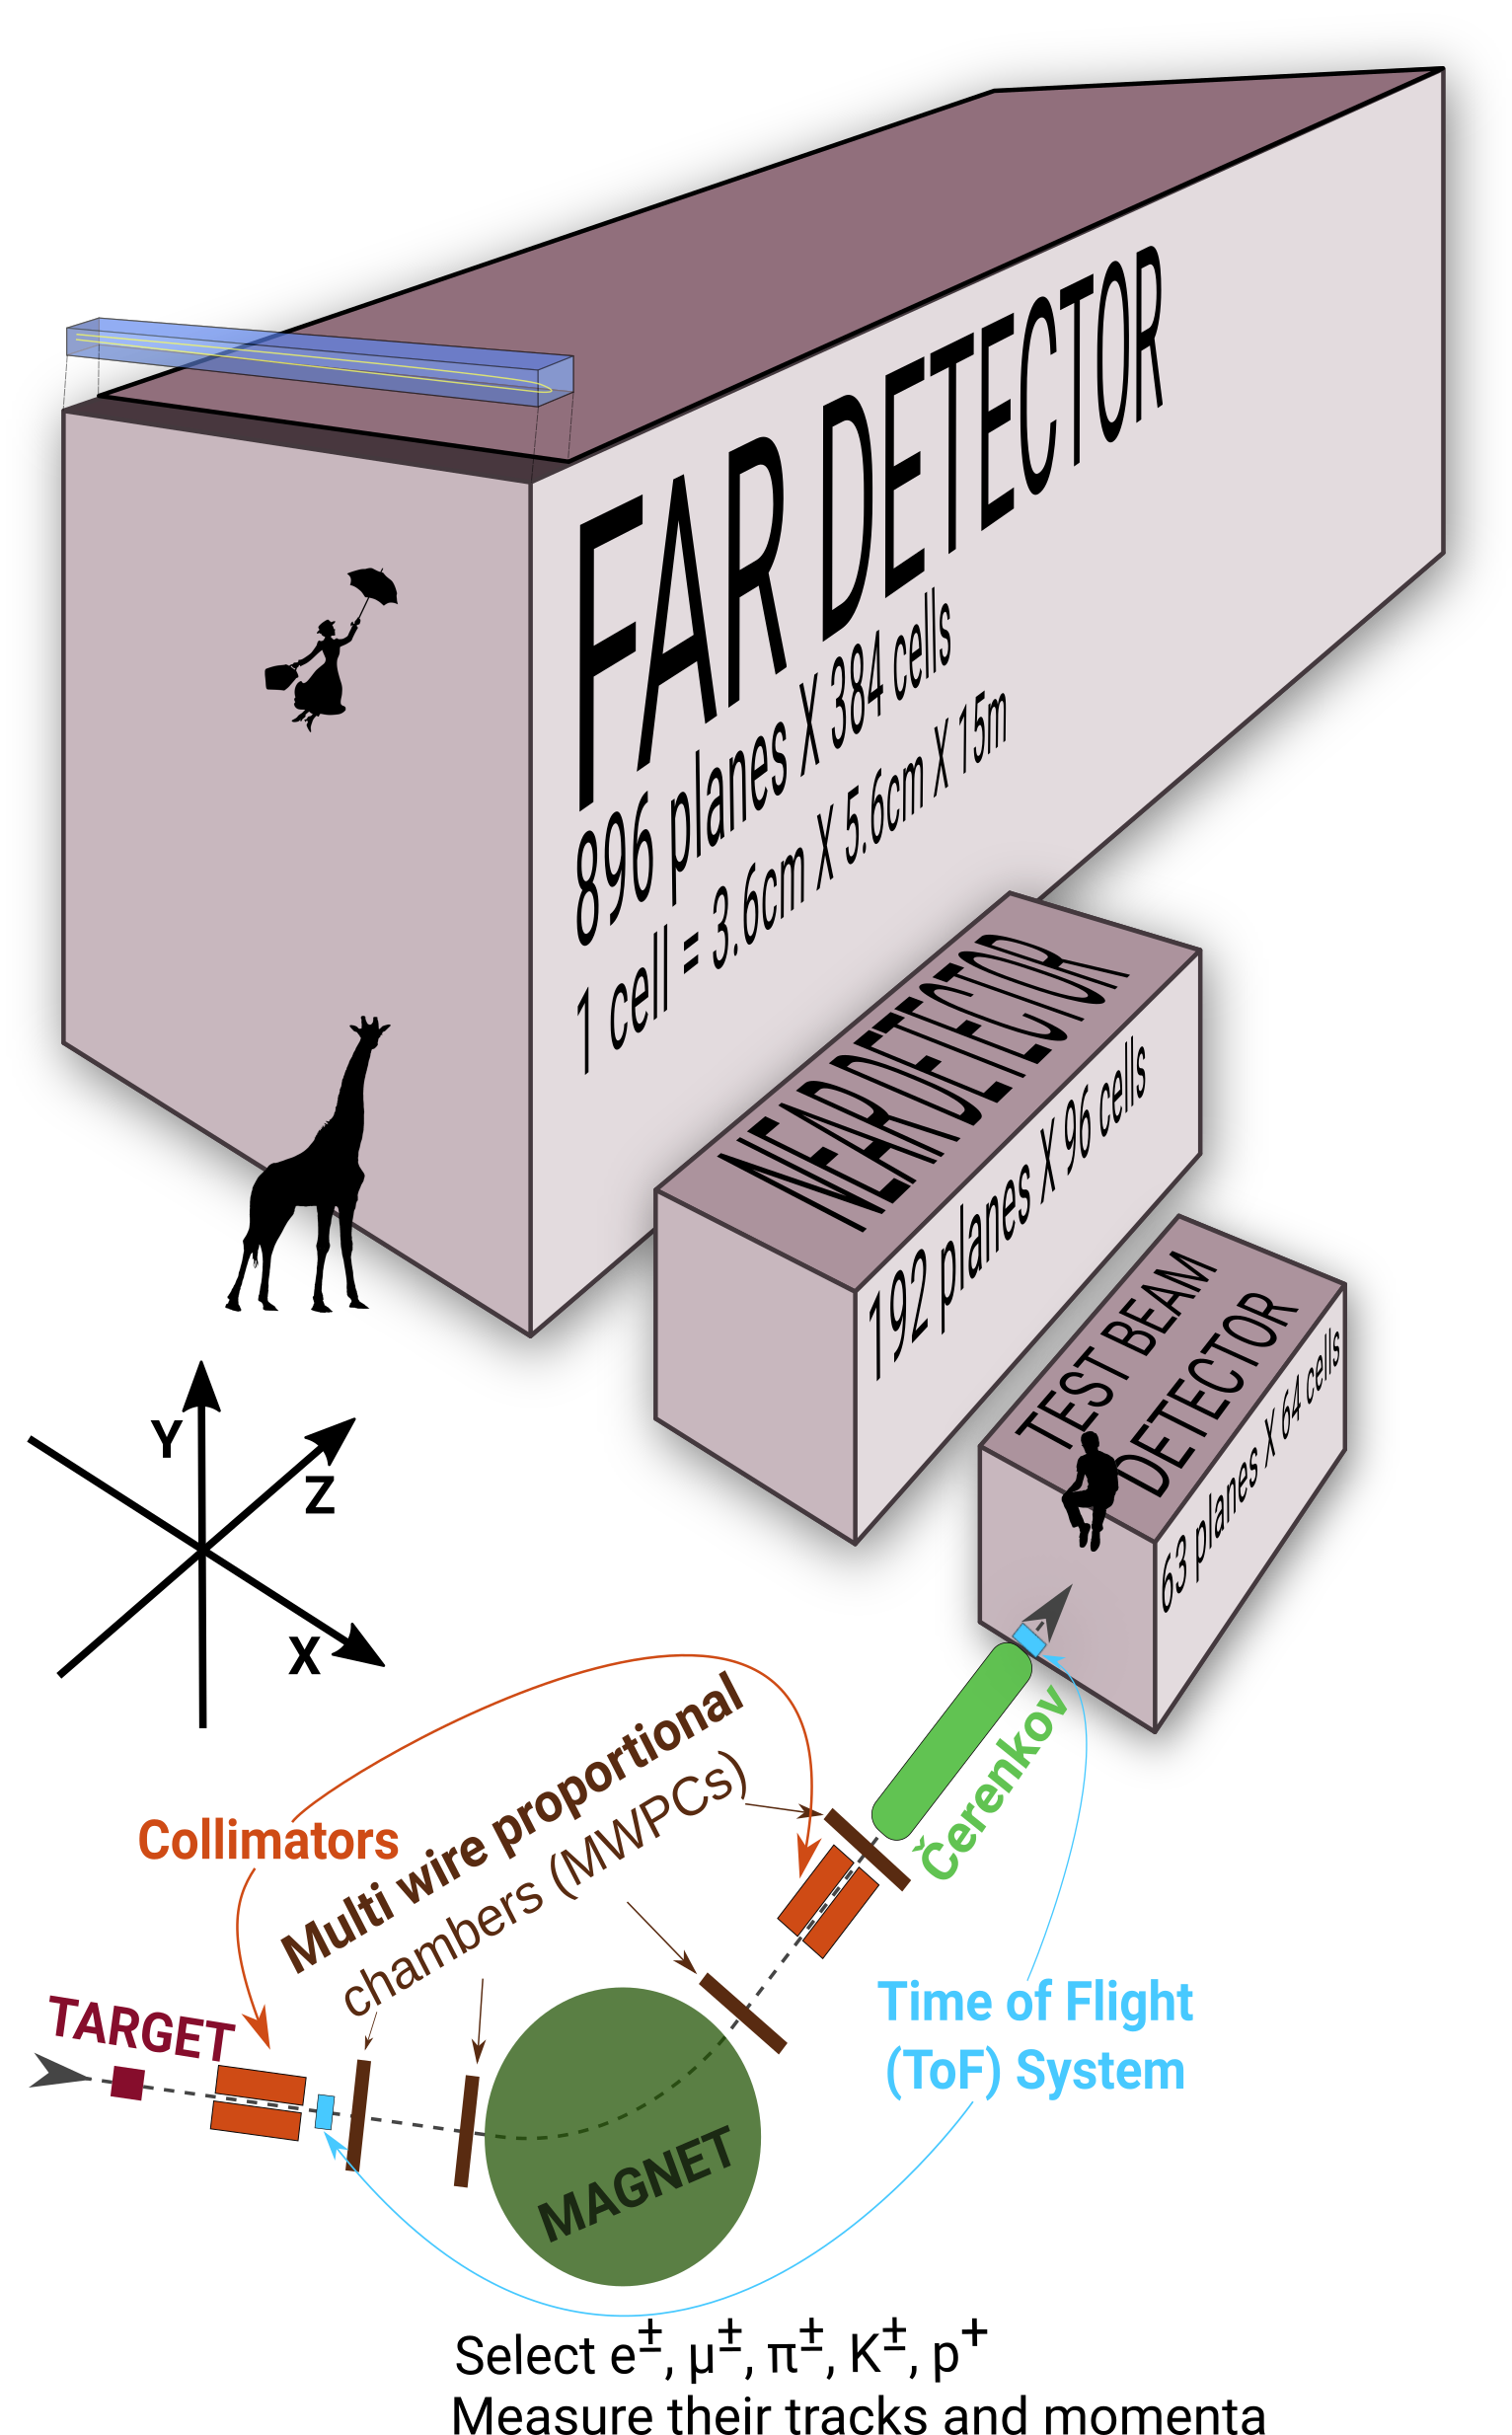
\includegraphics[width=.7\textwidth]{Plots/TBCalibration/TestBeamDetectorWithArrows.png}
\caption[Comparison of Test Beam detector to the Near and Far Detectors]{Comparison of Test Beam detector scale to the \acrshort{NOvA} \acrshort{ND} and \acrshort{FD} (and a man, giraffe, or Mary Poppins). Also shown are the Test Beam beamline detectors and components (not to scale), with arrows showing the direction of the beam. The three black arrows show the orientation of the detector coordinate system.}
\label{fig:TBDetector}
\end{figure}

%Should I aslo talk about the beam halo? Could that have an influence on the calibration? Maybe it's the peaks in the cosz distribution?

The Test Beam detector started with commissioning runs in June 2019 and ran, with an exception of regular summer shutdowns, until July 2022, after which it was decommissioned. The Test Beam data taking is divided into \textit{periods}, which are defined in Tab.~\ref{tab:TestBeamPeriods}. Period 1 only lasted for about a month and with only a half-filled detector, as explained below. It was therefore only used for detector commissioning and will not be used in any of the Test Beam physics analysis, or in the calibration.
\begin{table}[!ht]
\centering
\caption{Test Beam detector data taking periods.}
\def\arraystretch{1.4}
\begin{tabular}{l@{\hskip 1in}lcl}
Period 1 & June $3^{\textsf{rd}}$ 2019 & - & July $6^{\textsf{th}}$ 2019\\
Period 2 & December $5^{\textsf{th}}$ 2019 & - & March $20^{\textsf{th}}$ 2020\\
Period 3 & January $12^{\textsf{th}}$ 2021 & - & June $27^{\textsf{th}}$ 2021\\
Period 4 & November $30^{\textsf{th}}$ 2021 & - & July $10^{\textsf{th}}$ 2022
\end{tabular}
\label{tab:TestBeamPeriods}
\end{table}

Majority of the Test Beam detector and its instrumentation is identical to the other \gls{NOvA} detectors, with a few exceptions that could have an impact on the calibration. We are going to identify and discuss these differences in this section.

%[docdb:15750 - NOvA Test Beam task force report]: The test beam program was included in the NOvA proposal [1] and was considered as an essential part of the experiment since its inception. The main tangible result of these initial plans and later discussions was a production of special small extrusion modules, made at the end of the modules production stage, as possible components of a future test beam detector. In fact, this production followed and was based on initial simulations of a possible test beam experiment [5].

\subsubsection*{Beamline}
The beam for the Test Beam experiment originates from the same $\unit[120]{GeV}$ Main Injector protons used in \gls{NuMI}, extracted once a minute in a continuous $\unit[4.2]{s}$ spill~\cite{NOvATestBeamWallbangProceedings2020.pdf}. The protons are impinged on a copper target producing mostly protons and pions, which are then directed towards a second target, producing the tertiary beam of particles used in the Test Beam detector. As can be seen in Fig.~\ref{fig:TBDetector}, we use two collimators to direct the tertiary beam and a magnet to select the desired momentum. Particle tracking is done using the four \glspl{MWPC} and particle identification is done with a combination of \gls{ToF} detectors and a Cherenkov detector, set for electron detection.

\subsubsection*{Detector Parameters}
The \gls{NOvA} Test Beam detector consists of two 31-plane blocks, each beginning and ending with a vertical plane, with an additional horizontal plane glued in-between them to preserve the alternating pattern \cite{NOvA-doc-29543}. Each plane consists of 2 modules side-by-side, both made up of 32 cells. Each cell is $2.6\,\unit{m}$ long with an inner (without the PVC) depth and width of $5.9\,\unit{cm}$ and $3.8\,\unit{cm}$ respectively, same as for the other \gls{NOvA} detectors. This brings the final dimensions of the Test Beam detector to 63 planes $\times$ 64 cells, or $2.6\times 2.6\times 4.1\,\unit{m^3}$.

The 63 planes are numbered from 0 to 62, with even numbers corresponding to vertical planes and odd numbers to horizontal planes. Cells are numbered 0 to 63, going from bottom to top for horizontal planes and left to right, when facing the front of the detector, for vertical planes.

The detector coordinate system is illustrated in Fig.~\ref{fig:TBDetector}. It is centred with $\left(0,0,0\right)$ in the centre of the first plane \cite{NOvA-doc-58388}. The x axis runs left to right when facing the front of the detector, y axis from bottom to top, and z axis goes along the beam direction from front to the back of the detector. Position within each cell ($w$) is aligned with the x (y) axis for the horizontal (vertical) cells, with $w=0$ centred in the middle of each cell. The exact geometry of the Test Beam detector was measured in several alignment surveys and is saved in gdml files \cite{NOvA-doc-57955}.

In the past we encountered an issue when trying to align the Test Beam detector with the beamline measurements by rotating the detector. This broke several assumptions within the Test Beam geometry \cite{NOvA-doc-58388} and manifested as uncalibrated cells in the back of the detector \cite{NOvA-doc-57516}. This was fixed by realigning both the detector and the beamline separately, based on the last alignment survey, measured during the decommissioning of the detector.

%FD: maxPlane=900, maxCell=390. ND: maxPlane=220, maxCell=100. TB: maxPlane=63, maxCell=64

\subsubsection*{Scintillator}
%[TB task force report]: The NDOS decommissioning yielded 25000 gallons of scintillator. Since storage available is limited to 12000 gallons, it was decided to blend most of the 5000 gallons of existing ND/FD scintillator with the NDOS scintillator. 200 gallons of ND/FD scintillator, which has a slightly higher photon yield, are reserved for special studies. We also plan to reuse the NDOS secondary containment tub to provide oil+scintillator containment in case the test beam detector undergoes a catastrophic structural failure.

Test Beam used a combination of the leftover \gls{ND} and \gls
{FD} production scintillator oils and the oil drained from the \gls{NOvA} \gls{NDOS} test detector. The used scintillator oils also differ in the way they were stored since the \gls{ND} and \gls{FD} filling, or the \gls{NDOS} draining, which apparently impacted its quality. These factors have a significant effect on the energy deposition within them. The distribution of individual scintillator oils and the relative difference in their energy response can be seen in Fig.~\ref{fig:Scintillators}.

%The Test Beam detector is filled with several different versions of the NOvA scintillator oil, which differ mainly in the way they were stored since the filling of the near and far detectors. This is illustrated on figure \ref{figScintillators}.

\begin{figure}[!ht]
\centering
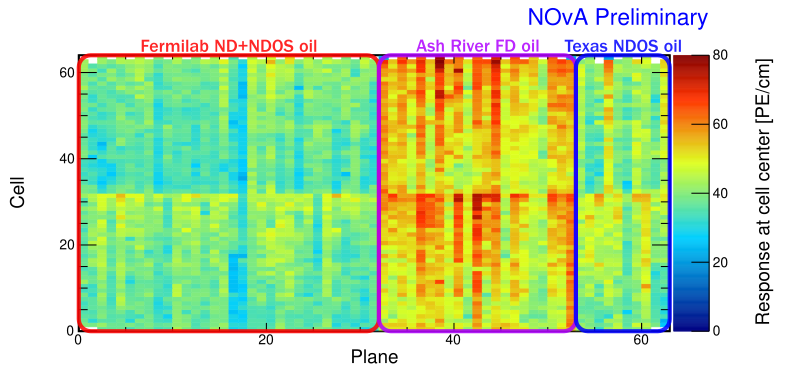
\includegraphics[width=\textwidth]{Plots/TBCalibration/TestBeamScintillatorOils.png}
\caption[Scintillator oils used in the Test Beam detector]{Uncorrected energy response in the centre of cells across the Test Beam detector showing a clear distinction between the different scintillator oils, labelled with coloured boxes and descriptions.}
\label{fig:Scintillators}
\end{figure}

We can distinguish four samples of \gls{NOvA} scintillator oil used in the Test Beam detector:
\begin{enumerate}
\item Mixed \gls{ND} production oil and \gls{NDOS}-drained oil stored in a tanker and four tanks outside in \gls{Fermilab} \cite{NOvA-doc-38349};
\item Separate \gls{ND} production oil and \gls{NDOS}-drained oil stored underground in barells at the MiniBooNE\footnote{MiniBooNE~\cite{MiniBooNEWebsite} is a \gls{Fermilab} experiment located close to the \gls{NOvA} \gls{ND}} cavern \cite{NOvA-doc-33012};
\item \gls{FD} production oil stored inside in Ash River in `totes' under several layers of black plastic \cite{NOvA-doc-34067};
\item \gls{NDOS}-drained oil stored mainly inside at Texas A\&M University and University of Texas at Austin \cite{NOvA-doc-38740, NOvA-doc-39088}.
\end{enumerate}

%The original plan \cite{NOVA-doc-34196} was to use the tanker and tank scinitillator for the entire Test Beam detector. However, due to extreme cloudeness of the scintillaotr in the tanks 

The original plan \cite{NOvA-doc-34196} was to only use the tanker/tank scintillator (sample \#1). First tests showed acceptable results and the tanker oil was used to fill out almost the entirety of the first block of the detector (first 32 planes) \cite{NOvA-doc-38349}. However, when we loaded oil from tank \#2 into the tanker, it became extremely cloudy and unusable, possibly due to contamination with water accumulated at the bottom of the tanks. The rest of the first block was therefore topped up with high quality scintillator from \gls{NDOS} (sample \#2). This is labelled as `\gls{Fermilab} \gls{ND}+\gls{NDOS} oil' in Fig.~\ref{fig:Scintillators}.

%NDOS+ND scin3llator were stored in MEast tank farm in translucent tanks open to the atmosphere in 2016 [docdb:41229]
%docdb:41229 actually contains a pretty good description of the whole story

%First Tanker (2730 gallons pumped) used to fill 97.5% of first block ... Missing ~2.5 gallon top-off... Decided to use reserved NDOS 55-gallon drums... Used 65 gallons for detector, 11 gallons to clean up fill lines

%Even before the extreme cloudiness was discovered, it was known that the oil from the tanks has lost much of its original light yield properties. Reasons vary from water contamination to insects and dirt contamination \cite{NOVA-doc-34046-v2}. Yet it was still decided to use the tank 2 oil \cite{NOVA-doc-34196}. It was also decided not to mix the various oils (tanker/tank/NDOS/Ash River) as studying energy deposition in different types of oils could lead to some interesting insights \cite{NOVA-doc-34046-v2}.

%"One of the promising studies we see coming out of this is to understand the differences in performance for different type of energy depositions of scintillator A vs B vs C. " [docdb:34046]

The first 21 planes of the second block (planes 32 to 52) were filled with the \gls{FD} production scintillator shipped in from Ash River (sample \#3) \cite{NOvA-doc-41961}. We again topped up these planes with the \gls{ND}+\gls{NDOS} scintillator (sample \#2).

The last 10 planes (planes 53 to 62) \cite{NOvA-doc-41961} were filled with the `Texas' scintillator (sample \#4), which has higher light yield than the one from the tanker, but lower than the Ash River one \cite{NOvA-doc-38740}.

%[docdb:38349] 2730 gallons of scintillator transferred to detector from the tanker. On April 16, circulated 20 gallons from tanker, and took scintillator sample. Extreme cloudiness meant 0\% light transmission (>=95\% required). Strongly suspect problem due to water accumulated at the bofom of tankers vented to the atmosphere since 2016, mixed with oil by pump. Used 2/4 reserved NDOS 55-gallon drums for top-off...  completed top-off of all Block 0 modules

In total the Test Beam detector is filled with 5418 gallons of scintillator oil with a weight of approximately 28.6 tons \cite{NOvA-doc-29543}.

\subsubsection*{Readout}
The Test Beam detector uses in total 126 \glspl{FEB}, each reading out signal from 32 cells \cite{NOvA-doc-29543}. The readout is located on the top and right side (when looking at the front) of the detector. 118 \glspl{FEB} are version 4.1, same as in the \gls{FD}, and 8 \glspl{FEB}, located in pairs on planes 16, 17, 48 and 49, are version 5.2, same as in the \gls{ND}. As was described in Sec.~\ref{sec:DAQ}, the \gls{ND} \glspl{FEB} are designed to read out data at a faster rate and using a mix of \gls{FEB} types allows us to study the difference in their response and to validate both versions in the same environment~\cite{LackeyThesisNOvATBProtons2022.pdf}.

%The Near and Far Detectors use different front-end electronics since they handle different data volumes; the Test Beam Detector is instrumented with both types to facilitate a complete characterization of both NOvA neutrino detectors. [NOvATestBeam.pdf - Mike's proceedings]

\subsubsection*{Environment}
Unlike the \gls{ND} and the \gls{FD}, the Test Beam detector does not have any overburden to shield it from cosmic particles, which affects their rate and energies inside the detector. There is also less precise control of temperature and humidity than in the other detectors [source?], which can potentially impact the scintillator and readout performance.
\todo{Finish this description of environmental control, maybe mention HVAC? - depends how much I want to talk about this effect...}

%Is the HVAC the only systema that is controling the environment at MC7b?

%From docdb:29543
%Temperature very stable during winter months (heaCng is installed at MC7). However, dew point went over 10C ND shutdown threshold several times.
%Alex'es summary in docdb:30750:
%Ordered HVAC unit with electric reheat and dewpoint control, in essence over-cooling to maintain dewpoint then reheat to maintain temperature.

%Can I describe what is the shielding in MC7b? What is the white stuff from? It's basically the only thing shielding the detector from the cosmics and temperatures. Also need to say there is an HVAC system

%Placed in the Fermilab Test Beam Facility with no overburden. Describe environmental controls, temperature dependence etc. Maybe add plots from environmental control (temperature differences etc.) with descriptions of where were the readings taken.

\subsubsection*{Underfilled Cells Issue}
The Test Beam detector is slightly tilted around the z axis by about $0.7^{\circ}$ towards the readout. This caused the top cells of both modules of all the horizontal planes (cells 31 and 63) to be underfilled, creating an air bubble on the left side of the detector and severely affecting the energy response in those cells \cite{LackeyThesisNOvATBProtons2022.pdf}. This was fixed \cite{NOvA-doc-49439} during the period 3 running by adding extensions to the filling ports and overfilling the horizontal cells with the \gls{ND}+\gls{NDOS} scintillator (sample \#2 from the scintillator description). More details on this issue and its effects and on how it was handled in calibration are detailed in Sec.~\ref{sec:TBCalibration_period3}.
%This scintillator was also used in the first half of the detector (Fermilab ND+NDOS oil on figure \ref{figScintillators}), but is different from the "Ash River oil" used in part of the second half of the detector (bright part of figure \ref{figScintillators}). The overfilling was done in April 2021 in 3 stages in between the full operation of the Test Beam detector.

%The detector is tilted around z axis towards the readout by about 0.7 degrees (the largest tilt is for the 11th plane of 0.79330 degrees. The ND has an oposite tilt of -0.2515 degrees on average (but also the readout is on the opposite side, so is it actually the same tilt?). Correcting this by 8 degrees would require lifting the east edge by at least 3.66cm, or to correct it to the ND tilt by lifting the east edge by 4.17cm. [docdb:47491 - this is the original talk by Teresa explaining the tilt on 21st Sep 2020]

%Also need to mention that the detector was then overfilled [docdb:49439 or 49827] but with a scintillator from the NDOS drums, causing the discrepancy between the high quality Ash River scintillator and the NDOS scintillator. But need to mention this after the scintillator part.
%The overfilling was done in three stages:
%\begin{enumerate}
%\item Overfilling the back 9 horizontal and the 7th horizontal from the front by April 21st
%\item Overfilling of the 15 front cells (except the 7th, which was already done, and the 14th, %with problems drilling vent hole) by April 27th
%\item Overfilling of the remaining 8 horizontals by April 30th
%\end{enumerate}

%From Teresa's thesis:
%The pitch and yaw of the detector was 2.464◦ around x and 0.487◦ around z. Roll (around beam direction) of each plane. Unfortunately, the direction of the roll means the east side of the detector is slightly lower than the west side. The east side is where the readout and fill ports for the scintillator are. As a result, the top cell in each horizontal module is underfilled, with an air bubble on the west side.

%%%%%%%%%%%%%%%%%%%%%%%%%%%%%%%%%%%%%%%%%%%%%%%%%%%%%%%%%%%%%%%%%%%%%%%%%%%%%%%
%%%%%%%%%%%%%%%%%%%%%%%%%%%%%%%%%%%%%%%%%%%%%%%%%%%%%%%%%%%%%%%%%%%%%%%%%%%%%%%
%%%
%%%                      Data based simulation of cosmic
%%%
%%%%%%%%%%%%%%%%%%%%%%%%%%%%%%%%%%%%%%%%%%%%%%%%%%%%%%%%%%%%%%%%%%%%%%%%%%%%%%%
\section{Data-based Simulation of Cosmic Muons}\label{sec:DataBasedSimulation}
The standard \gls{NOvA} calibration procedure described in Sec.~\ref{sec:NOvACalibration} uses the \gls{CRY} \gls{MC} generator (see Sec.~\ref{sec:NOvASimulation}) to create the simulated cosmic ray sample for calibration. However, the \gls{CRY} simulation proved to be highly inefficient, with only a small fraction of the simulated cosmic-ray activity resulting in selected calibration hits and the majority of particles failing to even hit the detector. This inefficiency consumed significant processing resources, disk space, and file usage. Moreover, the momentum and angle distributions in \gls{CRY} were not well suited to the \gls{NOvA} sites, potentially impacting the calibration accuracy.

To overcome these challenges, we developed and implemented a data-based simulation that eliminates the need for the \gls{CRY} \gls{MC} generator. Instead, we use a subset of the cosmic data sample used in calibration and pass it through the beam removal filter, reconstruction chain and a selection of high-quality cosmic muons. The selected cosmic muon events are then used as inputs to the detector simulation to create a new simulated cosmic ray sample.

This approach results in a near-perfect efficiency, ensuring that almost every simulated muon contributes to the final calibration sample, thus saving processing time, file size, and storage. Additionally, the simulated muon distributions are inherently consistent with the distributions from data. Given that the calibration chain itself is a time and computing intensive process, the reduction in simulation files and their sizes has significant benefits downstream of the file generation. 
%On the other hand, using real data to seed the simulation could introduce undesirable bias, if we do not carefully consider possible misreconstruction or selection bias.\note{Can I re-word the last sentence?}
%Using real world data introduces bias from known and unknown effects, such as varying detector efficiency or readout faults... We need to carefully consider and mitigate these effects when creating the simulation to make sure of its validity

\subsection{Reconstruction and Selection of Cosmic Data Events}\label{sec:CosmicGenAna}
It is important to choose a data sample that represents the detector in an ideal state, with as few known issues as possible. For Test Beam, we chose the period 4 data sample (see Tab.~\ref{tab:TestBeamPeriods}), as the other periods had complications such as faulty \gls{FEB}s, or underfilled cells. We only used half of the entire period 4 sample by only using every other sub-run for the simulation to only produce the necessary number of events for a successful calibration.

%Our goal is to examine the response of the \textbf{simulated detector} to realistic cosmic muons found in the \textbf{real data}. We therefore need to use well-reconstructed and selected cosmic muons from data to generate our simulation. If the selection of the reconstructed data does not accurately correspond to reality, either due to misreconstruction or incorrect selection criteria, it can introduce bias into our simulation.

We designed the reconstruction and selection criteria so that the majority of the simulated cosmic muons make it into the final simulation calibration sample. Therefore, we employed a similar process to that used to create the data calibration samples. Additionally, we require all distributions of the selected events to be well-understood and to resemble those of the data calibration samples.

\subsubsection*{Remove Beam Spills}
The first step is to remove beam spill events based on their time relative to the time of the beam spill. For Test Beam the beam spill is $\unit[4.2]{s}$ long and we remove all events within a $\unit[5]{s}$ window from the start of the beam spill, as shown in Fig.~\ref{fig:RemoveTBSpills}. This should leave us with mostly cosmic events.

\begin{figure}[hbtp]
\centering
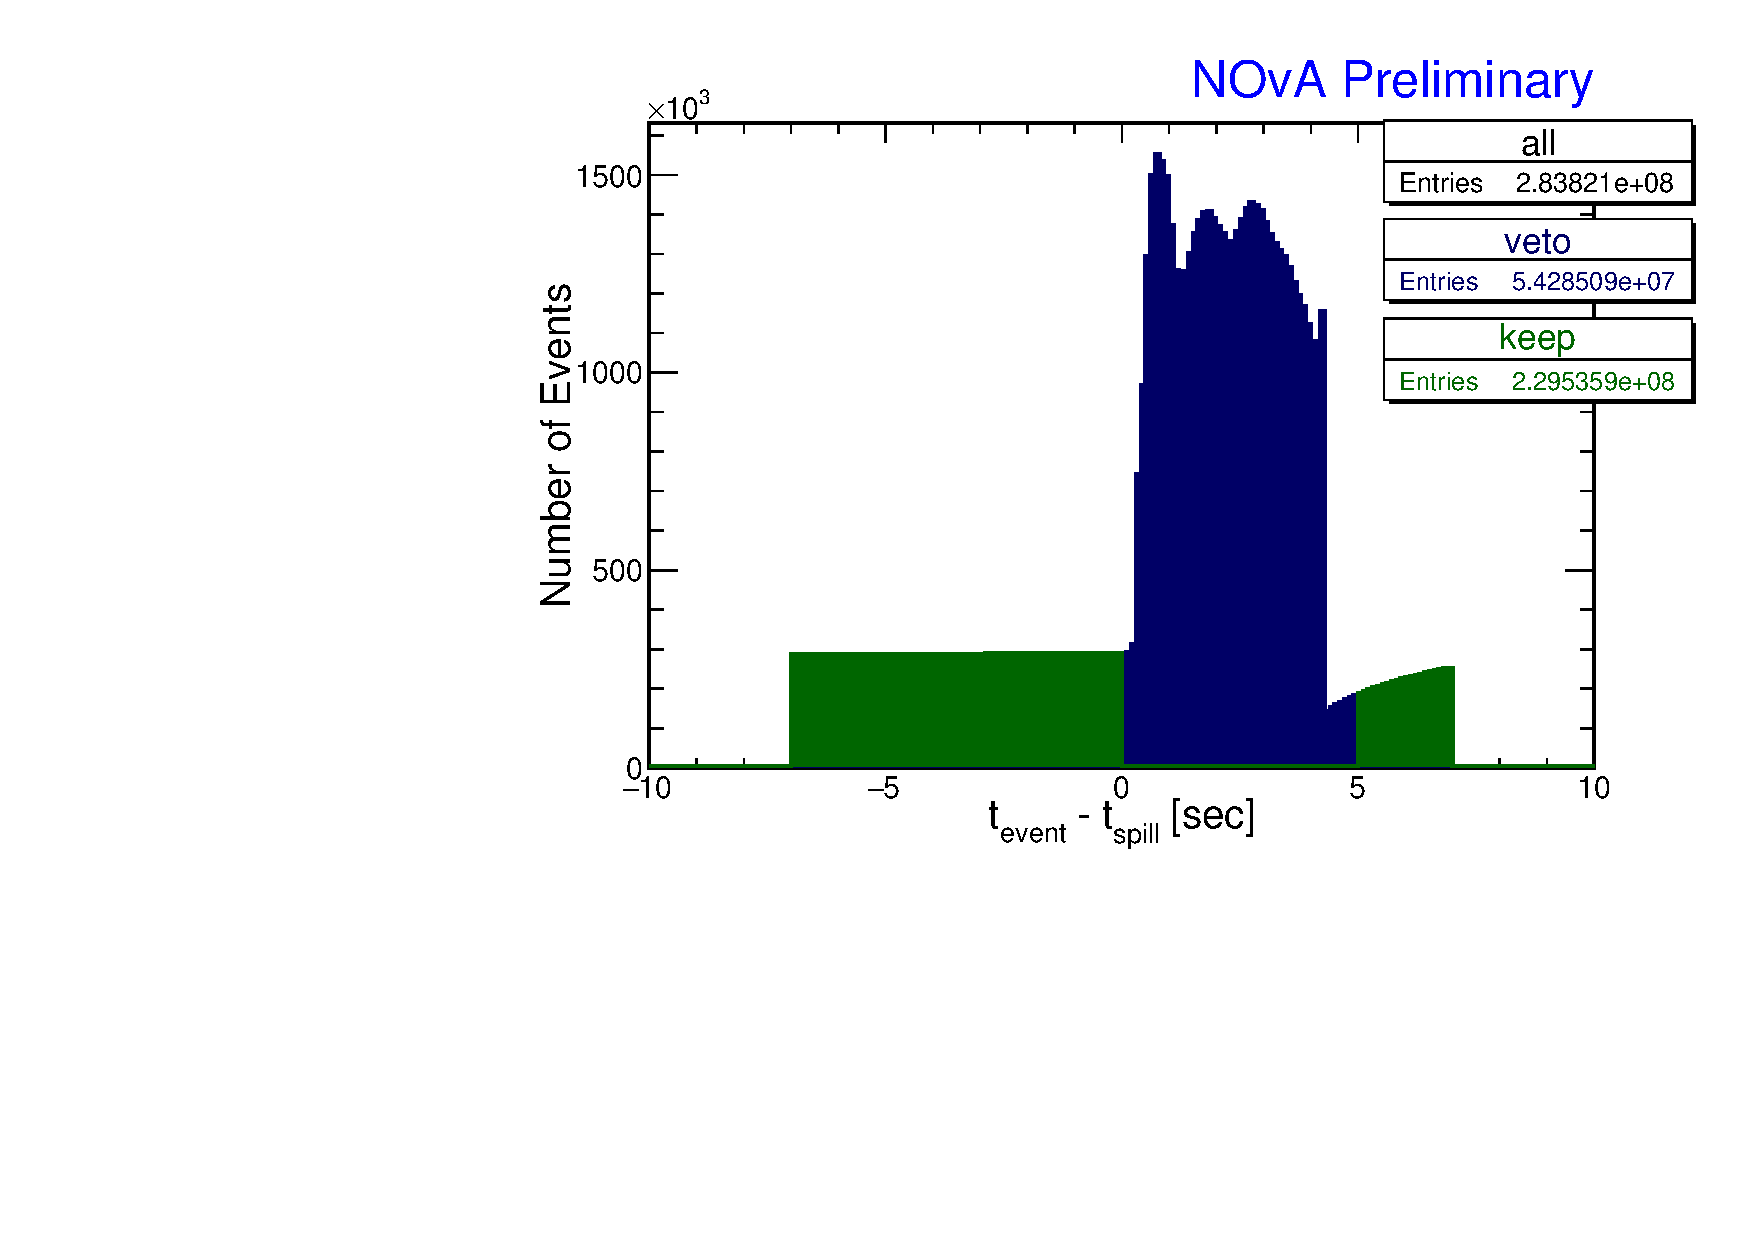
\includegraphics[width=\textwidth]{Plots/TBCalibration/RemoveTBSpills.pdf}
\caption[Removing Test Beam beam spill]{Test Beam beam spill events removed (blue) from the calibration samples. The remaining events (green) should mostly consist of cosmic particles. This example and the numbers of entries are for the full period 4 Test Beam sample.}
\label{fig:RemoveTBSpills}
\end{figure}

\subsubsection*{Reconstruction}
To use the events in the simulation, we require their vertex positions and their initial 4-momenta. We use the standard reconstruction methods from \gls{NOvA}, described in Sec.~\ref{sec:NOvAReconstruction}. First we take the raw hits and group them into slices. Then we reconstruct cosmic tracks using the window cosmic track algorithm (used for calibration samples). Since we also require the 4-momentum information we have to use the \gls{BPF} tracking algorithm to identify muons and assign their momenta. \gls{BPF} required a vertex and prong input information, which we get from a cosmic ray vertex and FuzzyK prong algorithms respectively. The first three steps are identical to the full reconstruction applied to get the calibration samples. Since we do not need a 4-momentum information for calibration, we do not need to use cosmic ray vertex, FuzzyK vertex, or the \gls{BPF} to create calibration samples.

\subsubsection*{Selection}\label{sec:DataBasedSimSelection}
After the reconstruction process, we proceed to select events based on their slice' and \gls{BPF} track's properties. The overview of all selection criteria and their corresponding cut values are listed on Tab.~\ref{tab:DataBasedSimEventSelection}. In detail, the following conditions are used to select cosmic muon events for the data-based simulation:
\begin{enumerate}
\item We only use successfully reconstructed 3D \gls{BPF} tracks with the muon assumption;
\item As we aim to select cosmic events originating outside the detector, we apply a cut based on the distance of each track's start position from the edges of the detector. This cut has a negligible impact on the \gls{BPF} tracks, as indicated by the minimal difference between the red and the dotted azure lines in Fig. \ref{fig:DataBasedSimCosZSelectionComparison};

\begin{figure}[!ht]
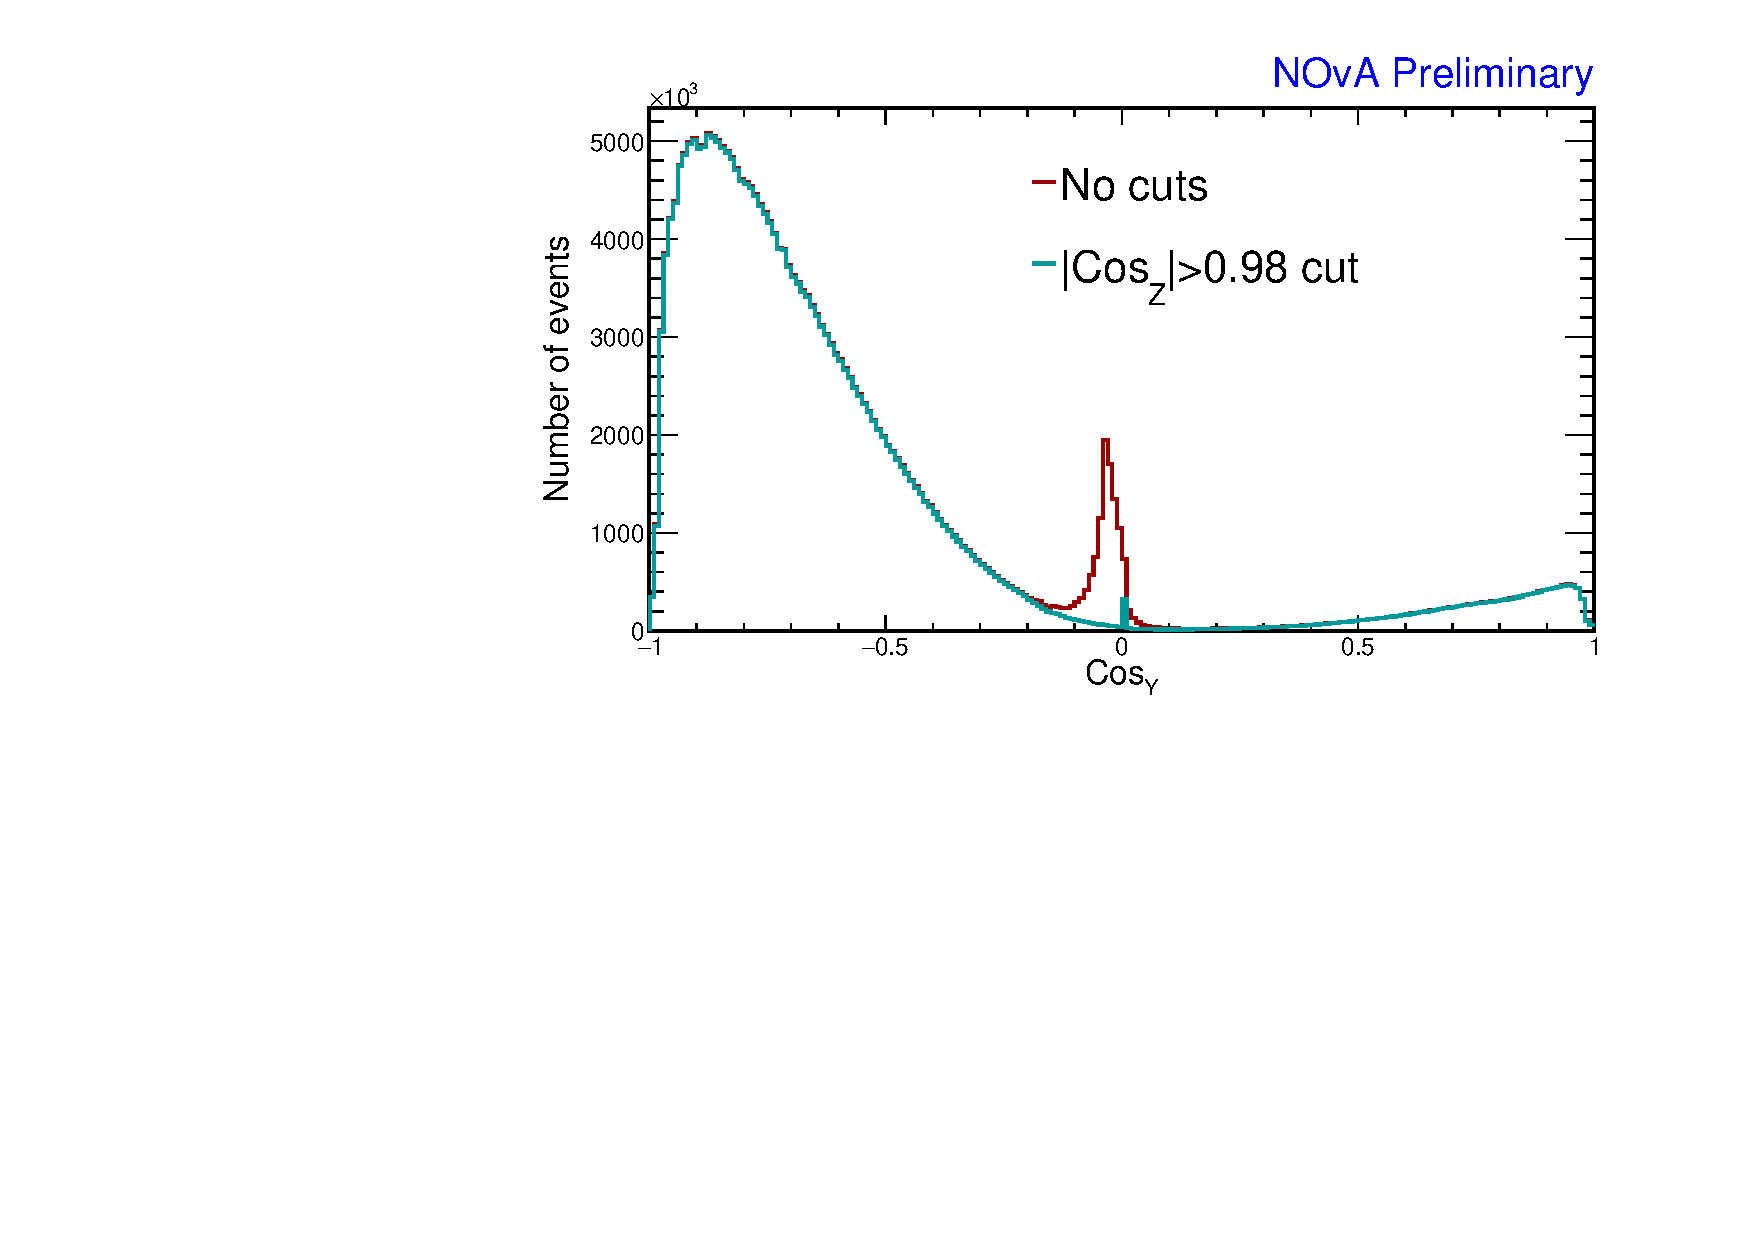
\includegraphics[width=\textwidth]{Plots/TBCalibration/DBSim_SelectionComparisonCosZCut_CosY.pdf}
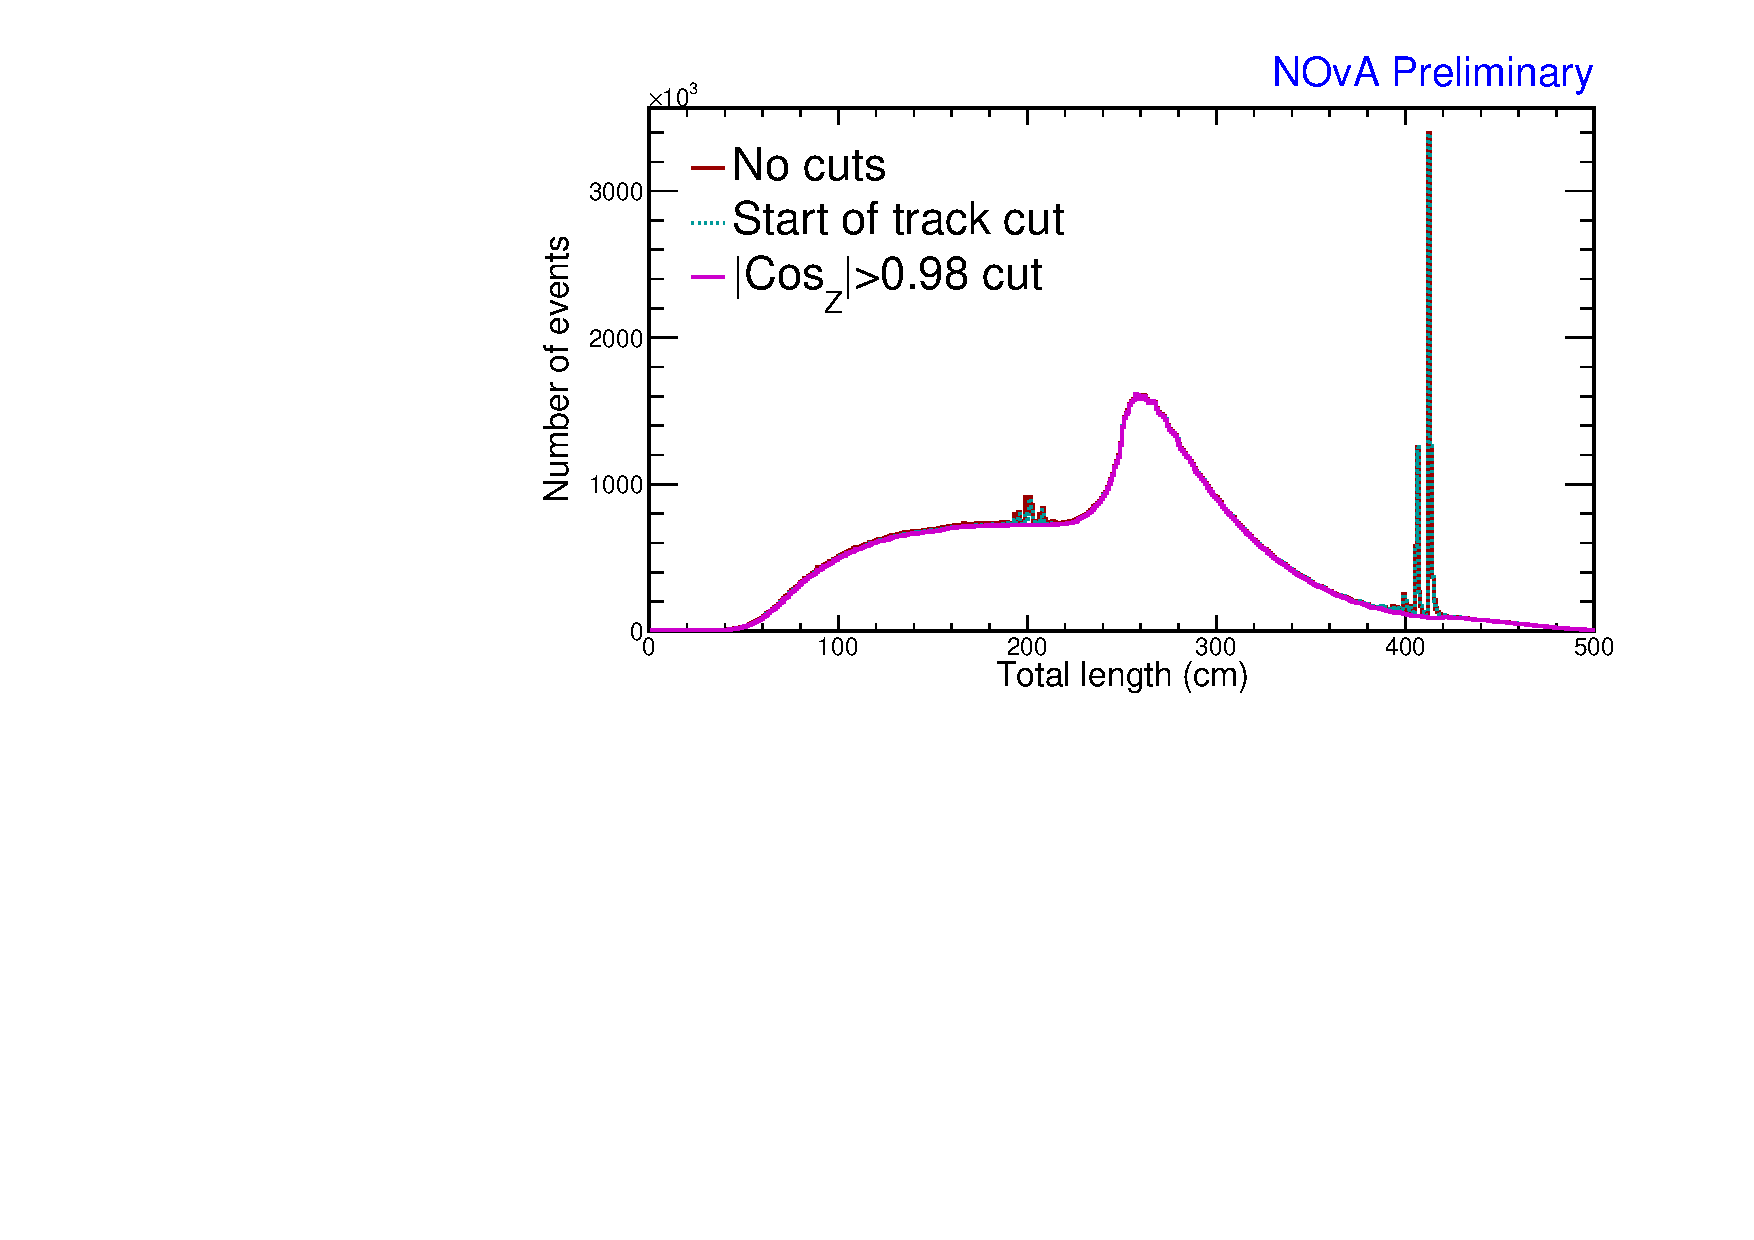
\includegraphics[width=\textwidth]{Plots/TBCalibration/DBSim_SelectionComparisonCosZCut_TotLength.pdf}
\caption[Track start and $\textsf{Cos}_Z$ cut for data-based simulation selection]{Impact of track start and maximum track angle from the z axis ($\textsf{Cos}_Z$) cuts on the Test Beam data for the data-based simulation of cosmic muons. The track start cut has only negligible effect. The maximum $\textsf{Cos}_Z$ cut effectively removes sharp peaks in the total track length distribution and events perpendicular to the Y axis. These events are all parallel with the Z axis and are most likely leftover beam events. All of the distributions are made from the period 4 Test Beam data.}
\label{fig:DataBasedSimCosZSelectionComparison}
\end{figure}

\item We remove all events whose track is parallel to the beam direction, by requiring the angle from the Z (beam) axis to be $|\textsf{Cos}_Z|\leq 0.98$. Figure \ref{fig:DataBasedSimCosZSelectionComparison} demonstrates the presence of events peaked at track lengths of approximately $\unit[410]{cm}$ and $\unit[200]{cm}$, which correspond to the total and half length of the detector, respectively (or alternatively lengths of both modules and a single module). These events are strictly parallel to the beam direction and are likely remnants of beam events. Applying a cut on $\textsf{Cos}_Z$ effectively removes these events without affecting the rest of the data. This cut might only be needed for the Test Beam detector and not for the near and far detectors.

\item To ensure that only events contributing to the final calibration sample are simulated, we use a selection based on the cuts used to select events for the data calibration samples (see Sec.~\ref{sec:NOvACalibration}). We call these cuts the \textbf{calibration cuts}. However, there are two caveats we need to consider when applying the calibration cuts:
\begin{enumerate}
\item First, to create calibration samples, we apply the selection on tracks from the \textbf{Window cosmic track} algorithm instead of the \gls{BPF} algorithm, which yield different distributions as depicted in Fig.~\ref{fig:DataBasedSimTrackComparison}. Notably, the \gls{BPF} tracks have a hard cut-off at the detector edges, whereas the Window cosmic tracks are allowed to start beyond these limits. Also, the \gls{BPF} tracks have a rugged distribution in $\textsf{Cos}_Z$, which is not present for Window cosmic tracks. This is likely caused by the detector structure, as shown in Fig.~\ref{fig:DataBasedSimBPFPeaks}, but it is not clear how. We concluded that he rugged shape does not have any impact on the resulting simulation. Given these differences between the tracking algorithms, applying the calibration cuts on \gls{BPF} tracks could mistakenly remove events that would pass the same selection when applied to the Window cosmic tracks.

\begin{figure}[!ht]
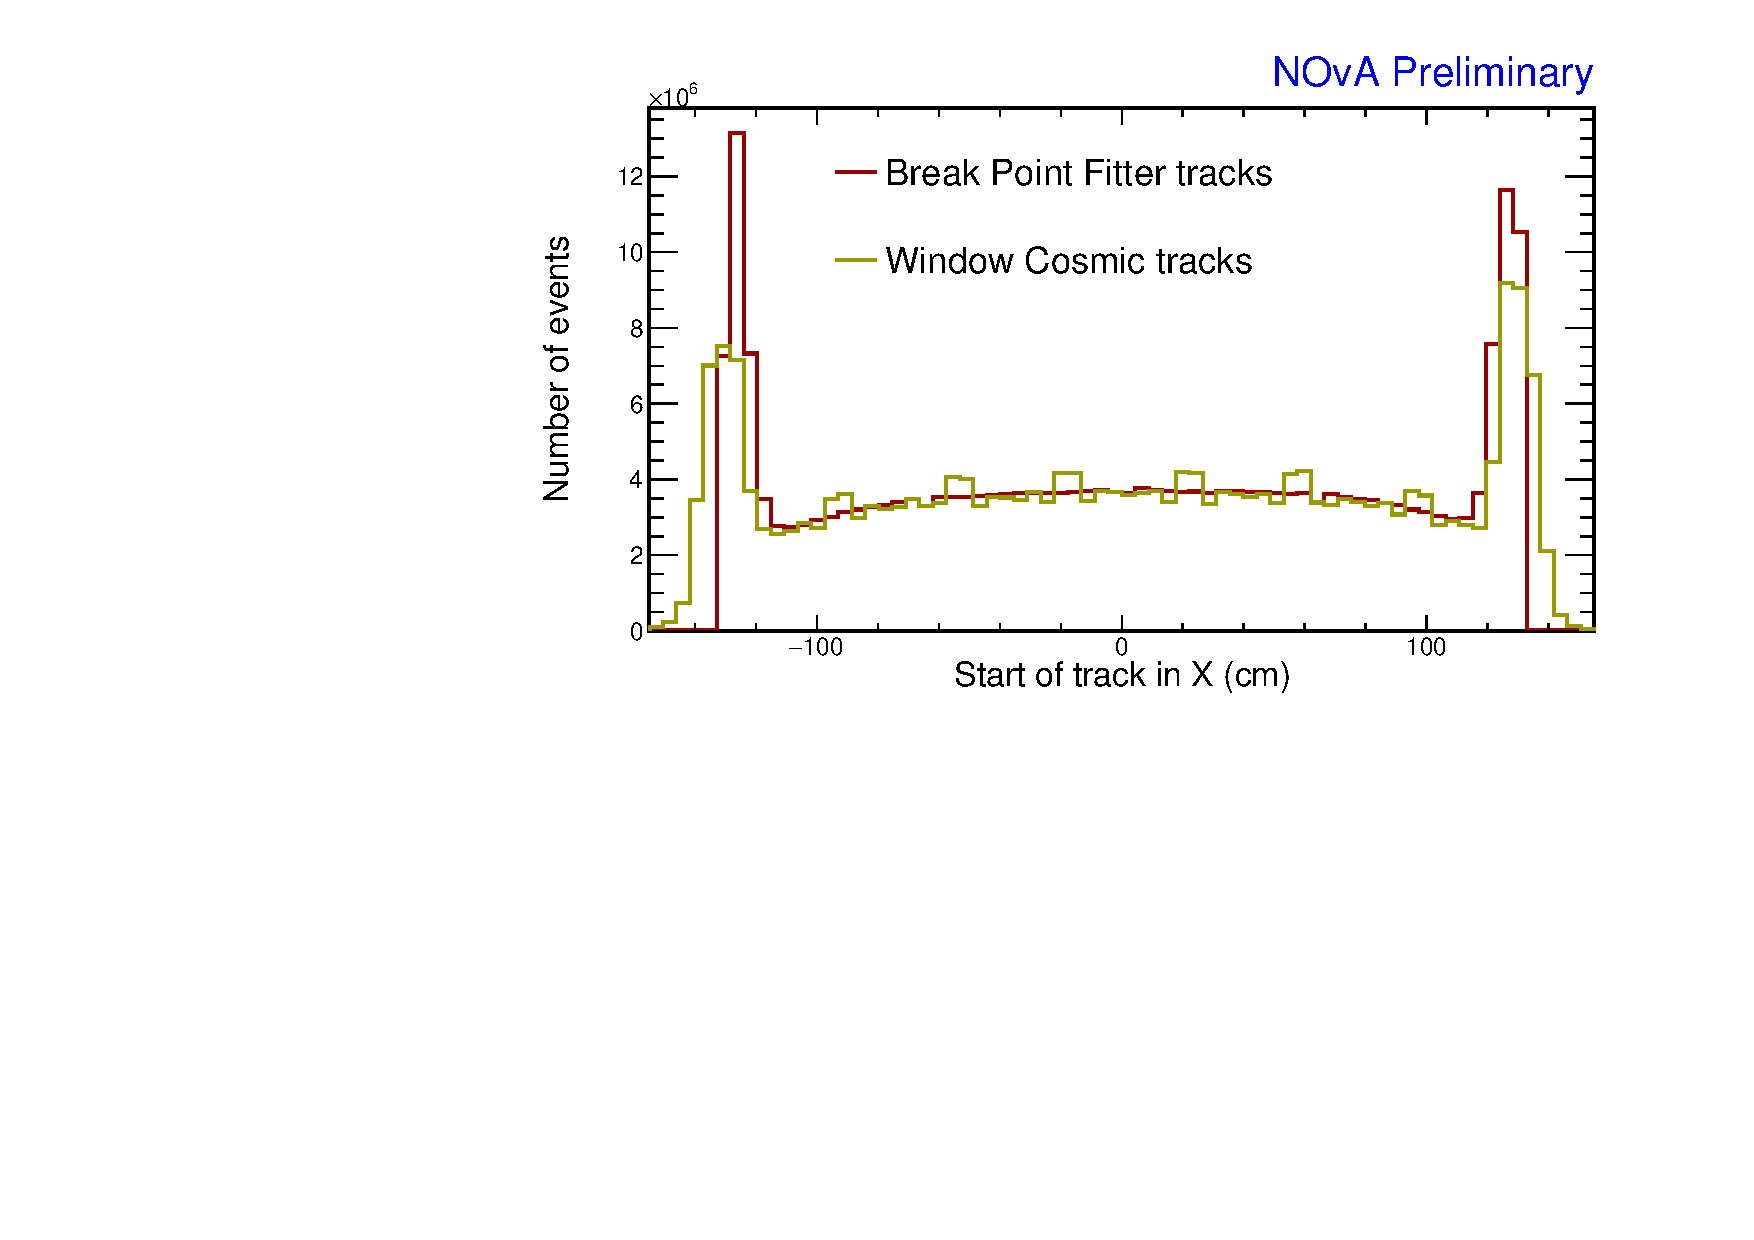
\includegraphics[width=\textwidth]{Plots/TBCalibration/DBSim_TrackAlgComparison_StartX.pdf}
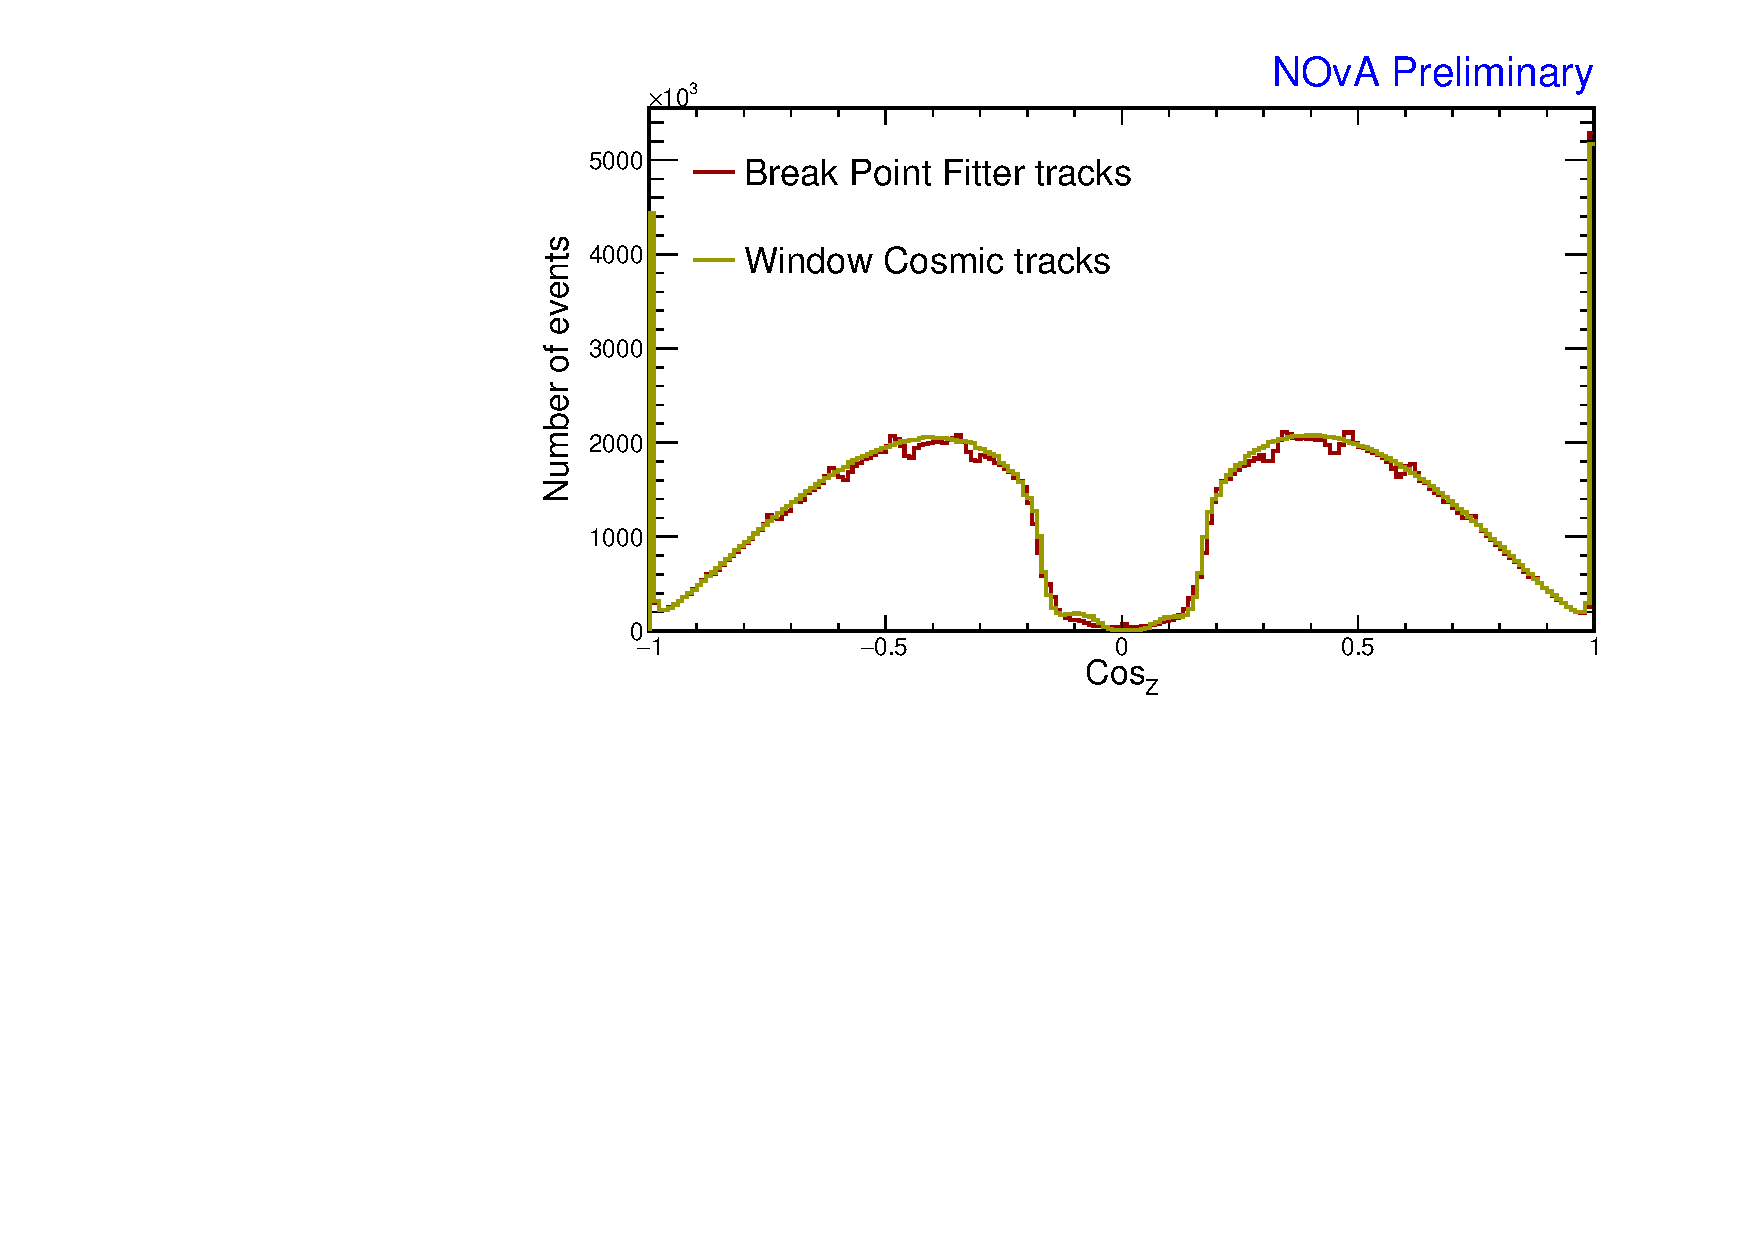
\includegraphics[width=\textwidth]{Plots/TBCalibration/DBSim_TrackAlgComparison_CosZ.pdf}
\caption[Tracking algorithms for the data-based simulation selection]{Difference between the tracks reconstructed with the \acrshort{BPF} and with the Window cosmic track algorithms. Both distributions are for the period 4 Test Beam data (with removed beam spill) without applying any selection.}
\label{fig:DataBasedSimTrackComparison}
\end{figure}

\begin{figure}[!ht]
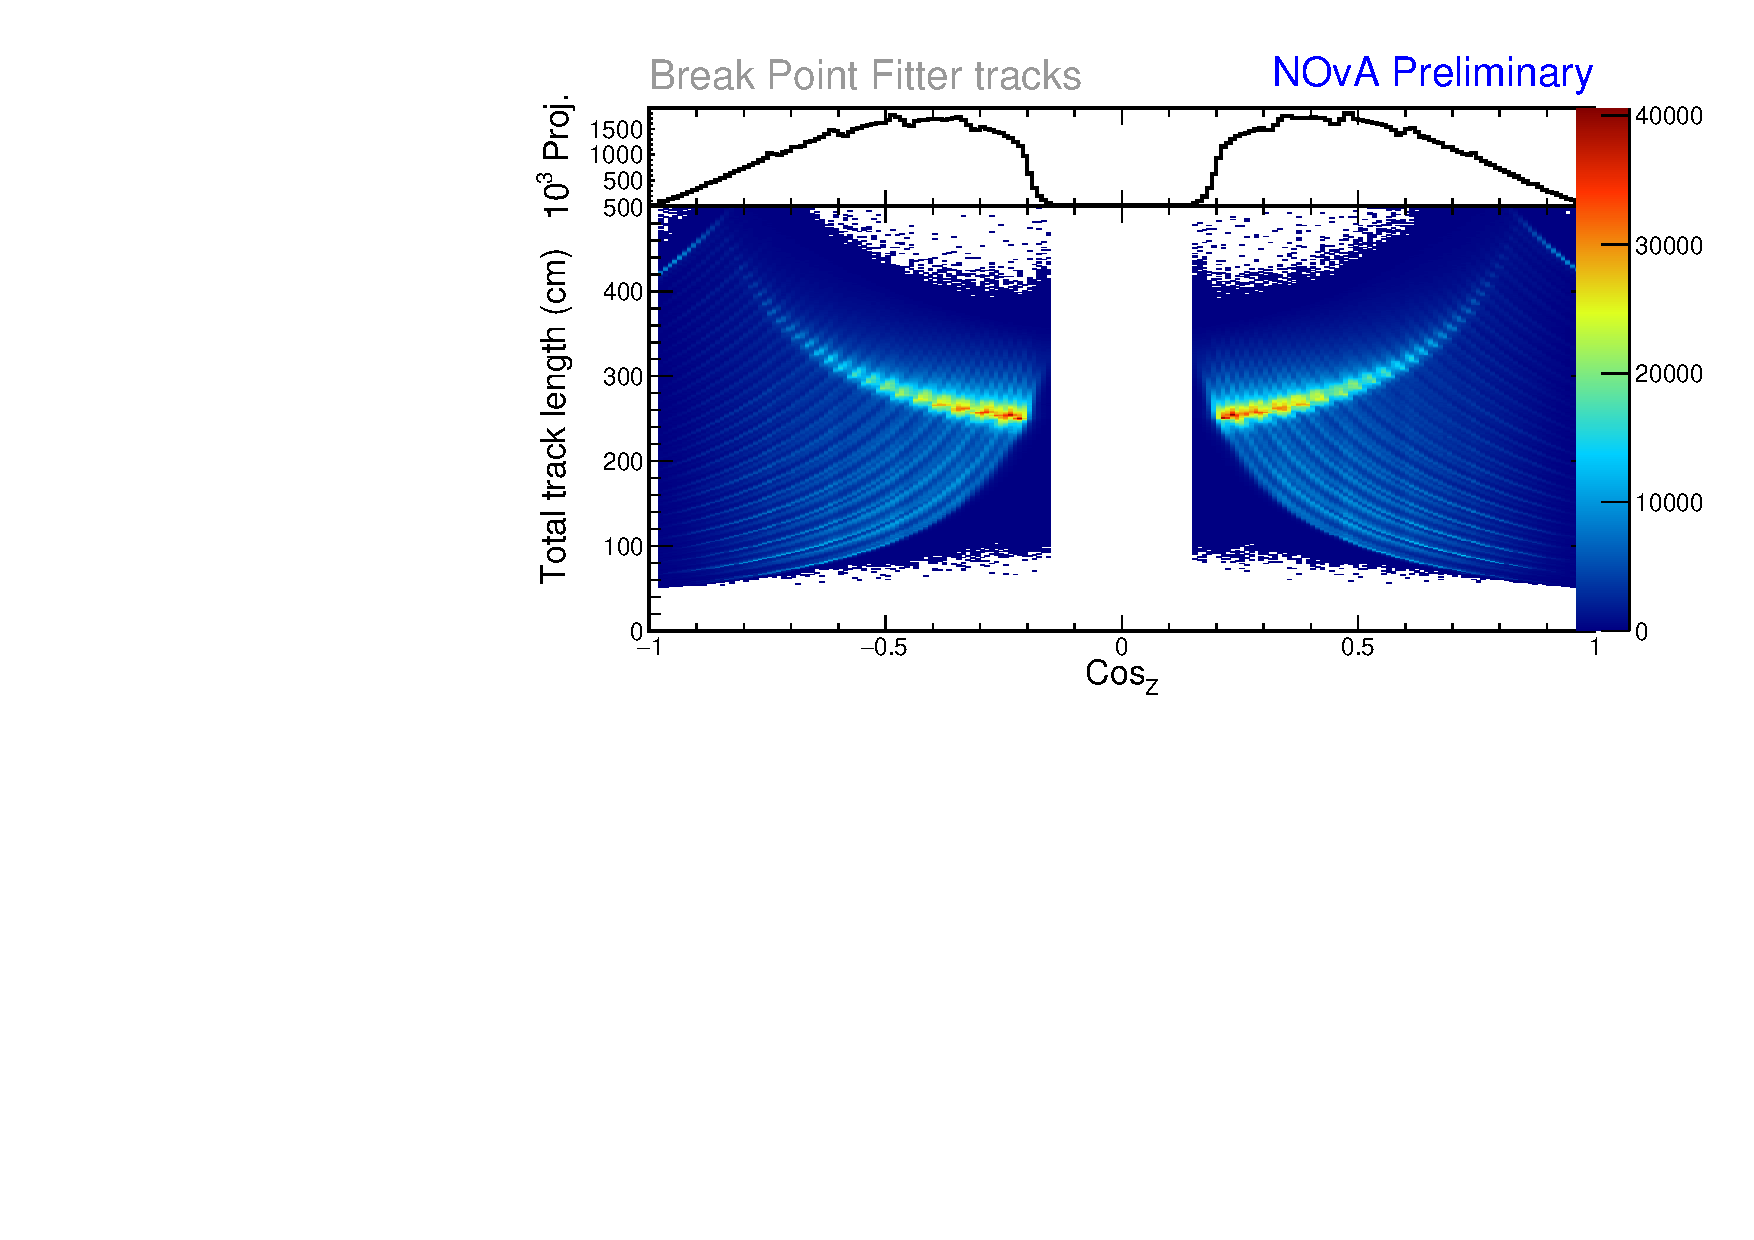
\includegraphics[width=\textwidth]{Plots/TBCalibration/DBSim_BPFPeaks_BPFTracks_dcosz_TotLength.pdf}
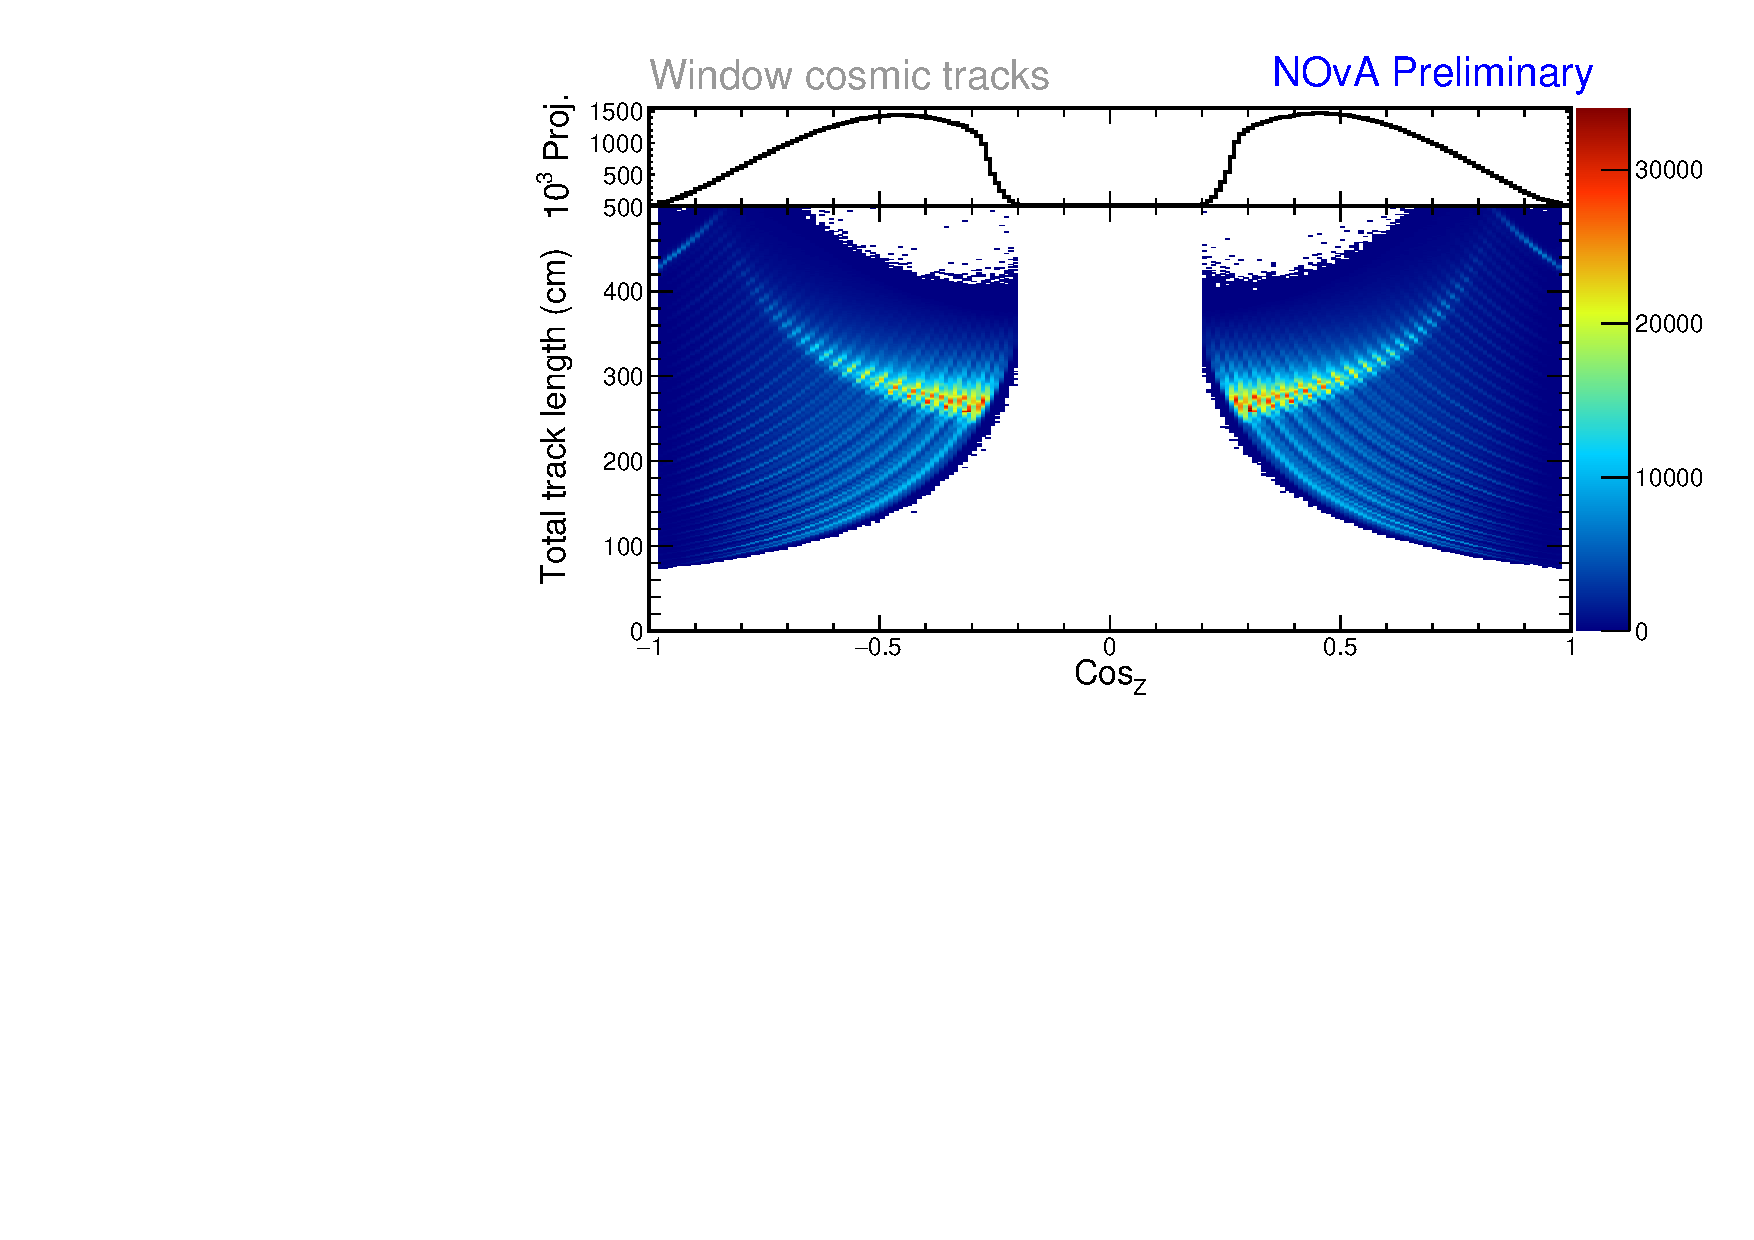
\includegraphics[width=\textwidth]{Plots/TBCalibration/DBSim_BPFPeaks_WTTracks_dcosz_TotLength.pdf}
\caption[Tracking algorithms $\textsf{Cos}_Z$ distributions for the data-based simulation selection]{Investigating the origin of the rugged shape in the $\textsf{Cos}_Z$ distribution of \acrshort{BPF} tracks. The top plot is created with the Loose calibration cuts and the bottom plot with the Full calibration cuts, as described on Tab.~\ref{tab:DataBasedSimEventSelection}. However, this difference in selection shouldn't matter. The long lines on the 2D plots are likely the effects of the detector structure. We can see that for the \acrshort{BPF} tracks, each $\textsf{Cos}_Z$ angle corresponds to a specific track length, whereas for the Window cosmic tracks there is multiple track length for each angle. This could cause the resulting shape in the $\textsf{Cos}_Z$ distribution of \acrshort{BPF} tracks.}
\label{fig:DataBasedSimBPFPeaks}
\end{figure}

\item Second, each reconstruction algorithm has intrinsic deficiencies that can lead to misreconstructions. Applying the full calibration cuts may remove misreconstructed events that should have been included in the simulation, introducing a bias.
\end{enumerate}

To address these concerns, we loosened the full calibration cuts to create a `buffer' around the selected events, allowing for fluctuations of the reconstruction algorithms while maintaining track quality. This way, events that would have been removed based on the calibration cuts applied to their reconstructed \gls{BPF} tracks, but kept based on the calibration cuts applied to their Window cosmic tracks, now have a chance to make it into the final selection and therefore calibration sample. The differences between the full calibration cuts and the employed loosened calibration cuts applied to the \gls{BPF} tracks are listed in Tab.~\ref{tab:DataBasedSimEventSelection} and shown in Fig.~\ref{fig:DataBasedSimTrackComparison}. There we also show the data calibration sample, which was created by applying the full calibration cuts on window cosmic tracks from the same artdaq data sample.
\end{enumerate}

\iffalse
The cuts are:
\begin{itemize}
\item Tracks must have at least two X and two Y cells
\item The difference between the start and stop Z position of the track must be at least 70~cm
\item The Z component of the initial direction vector of the track must be at least 0.2
\item At least 80\% of cells in slice must be reconstructed into the track in both X and Y views
\item At most 6 cells were hit per plane
\item Maximum difference between the first planes in X and Y is 3 (same for the last planes)
\item The difference between number of planes crossed in X and Y view must be at most 10\% of the total number of planes crossed
\item Remove tracks where a step between trajectory points is more than this value * the median step size
\end{itemize}
\fi

\begin{table}[!ht]
\centering
\caption[Overview of the event selection for the data-based simulation]{Event selection of cosmic muons used for the data-based simulation (in green under Loose selection) and comparison to the Full selection cuts used to create the calibration samples in blue. The last two rows are not used for Test Beam, but are employed for the Near and Far detectors and should be examined before creating another data-based simulation for them.}
\begin{tabular}{clcc}
& \multirow{2}{*}{\centering{\textbf{Cut}}} & \multicolumn{2}{c}{\textbf{Selection}}\\
& & \cellcolor[HTML]{3166FF}\textbf{Full} & \cellcolor[HTML]{32CB00}\textbf{Loose}\\\hline
                                   & Muon assumption and 3D track from BPF         &                                             &                                          \\
                                   & Max. track start distance from edge                       & \multicolumn{2}{c}{50 cm}                                                                 \\
                                   & Max. $Cos_{Z}$                                            & \multicolumn{2}{c}{0.98}                                                               \\ \hline
                                   & Max. number of hits in X or Y                             & \multicolumn{2}{c}{\cellcolor[HTML]{FFFFFF}2}                                          \\
                                   & Min. difference between Stop$_{Z}$ and Start$_{Z}$        & \cellcolor[HTML]{3166FF}70~cm                 & \cellcolor[HTML]{32CB00}50~cm             \\
                                   & Min. $Cos_{Z}$ & \cellcolor[HTML]{3166FF}0.2                 & \cellcolor[HTML]{32CB00}0.15             \\
                                   & Min. frac. of slice hits in track in each view    & \multicolumn{2}{c}{0.8}                                                                \\
                                   & Max. number of cells per plane in each view               & \cellcolor[HTML]{3166FF}6                   & \cellcolor[HTML]{32CB00}15               \\
                                   & Max. difference in X-Y for first (last) plane     & \cellcolor[HTML]{3166FF}3                   & \cellcolor[HTML]{32CB00}5                \\
                                   & Max. plane asymmetry                                      & \cellcolor[HTML]{3166FF}0.1                 & \cellcolor[HTML]{32CB00}0.2              \\
                                   & Max. step size to median step size ratio                  & \cellcolor[HTML]{3166FF}3                   & \cellcolor[HTML]{32CB00}5                \\
                                   & \cellcolor[HTML]{C0C0C0}Max. vertex distance from edge    & \multicolumn{2}{c}{\cellcolor[HTML]{C0C0C0}10~cm}                                         \\
\parbox[t]{2mm}{\multirow{-10}{*}{\rotatebox[origin=c]{90}{Calibration sample selection}}}& \cellcolor[HTML]{C0C0C0}Max. track end distance from edge & \multicolumn{2}{c}{\cellcolor[HTML]{C0C0C0}10 cm}
\end{tabular}
\label{tab:DataBasedSimEventSelection}
\end{table}

\begin{figure}[!h]
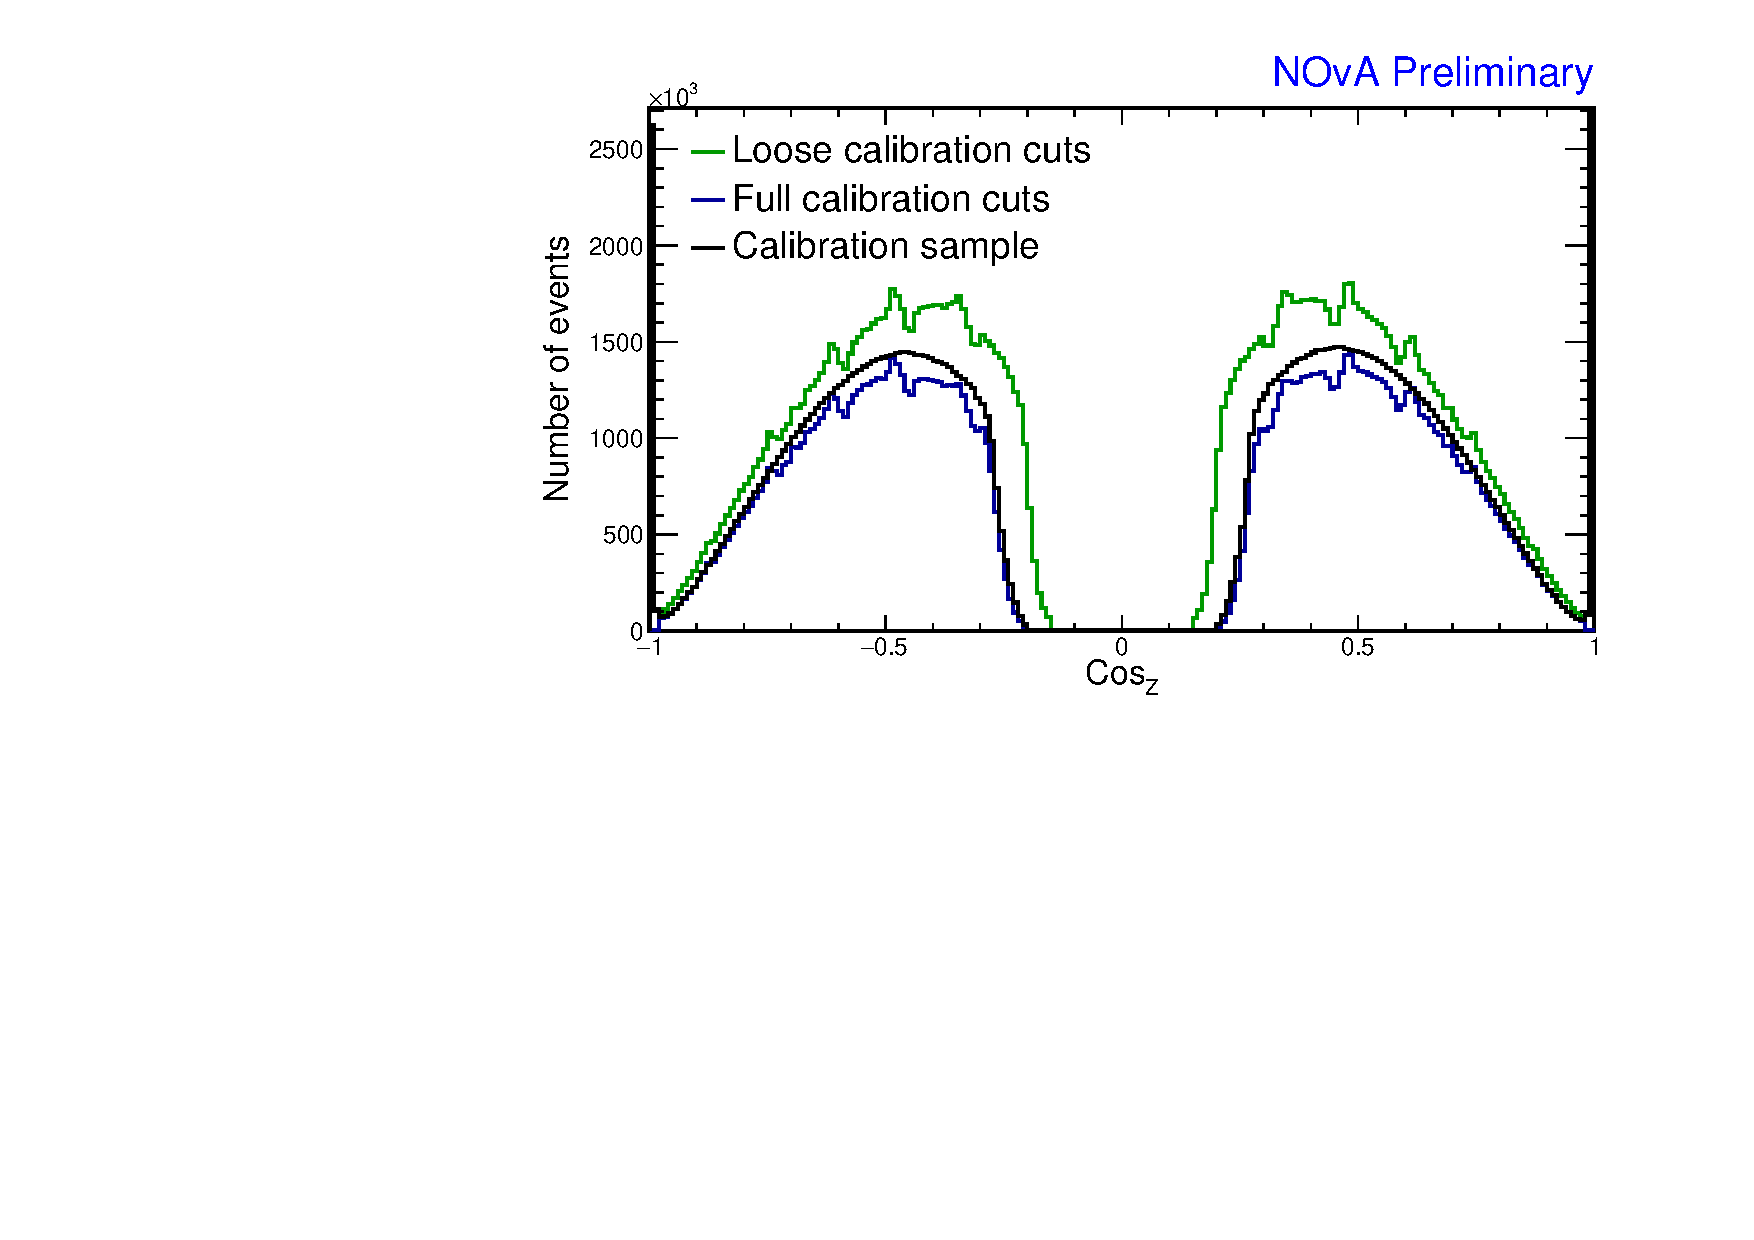
\includegraphics[clip, width=\textwidth]{Plots/TBCalibration/DBSim_SelectionComparisonPCHitsListCut_CosZ.pdf}
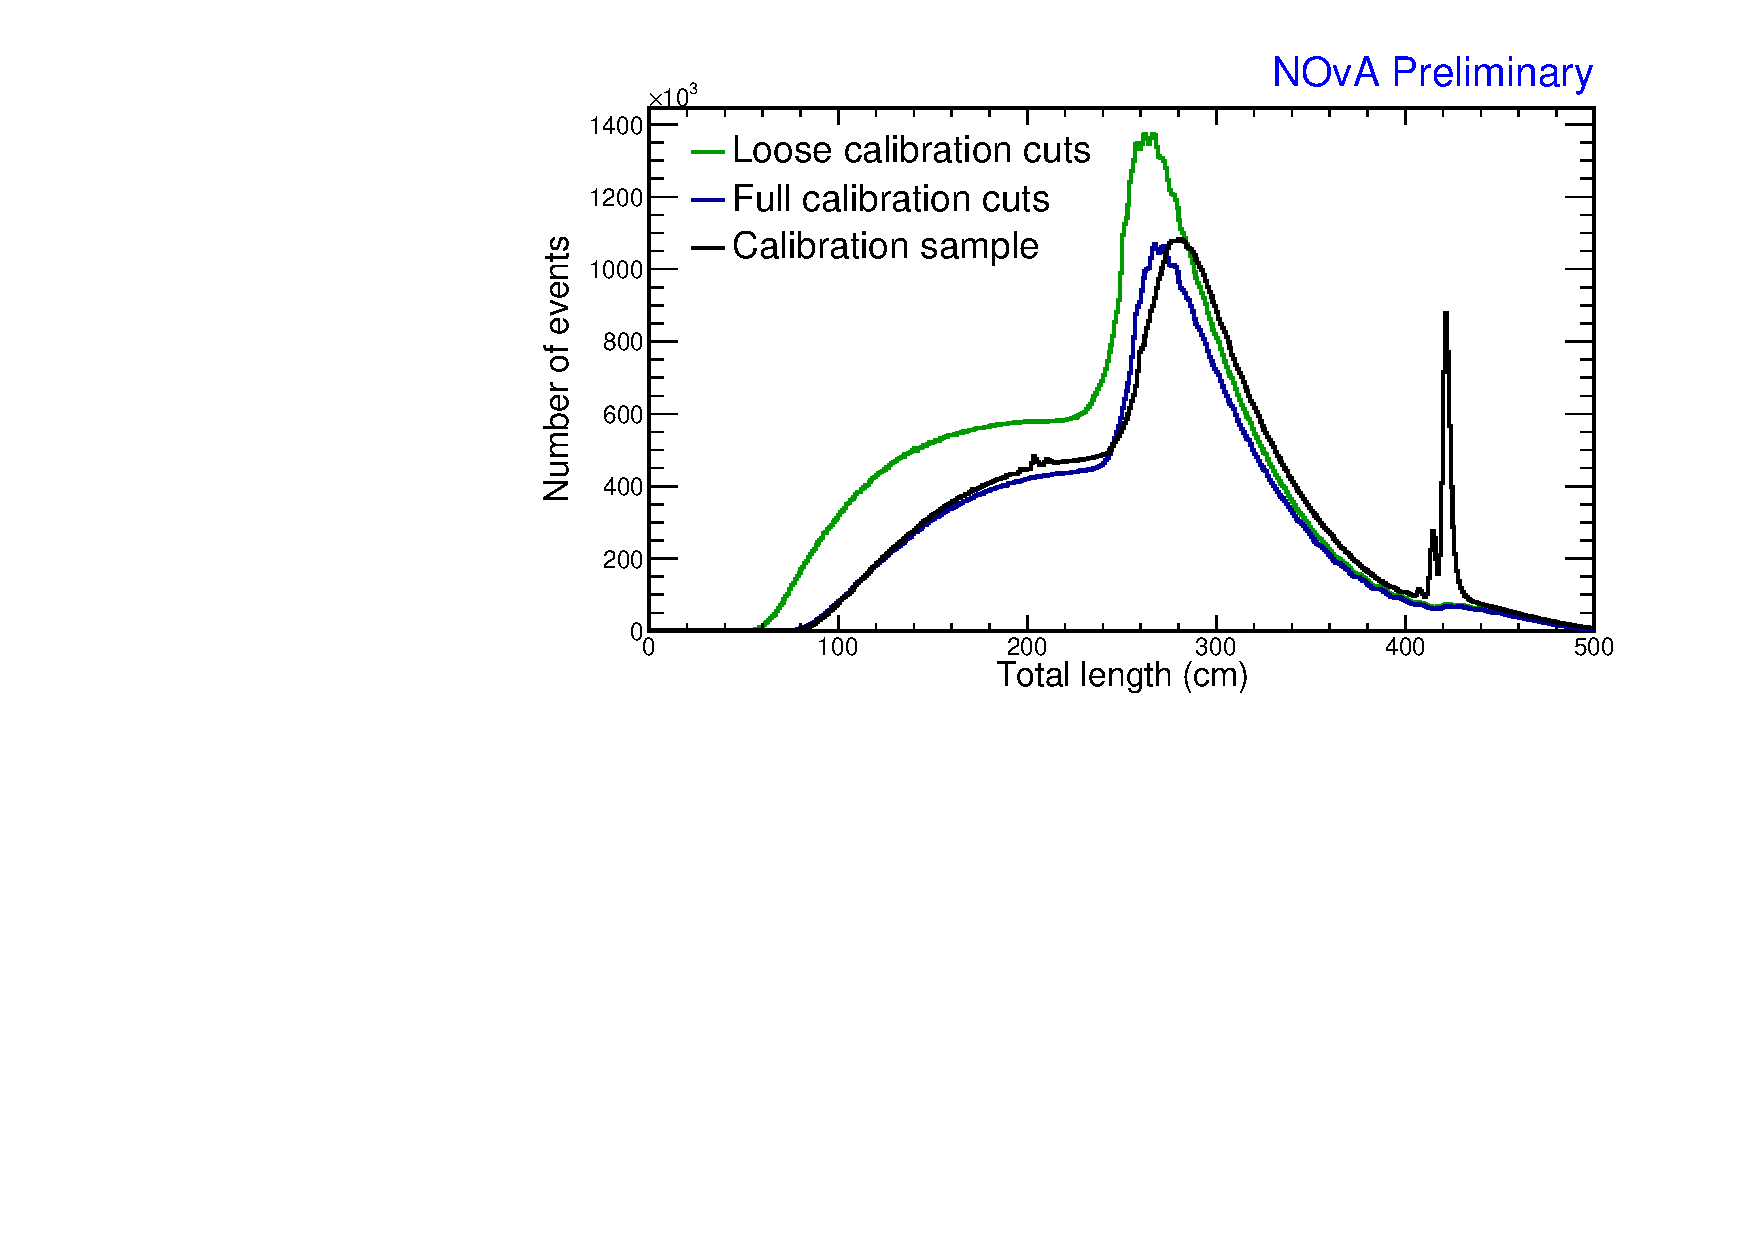
\includegraphics[clip, width=\textwidth]{Plots/TBCalibration/DBSim_SelectionComparisonPCHitsListCut_TotLength.pdf}
\caption[Event selection for the data-based simulation]{Comparison of event selections for the data-based simulation and of the corresponding data calibration sample in black. The green line represents the final selection used for the simulation, using the loosened calibration cuts, as describe in text and in Tab.~\ref{tab:DataBasedSimEventSelection}. The blue line shows the distributions with full calibration cuts applied to the same sample and using the same tracks. The `calibration sample' shown in black was made with the same full calibration cuts as the blue line (without the track start cut and maximum Cos$_Z$ cuts), but applied to the window cosmic tracks instead of the \acrshort{BPF} tracks. All of the distributions are made from the period 4 Test Beam data.}
\label{figPCHitsListCutsComparison}
\end{figure}

During the selection process, we determine whether the muon is stopping inside the detector or passing through, based on the reconstructed track's end position. For Test Beam we say it is a stopping muon if its track ends at least $\unit[20]{cm}$ from any edge of the detector. For the far and near detector this is $\unit[50]{cm}$. This information assists in correcting the energy of through-going muons, as outlined in the following Sec.~\ref{sec:DataBasedSimPython}.

%\FloatBarrier
\subsection{Energy Correction, Charge Assignment and Smearing}\label{sec:DataBasedSimPython}
Once we have the kinematic information for the selected events, we perform several tasks to get the final sample of cosmic muon events for the data-based simulation. This includes correcting energies of the through-going muons, assigning a charge to each muon event, and smearing and converting the information into the correct format required by the generator.

\subsubsection*{Energy Correction}
Through-going muons do not deposit all of their energy inside the detector. From the reconstructed information we cannot reliably calculate their initial energies, but we can estimate an energy that could leave the same track. In general, the energy spectrum of cosmic muons can be approximately described by a power law $E^{-\alpha}$, with $\alpha\approx2.7$ \cite{NOvA-doc-51327,rpp2022-rev-cosmic-rays.pdf}. The expectation value for the `true' initial energy of through-going muons can be therefore calculated as
\begin{equation}
\left\langle E\right\rangle =\frac{\int^{E_C}_{E_R} E\cdot E^{-\alpha}}{\int^{E_C}_{E_R} E^{-\alpha}}=\left(\frac{\alpha -1}{\alpha -2}\right)\left(\frac{E_C^{2-\alpha}-E_R^{2-\alpha}}{E_C^{1-\alpha}-E_R^{1-\alpha}}\right),
\end{equation}
where $E_R$ is the reconstructed energy we got from the \gls{BPF}. $E_C$ is the critical energy chosen to be $\unit[300]{GeV}$, as we do not expect muons with higher energies to be selected due to large showers along their paths.

We use this corrected initial energy for all muons that do not stop inside the detector, as identified during selection described in Sec.~\ref{sec:DataBasedSimSelection}. Figure \ref{fig:DataBasedSimEnergyScaling} shows the corrected energy distribution of our selected events and demonstrates that the choice of the critical energy does not significantly change the correction. 

\begin{figure}[hbtp]
\centering
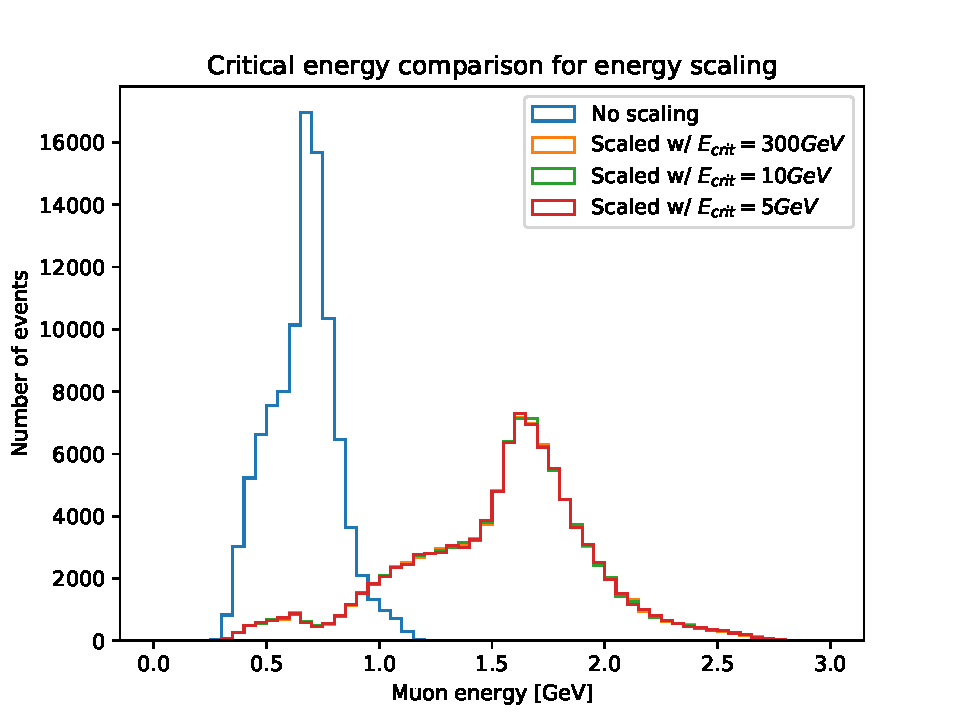
\includegraphics[width=0.8\textwidth]{Plots/TBCalibration/DBSim_ECritComparison.pdf}
\caption[Energy correction for through-going muons for the data-based simulation]{The effect of energy correction for through-going muons with various critical energies. No significant difference can be seen when using different critical energies.}
\label{fig:DataBasedSimEnergyScaling}
\end{figure}

This corrected energy is \textbf{not} a good representation of the true energy spectrum of cosmic muons on surface level and getting a correct energy distribution from data would require a much more dedicated effort. The corrected energy would also be different for different \gls{NOvA} detectors, since the reconstructed energy is calculated from the track length. For example, the corrected energy of cosmic muons when entering the detector would be larger for the bigger \gls{ND} than for Test Beam, even though the \gls{ND} is underground. 

However, since this simulation is intended to be used for calibration, where we use through-going muons only for relative calibration, we do not need a perfect representation of the cosmic muon energy spectrum. Not including more energetic cosmic muons into the simulation does bias the energy deposition towards lower values, but this is corrected for during absolute calibration which only uses stopping muons, for which we assume we reconstruct their energy well from \gls{BPF}.

If someone were to use this simulation for something other than calibration, it would be necessary to rethink the energy correction, either by changing the energy estimation from track based algorithms to energy deposition, or by including information from external sources. It would also be necessary to include angular dependence for the energy correction as described in the PDG \cite{rpp2022-rev-cosmic-rays.pdf}.

\subsubsection*{Smearing}
The reconstructed data is influenced by the detector structure, reconstruction efficiencies and other effects that can bias the simulation. To avoid this influence, we smear the reconstructed values by randomly changing
\begin{itemize}
\item the total momentum within 2\%,
\item the azimuthal angle uniformly,
\item the polar angle within $\unit[4]{mrad}$,
\item and the X/Y and Z vertex positions within the width or depth of the cell respectively.
\end{itemize}

The size of the smearing has been decided as the best estimate of variations of these variables for cosmic muons.

\subsubsection*{Charge Assignment}
We need to tell the detector simulation whether to simulate a muon or an anti-muon. However we do not reconstruct the charge of the muons, so we have to randomly assign it based on a statistical distribution from external measurements \cite{NOvA-doc-51327}:

%Figure out where are the plots and the equation Mark/Teresa quoted from (somewhere in PDG). Describe the basis of the measurement.
%Here(p10): https://pdg.lbl.gov/2022/reviews/rpp2022-rev-cosmic-rays.pdf
%But the equation must be from one of the sources listed.

\begin{equation}
P_+ \simeq 0.539 + \frac{x}{34.5}-\left(\frac{x}{9.48}\right)^2 + \left(\frac{x}{8.27}\right)^3,
\end{equation}
where $x$ is the logarithm of the total momentum in $\unit{GeV}$.

\subsubsection*{Running the Simulation}
We save the vertex positions, the four momenta and the assigned charge into a text file, that is then fed into the same detector and readout simulation chain, as was described for the \gls{ND} and \gls{FD} in Sec.~\ref{sec:NOvASimulation}.  We use the fibre brightness map that is used in calibration (see Sec.~\ref{sec:NOvACalibration}) to inform the simulation about the real detector conditions. Since we want the simulated detectors to be functional copies of the ideal versions of the real detectors, it is important to provide a correct brightness file without any defects. For this simulation we use the fibre brightness map described in Sec.~\ref{sec:FibreBrightnessTB}.

\subsection{Validation}
To validate whether the newly created simulation works as expected, we compare the new simulation with the original data it was created from. Additionally, we use the new simulation as `fake data' and pass the simulated events through the same reconstruction, selection and simulation processes as were used to create the first simulation, creating a `re-simulation' sample. This is used to validate the stability of the simulation process.

For the data-simulation comparisons we use the events from the actual calibration samples as data. This is equivalent to looking at the Window cosmic tracks with full calibration cuts described in the selection Sec.~\ref{sec:DataBasedSimSelection}. We are expecting the new simulation to be similar to the data calibration sample, without a bias from the original data used for the simulation.

Figures \ref{fig:DataBasedSimDataMCComparison_cosXcosY} and \ref{fig:DataBasedSimDataMCComparison_cosZtotLength} show that the angular distributions of the new simulation (pink lines) are almost the same as the distributions of the \gls{BPF} tracks with full calibration cuts (blue dashed lines). This means that loosening up the calibration cuts (green dashed lines) did not help as expected with compensating for the underlying differences between the \gls{BPF} tracks and the Window cosmic tracks. This can also be seen on the total track length distribution in Fig.~\ref{fig:DataBasedSimDataMCComparison_cosZtotLength}. During the development of the event selection we created three more versions of the simulation with various event selections, including with full calibration cuts and with different loosened calibration cut values. It became clear that it is unlikely we could mitigate these track algorithm differences by changing the selection even more. Since the entire simulation process is fairly time and resource consuming and the distributions of the new simulation look reasonable and are close enough to the data, we've decided to proceed with this version of the simulation and use it in the Test Beam calibration.

\begin{figure}[!ht]
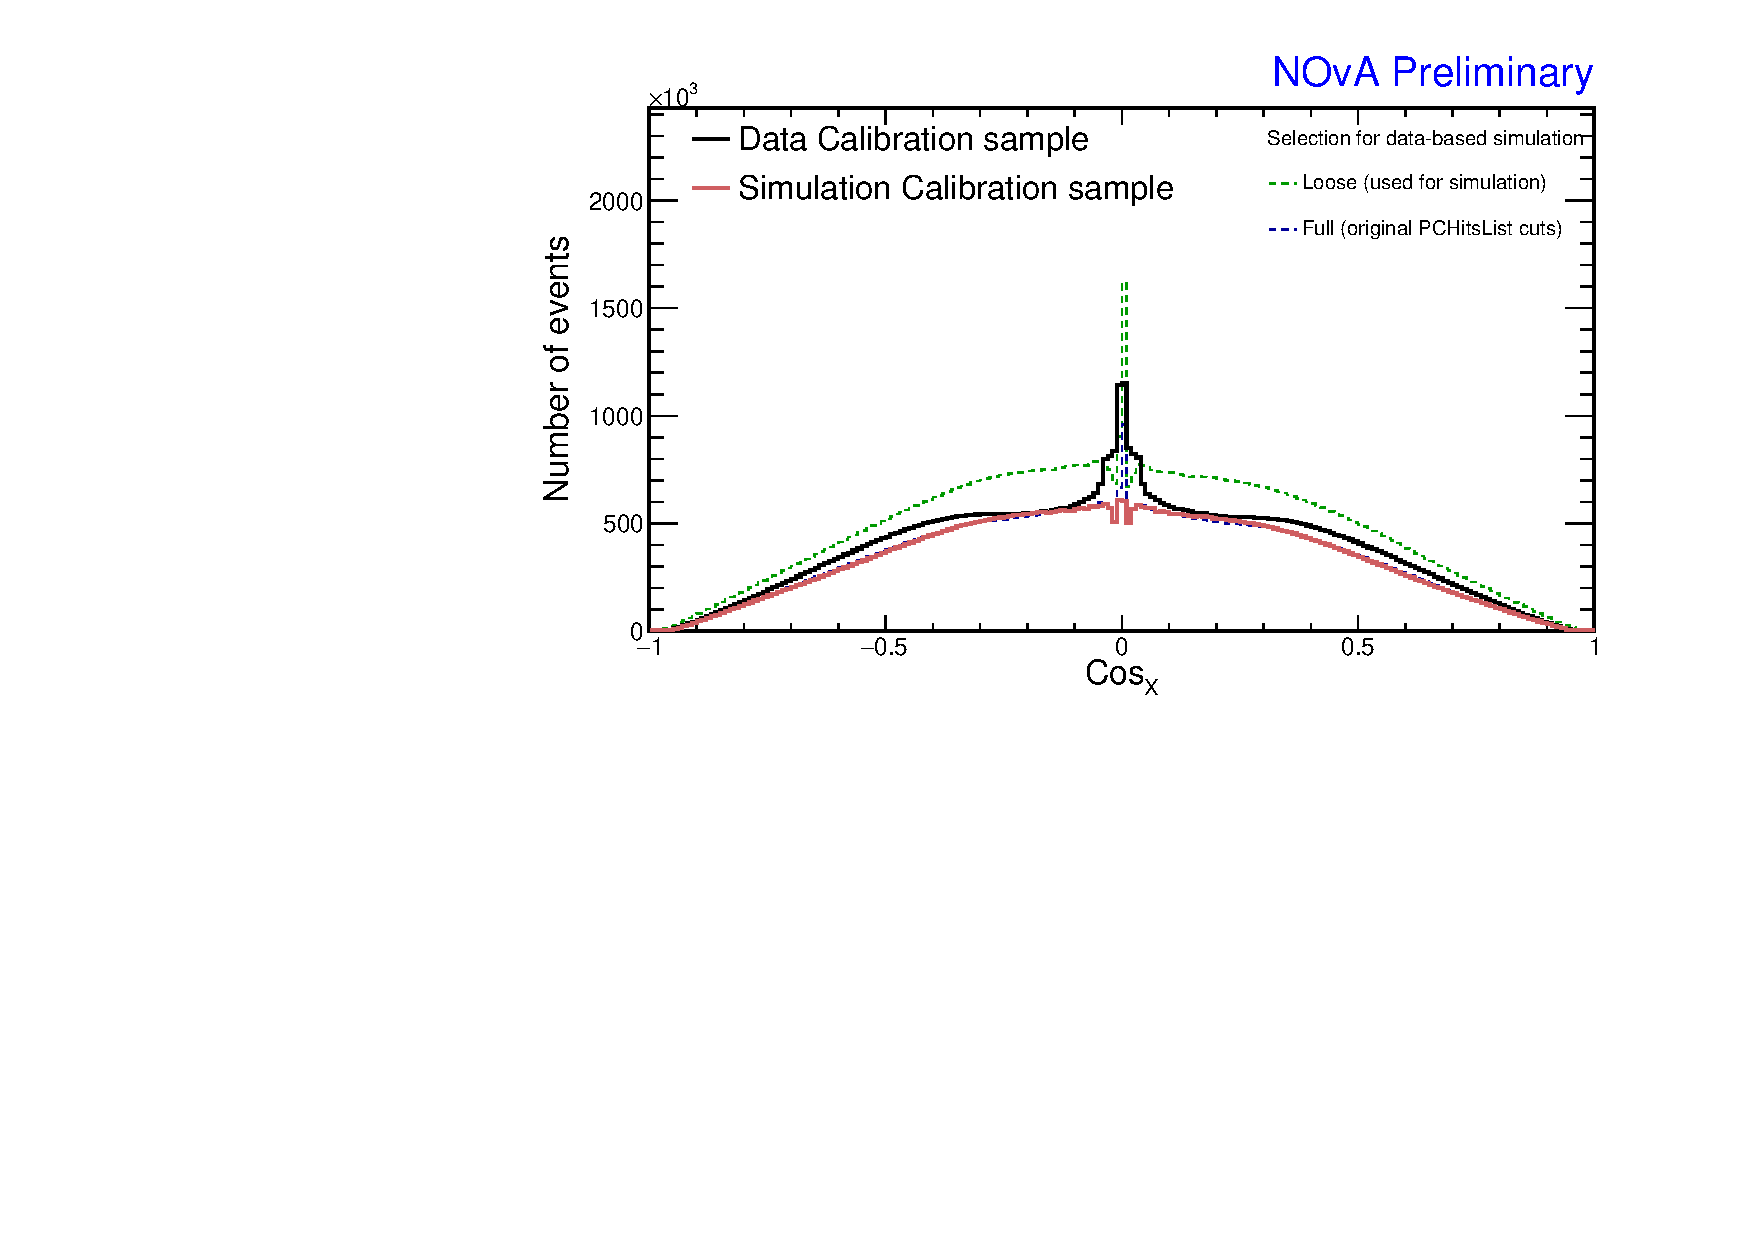
\includegraphics[width=\textwidth]{Plots/TBCalibration/DBSim_DataMCComparison_CosX.pdf}
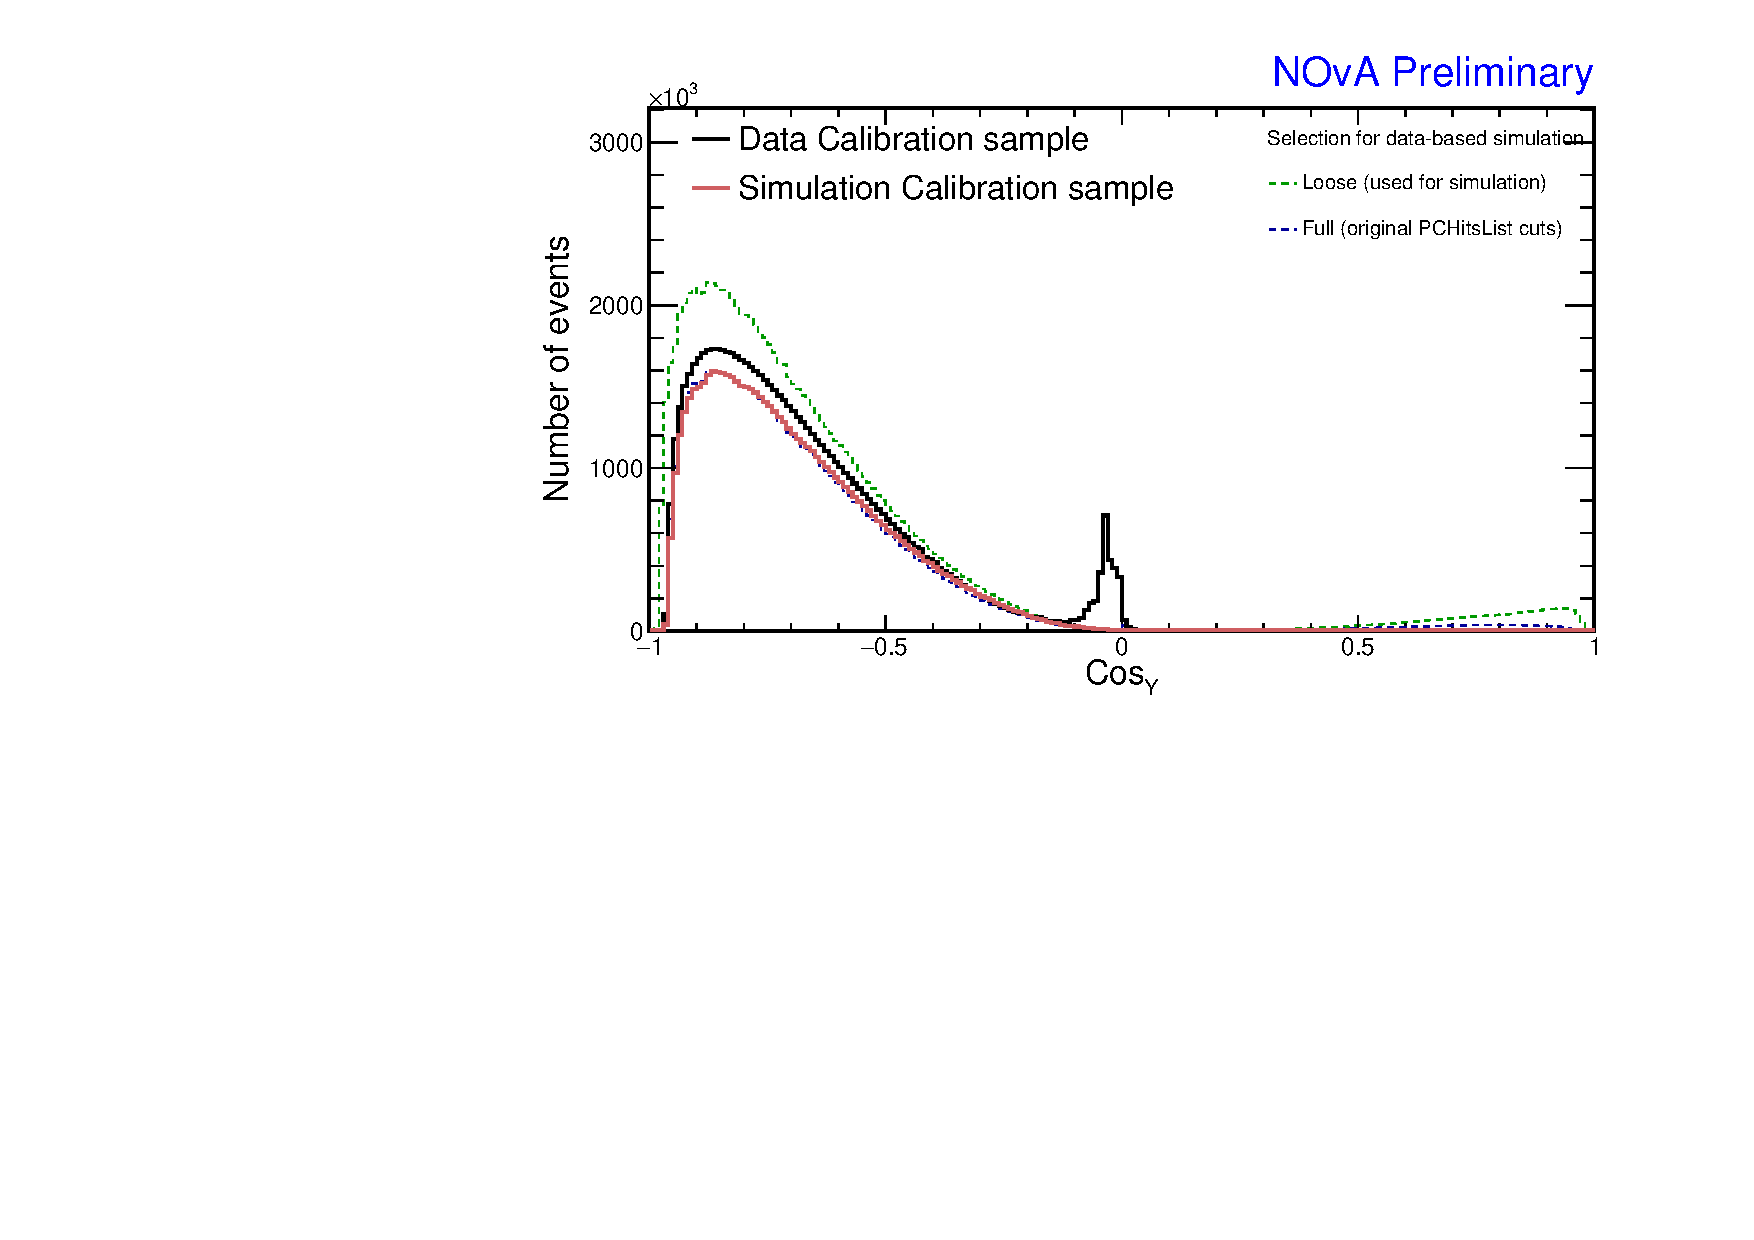
\includegraphics[width=\textwidth]{Plots/TBCalibration/DBSim_DataMCComparison_CosY.pdf}
\caption[Data-Simulation comparison of angular distributions]{Angular distribution comparison of the newly created simulation calibration sample and the corresponding data calibration sample. We are also showing the selection of data used to create the new simulation in green and a `full calibration cuts' selection (same cuts as used for the simulation calibration sample but applied to \acrshort{BPF} tracks instead of Window cosmic tracks) in blue.}
\label{fig:DataBasedSimDataMCComparison_cosXcosY}
\end{figure}

\begin{figure}[!ht]
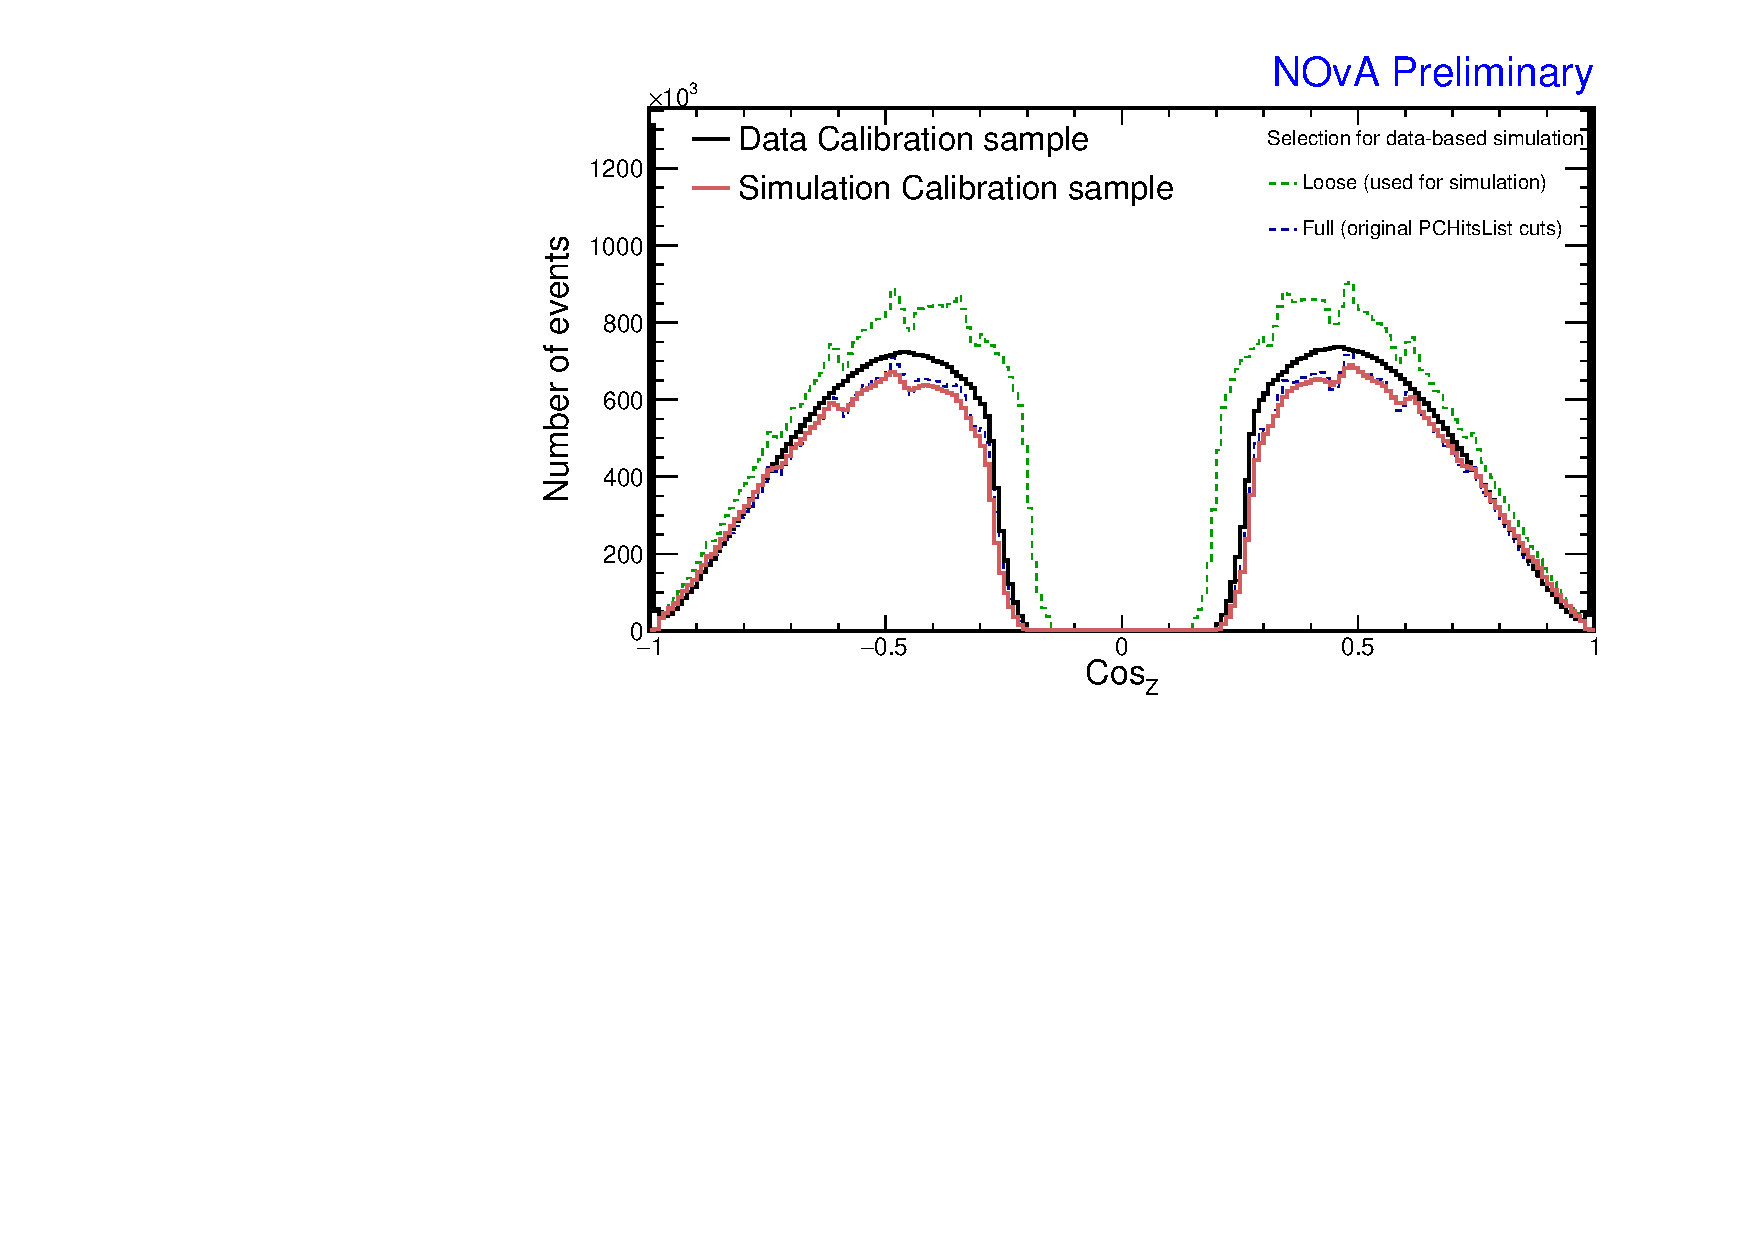
\includegraphics[width=\textwidth]{Plots/TBCalibration/DBSim_DataMCComparison_CosZ.pdf}
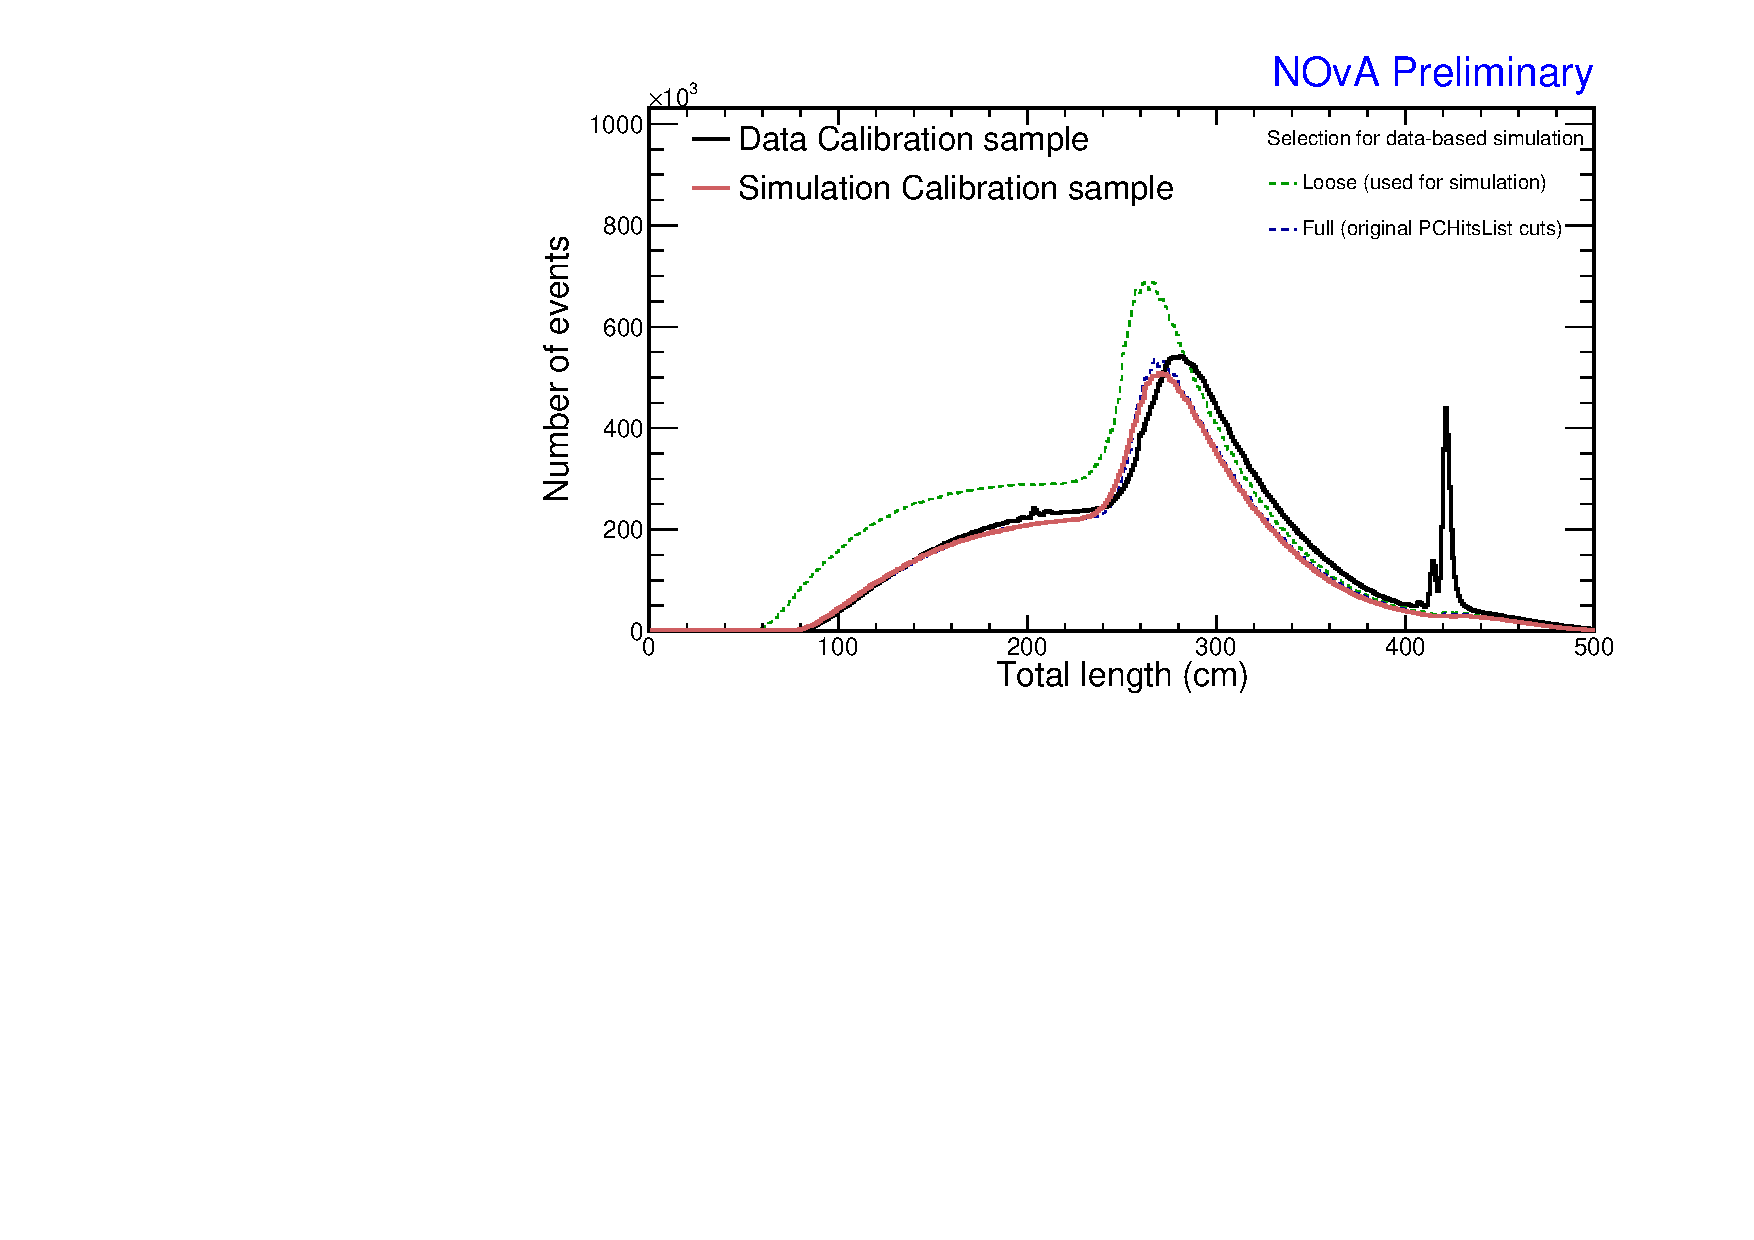
\includegraphics[width=\textwidth]{Plots/TBCalibration/DBSim_DataMCComparison_TotLength.pdf}
\caption[Data-Simulation comparison of angular and track length distributions]{Angular and total track length distribution comparison of the newly created simulation calibration sample and the corresponding data calibration sample. We are also showing the selection of data used to create the new simulation in green and a `full calibration cuts' selection (same cuts as used for the simulation calibration sample but applied to \acrshort{BPF} tracks instead of Window cosmic tracks) in blue.}
\label{fig:DataBasedSimDataMCComparison_cosZtotLength}
\end{figure}

The start of track comparison between data and simulation in Fig.~\ref{fig:DataBasedSimDataMCComparison_startXstartY} and \ref{fig:DataBasedSimDataMCComparison_startZ} show that there are fewer events that start at the edge of the detector and the vertex positions are moved slightly towards the inside of the detector. This is likely the result of the smearing of the vertex positions and we do not expect this to have an effect on the calibration. \note{Should this have been mitigated? Should I mention here that the smearing is still a good idea?}

\begin{figure}[!ht]
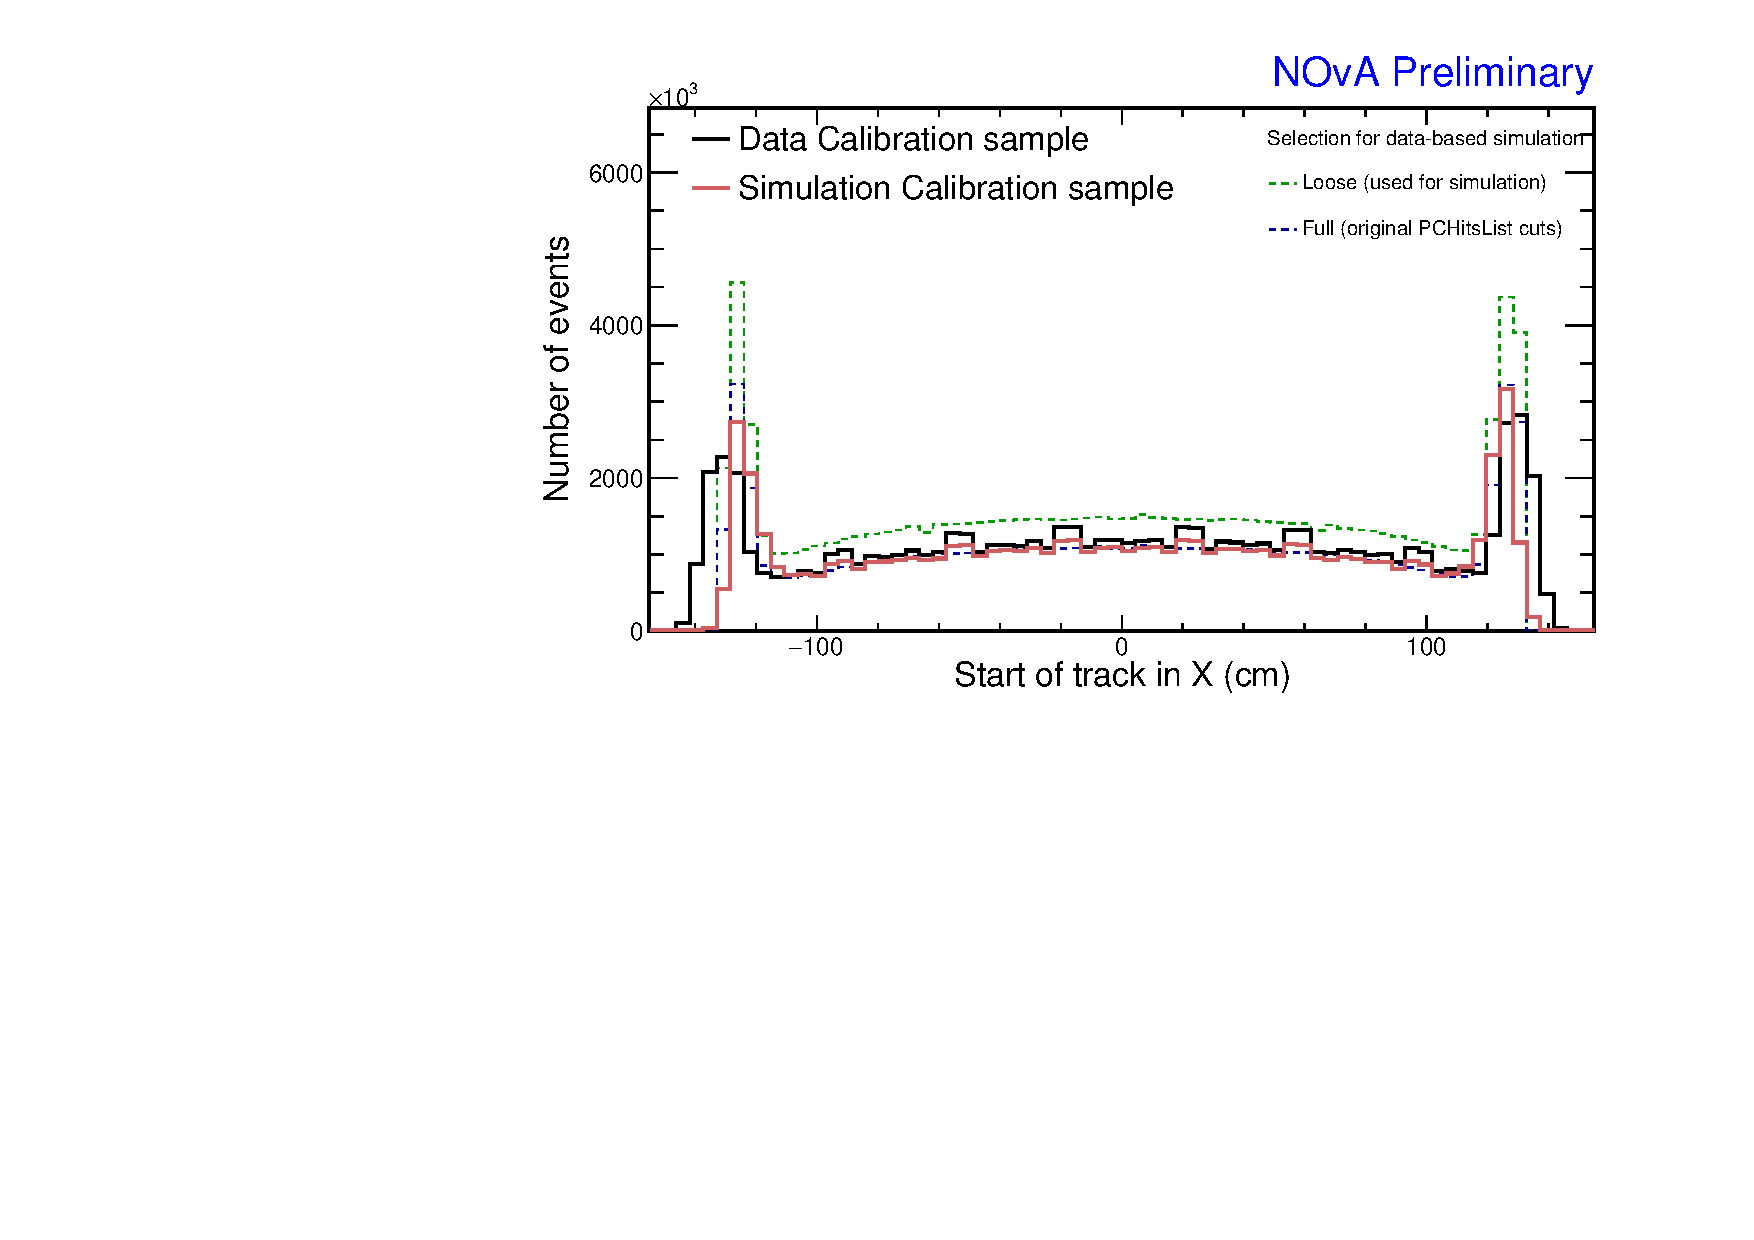
\includegraphics[width=\textwidth]{Plots/TBCalibration/DBSim_DataMCComparison_StartX.pdf}
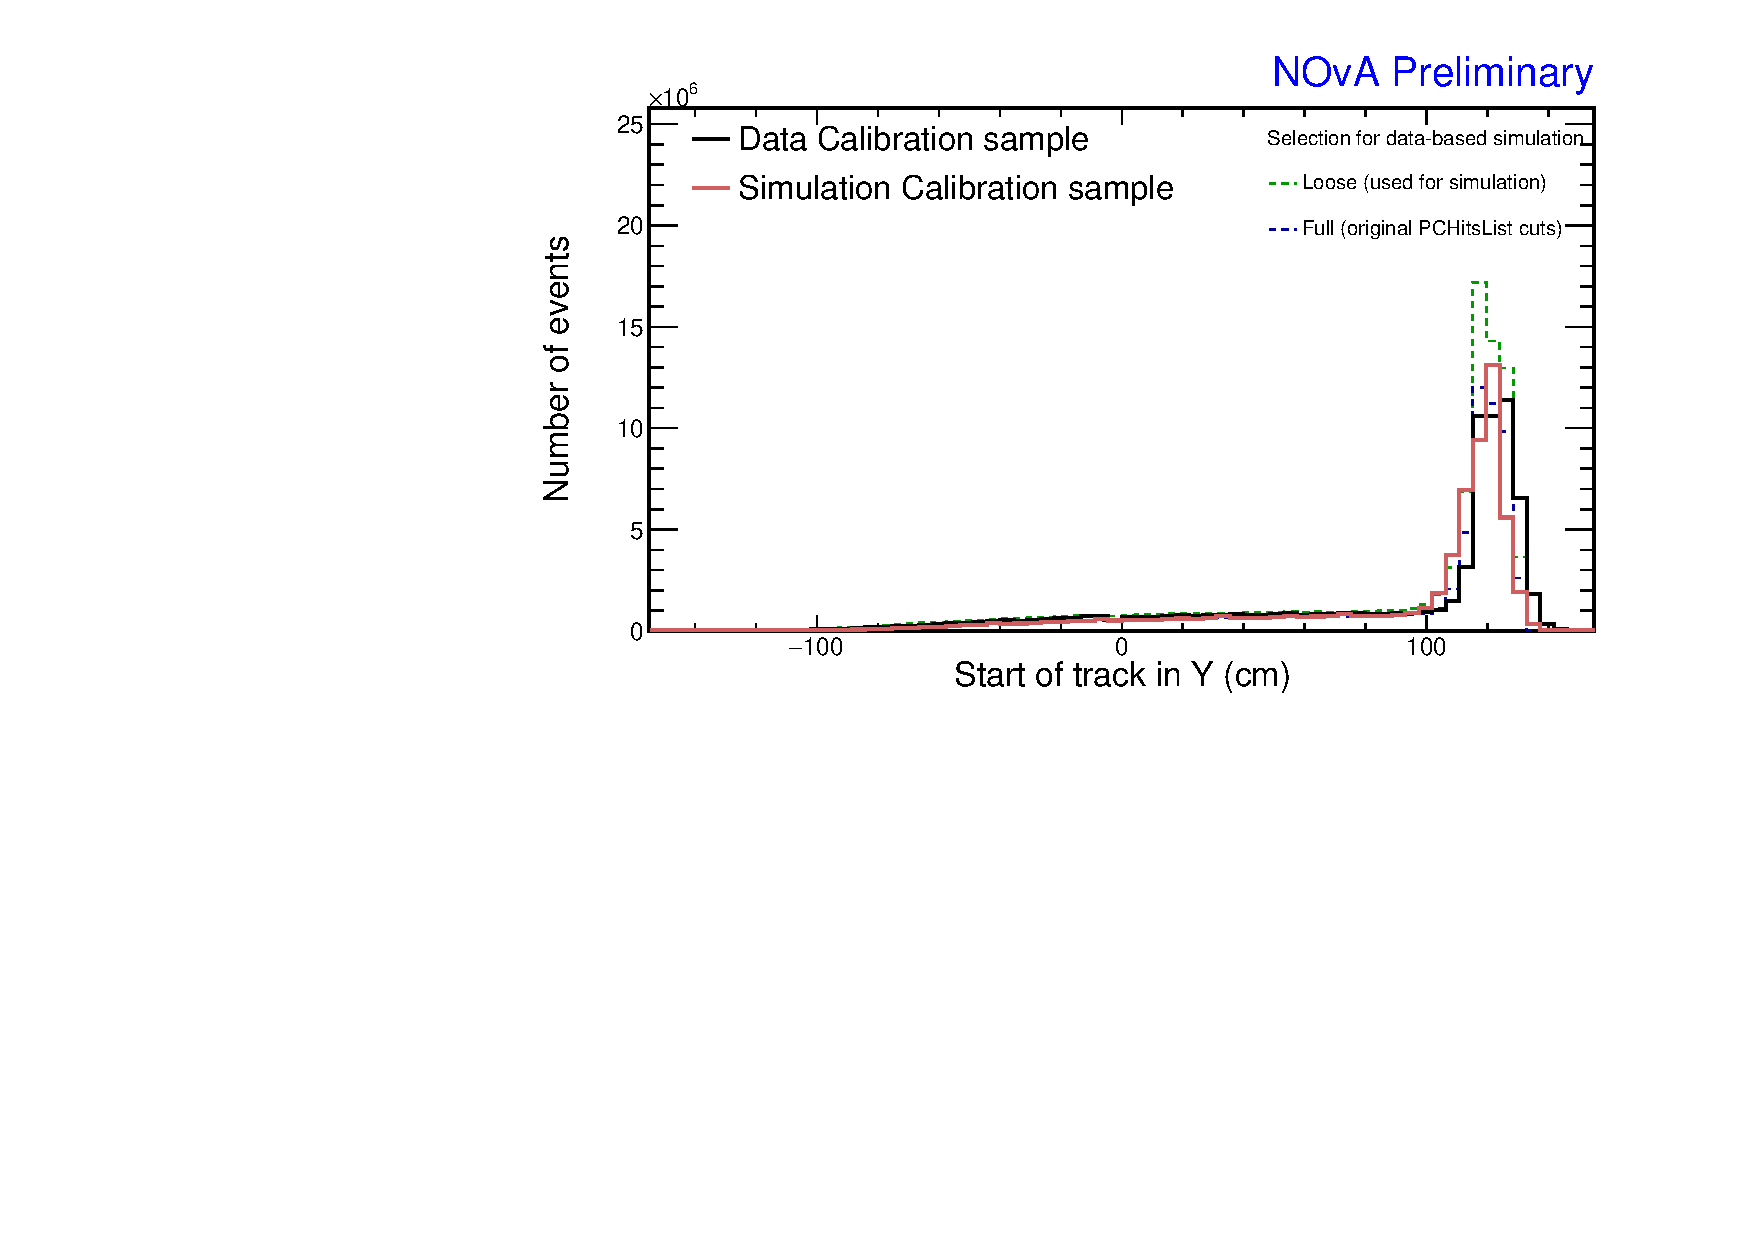
\includegraphics[width=\textwidth]{Plots/TBCalibration/DBSim_DataMCComparison_StartY.pdf}
\caption[Data-Simulation comparison of track start distributions]{Start of tracks comparison of the newly created simulation calibration sample and the corresponding (period 4) data calibration sample. We are also showing the selection of data used to create the new simulation in green and a `full calibration cuts' selection (same cuts as used for the simulation calibration sample but applied to \acrshort{BPF} tracks instead of Window cosmic tracks) in blue.}
\label{fig:DataBasedSimDataMCComparison_startXstartY}
\end{figure}

\begin{figure}[!ht]
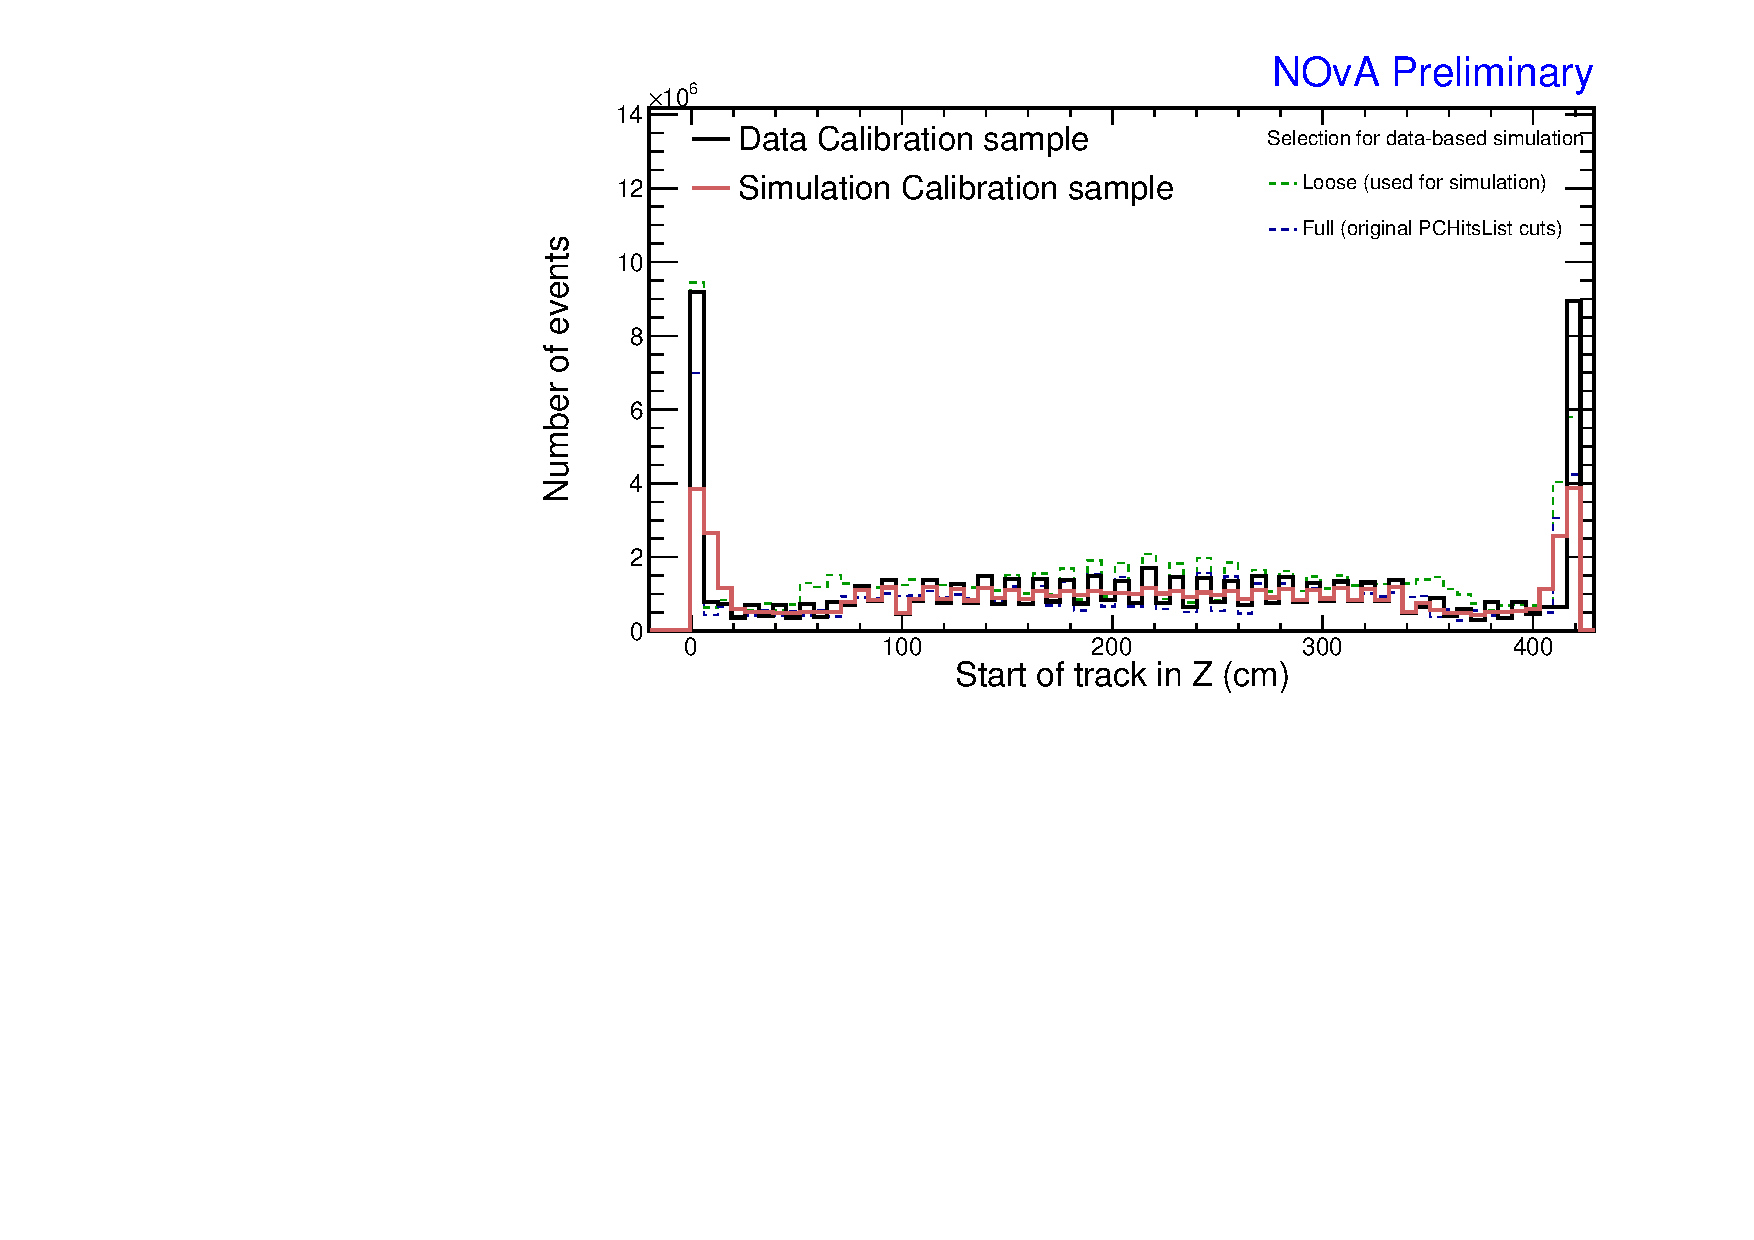
\includegraphics[clip, width=\textwidth]{Plots/TBCalibration/DBSim_DataMCComparison_StartZ.pdf}
\caption[Data-Simulation comparison of track start distribution]{Start of tracks comparison of the newly created simulation calibration sample and the corresponding (period 4) data calibration sample. We are also showing the selection of data used to create the new simulation in green and a `full calibration cuts' selection (same cuts as used for the simulation calibration sample but applied to \acrshort{BPF} tracks instead of Window cosmic tracks) in blue.}
\label{fig:DataBasedSimDataMCComparison_startZ}
\end{figure}

After adding the distributions for the re-simulation calibration sample, shown in Fig.~\ref{fig:DataBasedSimSimVersionComparison}, we can see that the tracks' starts are shifted even further towards the inside of the detector. This would support the hypothesis that this effect is caused by the smearing of the reconstructed variables. This is also likely directly related to the loss of events with longer track lengths as shown in Fig.~\ref{fig:DataBasedSimSimVersionComparison}. If tracks start a few centimetres later in the detector their tracks would get shorter by the same amount.

\begin{figure}[!ht]
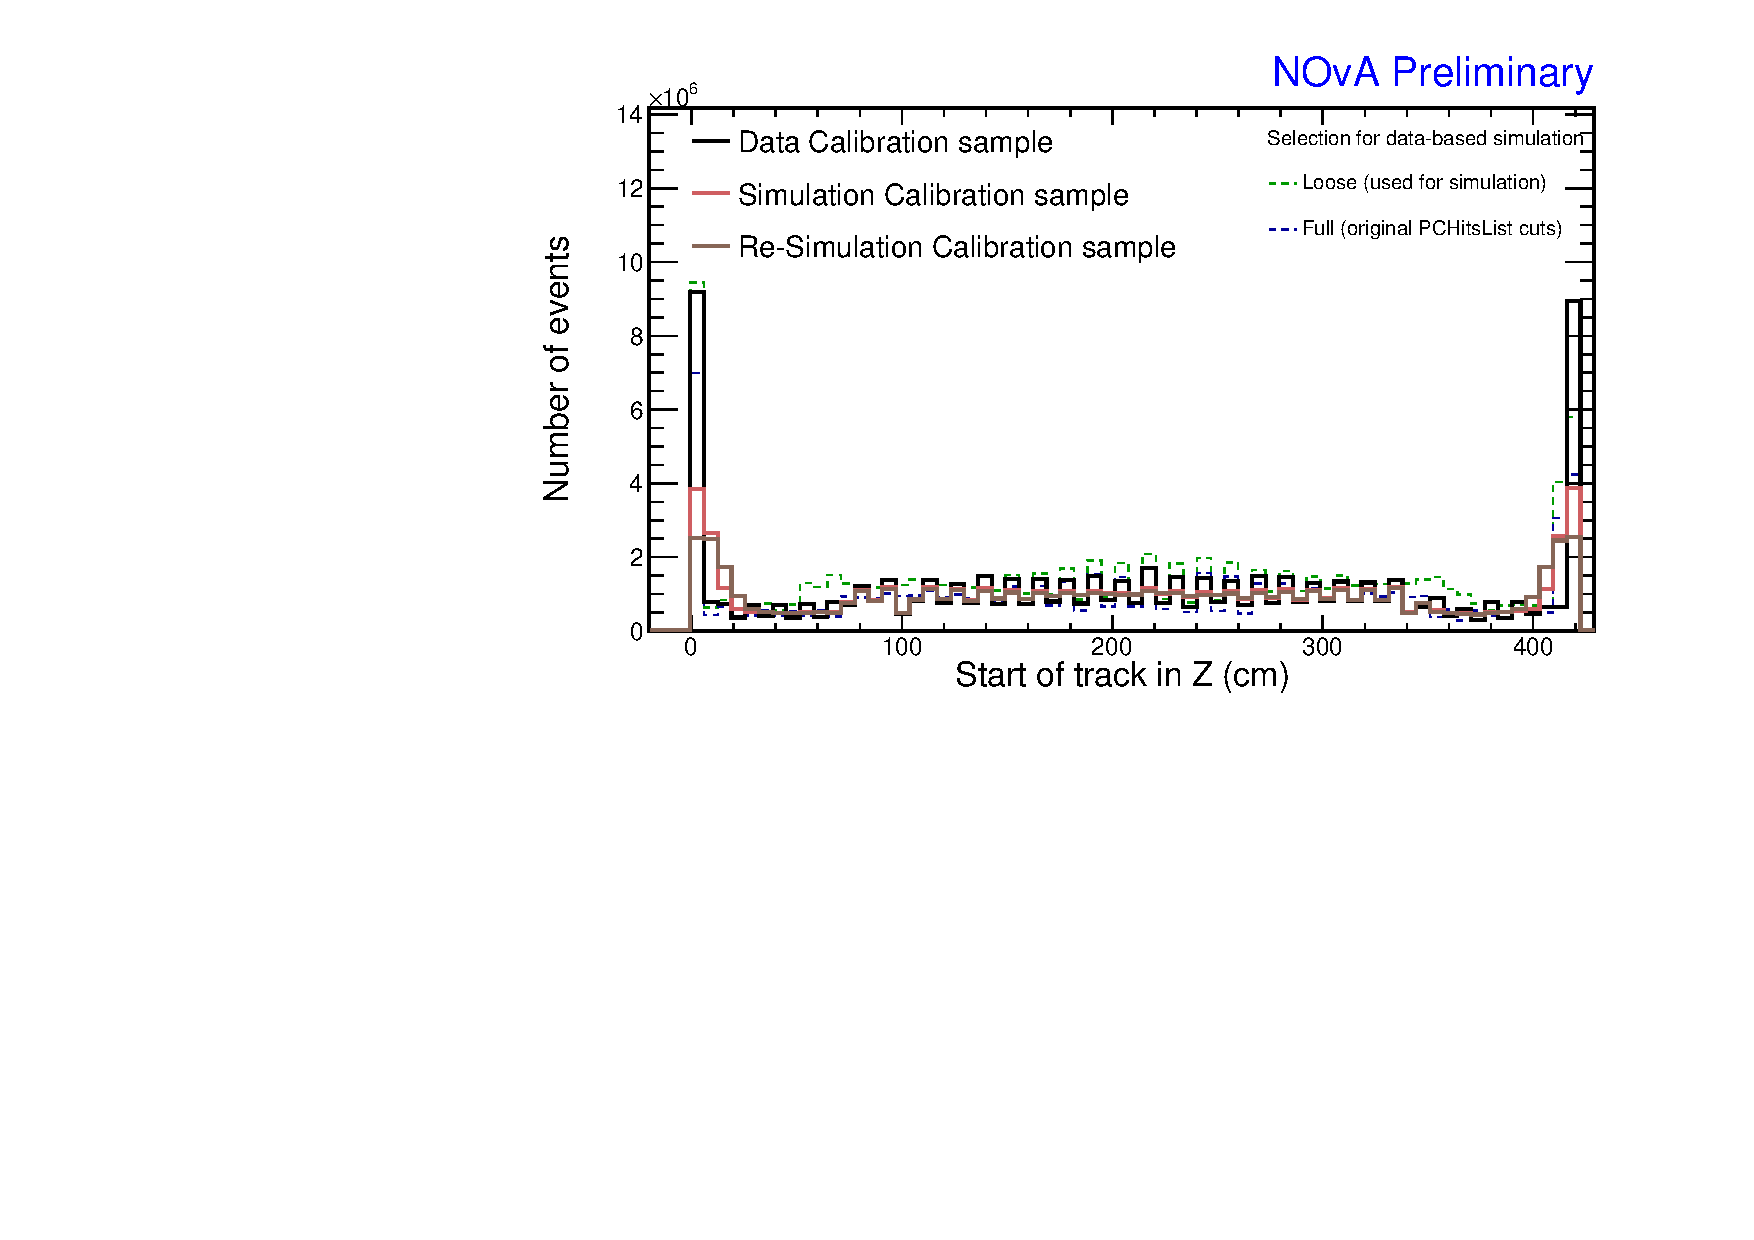
\includegraphics[width=\textwidth]{Plots/TBCalibration/DBSim_SimVersionComparison_StartZ.pdf}
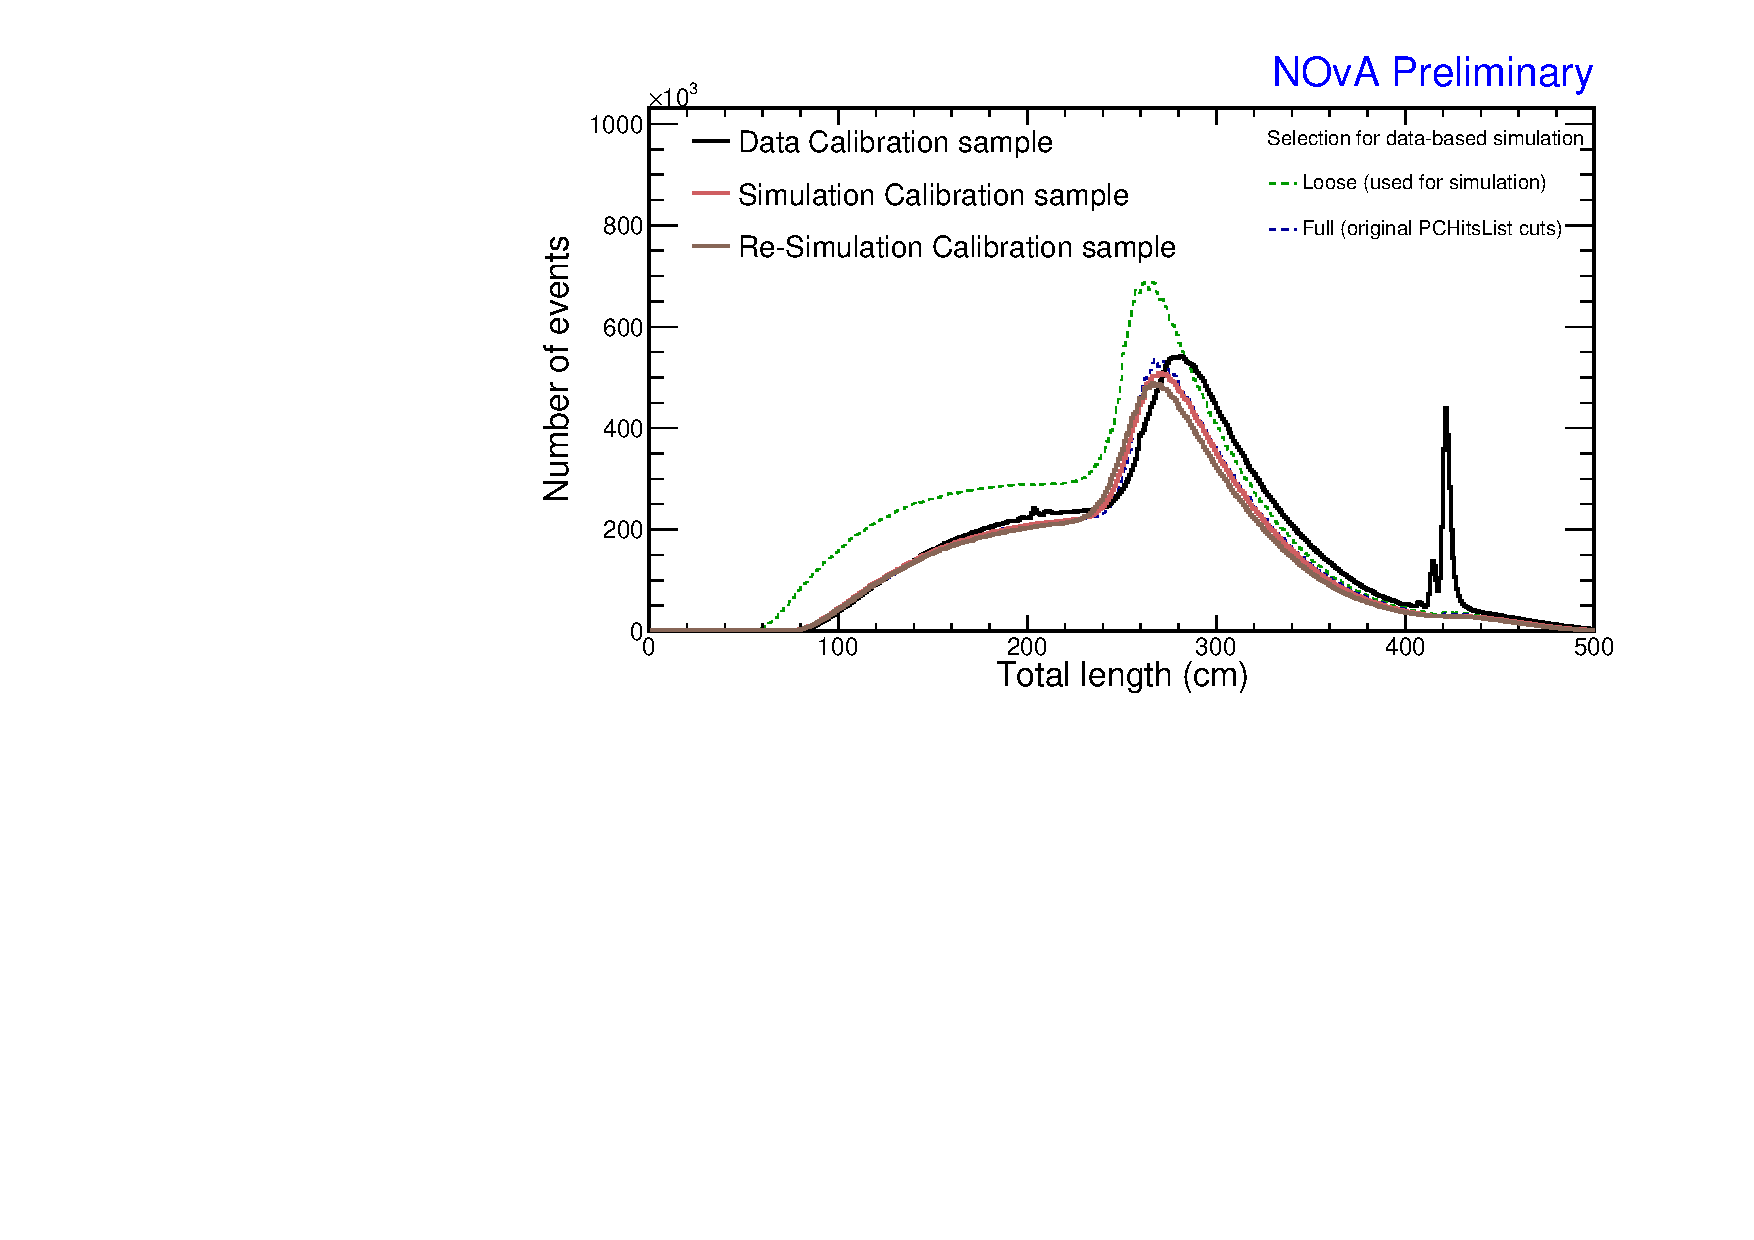
\includegraphics[width=\textwidth]{Plots/TBCalibration/DBSim_SimVersionComparison_TotLength.pdf}
\caption[Comparison of simulation to a circular re-simulation validation sample]{Distribution of the re-simulated events, when the new simulation is used as `fake data' for a new iteration of the simulation process discussed in this document. This is compared to the newly created simulation calibration sample and the corresponding data calibration sample. We are also showing the selection of data used to create the new simulation in green and a `full calibration cuts' selection (same cuts as used for the simulation calibration sample but applied to \acrshort{BPF} tracks instead of Window cosmic tracks) in blue.}
\label{fig:DataBasedSimSimVersionComparison}
\end{figure}

\note{Should I describe every single aspect of the validation plots in here? For example the black peaks in Fig.~\ref{fig:DataBasedSimDataMCComparison_cosXcosY} and \ref{fig:DataBasedSimDataMCComparison_cosZtotLength}? These have been explained during selection (leftover beam events) but might be good to explain them here as well and reference the selection}

%%%%%%%%%%%%%%%%%%%%%%%%%%%%%%%%%%%%%%%%%%%%%%%%%%%%%%%%%%%%%%%%%%%%%%%%%%%%%%%
%%%%%%%%%%%%%%%%%%%%%%%%%%%%%%%%%%%%%%%%%%%%%%%%%%%%%%%%%%%%%%%%%%%%%%%%%%%%%%%
%%%
%%%                      Test Beam calibration description
%%%
%%%%%%%%%%%%%%%%%%%%%%%%%%%%%%%%%%%%%%%%%%%%%%%%%%%%%%%%%%%%%%%%%%%%%%%%%%%%%%%
\section{NOvA Test Beam Detector Calibration}
In this section we describe the details of the Test Beam detector calibration as it was finalized in June 2023. This version includes a new purpose-made simulation and all the measured Test Beam data, with the exception of the period 1 data.

The data calibration samples for Test Beam were creating using the same procedures as the \gls{ND} and \gls{FD} calibration samples, described in Sec.~\ref{sec:NOvACalibration}. However, there are two cuts from the event election, that were by accident not included for Test Beam during the processing of the data samples. This can be seen on Tab.~\ref{tab:DataBasedSimEventSelection}, where the two bottom rows show the two excluded cuts. One cut contains the vertex close to the edge of the detector ensuring we only use cosmic events, the other contains the end of track close to the edge, ensuring we only use through-going muons for the relative calibration. Given that we remove beam events and that all the other cuts are designed to select cosmic events, the first cut has only a negligible effect on the final selection. Additionally, the stopping muons only make up a small fraction of the total cosmic muon events, rendering the second cut also with only limited effect. Therefore, we concluded that the lack of the two event selection cuts for the Test Beam calibration samples does not have a substantial impact on the result and does not necessitate re-processing of the calibration samples, which would cost time and resources.

This section is organized as follows. We first describe the Test Beam versions of the fibre brightness map and the threshold and shielding correction introduced in Sec.~\ref{sec:NOvACalibration}. We then go over the simulation and the three data samples and for each one we introduce their respective detector conditions and how they may affect the energy deposition. We show the state before the calibration process and discuss the effects that should be corrected for during calibration. We then show a selection of attenuation fit results and an overview of the relative calibration effects. Afterwards, we discuss the absolute calibration for all the samples combined, as well as the validation and conclusion of the Test Beam calibration.

%Temperature study (small overview - probably not needed at all, depends if Randeeth want to add his work to this technote)

%From Teresa's thesis
%Along with setting the energy scale of the detector, we need to calibrate the timing of the readout system for the detector. The Data Concentrator Modules (DCMs) responsible for collating the data from multiple FEBs get their timing information via a daisy chain originating at the detector TDU. Each DCM in the chain has a timing offset relative to the DCM before it, with the last DCM having the earliest ti. Following the procedure described in [66], I used timing information from hits on cosmic ray muon tracks that pass through multiple DCMs to determine the relative offsets between DCMs, shown in Figure 3.20.

%From Teresa's thesis:
%"For Test Beam, we have three beam-based triggers, one pulsed trigger, and two data-driven triggers. The data-driven triggers are both activity-based triggers. The first is intended to record cosmic ray induced events for use in calibrating the detector.

\subsection{Fibre Brightness}\label{sec:FibreBrightnessTB}

To divide the Test Beam detector into fibre brightness bins we used the attenuation fit results for period 4 Test Beam data (described in Sec.~\ref{sec:TBPeriod4}), as that is the best detector conditions data we have. Since we need the fibre brightness map in order to run the attenuation fits and we need the attenuation fit results to create the brightness file, we proceeded iteratively and first ran the attenuation fit with an older version of the brightness file and then used the newer fit results to create a new brightness file to be used in a new attenuation fit.

As we are only using the attenuation fit results in the centre of each cell to create the fibre brightness map, we've decided to allow some cells that initially failed the calibration condition ($\chi^2>0.2$), to be still used for the creation of the brightness file. Otherwise, all the officially uncalibrated cells would be assigned an average response and we would loose the information on their relative brightness. As can be seen in Fig.~\ref{fig:FiberBrightnessExamples}, some attenuation fits have $\chi^2>0.2$, even though they correctly represent the energy deposition in the centre of that cell. By carefully investigating all Test Beam cells with $\chi^2>0.2$ (which is doable for Test Beam, due to its small number of cells), we concluded it is safe to use all the attenuation fit results with $\chi^2<0.7$. We use this loosened calibration condition only to create the fibre brightness file and we keep the original condition for the actual calibration results.

%Describe and show plots that since we are only using the fitted response at cell centre we can allow fits with $\chi^2>0.2$. Show examples of responses with chisq larger than that and say what is the final chisq chosen. No need to show the final distribution of the fb bins here as they were technically shown in the general calibration description. But might refer back to it...

\begin{figure}[h]
\centering
\begin{subfigure}[b]{0.495\textwidth}
\centering
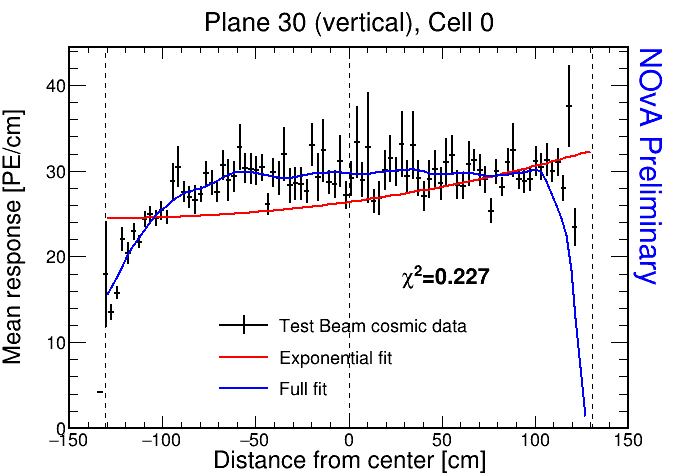
\includegraphics[width=\textwidth]{Plots/TBCalibration/ExampleForBrightFile_fb0_030_000.png}
\end{subfigure}
%\hfill
\begin{subfigure}[b]{0.495\textwidth}
\centering
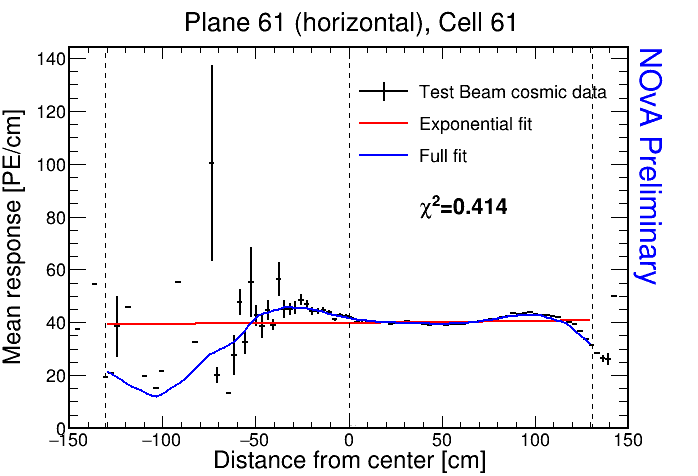
\includegraphics[width=\textwidth]{Plots/TBCalibration/ExampleForBrightFile_fb5_061_061.png}
\end{subfigure}
\caption[Example of failed attenuation fits used for the Test Beam fibre brightness file]{Examples of attenuation fits for two cells that fail the calibration condition, but the fit (blue line) still correctly represents the energy deposition in the centre of that cell (dashed vertical line in the middle).}
\label{fig:FiberBrightnessExamples}
\end{figure}

The final distribution of fibre brightness bins and their corresponding relative brightnesses for the Test Beam detector is shown in Fig.~\ref{fig:NOvAFiberBrightness}.

\subsection{Threshold and Shielding Corrections}
We created the threshold and shielding correction for Test Beam from the new simulation described in Sec.~\ref{sec:DataBasedSimulation}. As can be seen in Fig.~\ref{fig:TBThresholdCorrections}, the correction is almost uniform as a function of both the position within each cell and the cell number. This is the case for all the Test Beam fibre brightness bins and for both views.

The uniformity of the distributions is expected, as the Test Beam detector is much smaller than the \gls{FD}, results of which originated the study of the threshold and the shielding effects. The cell length of $2.6\ \unit{m}$ has only a negligible impact on the energy distribution of cosmic muons or on the threshold saturation. Therefore the threshold and shielding correction for Test Beam is only a normalization factor, except for the cell edges, where there is a large variation in the energy response there anyway due to low number of events. Since we apply the correction prior to the relative calibration, which only cares about the relative differences across the detector, a correction consisting of only a shape-less normalization factor does not have any impact on the calibration results.
 
\begin{figure}[hbtp]
\centering
\begin{subfigure}[t]{\textwidth}
\centering
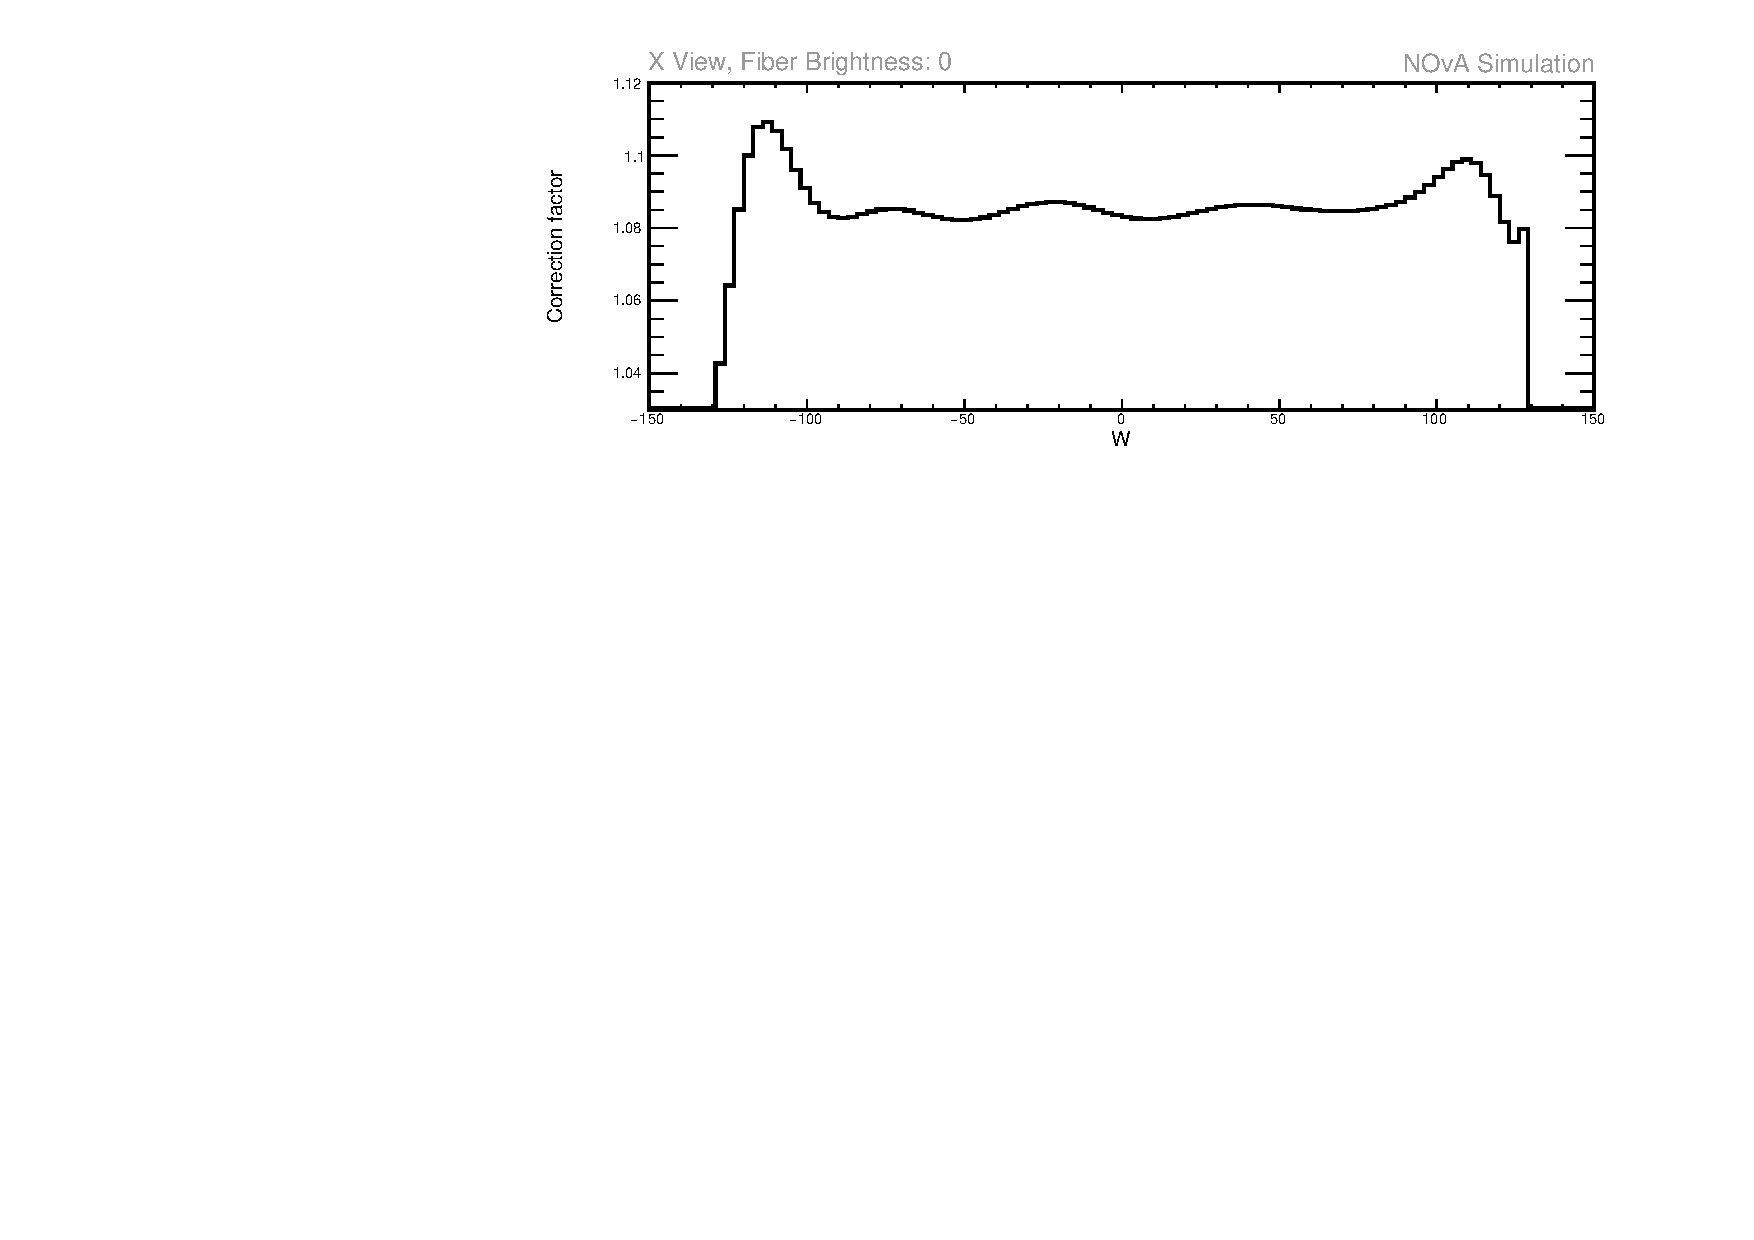
\includegraphics[width=\textwidth]{Plots/TBCalibration/ThresholdCorrectionExample_axview_fb0_P4DataBasedSim.pdf}
\end{subfigure}
\begin{subfigure}[b]{\textwidth}
\centering
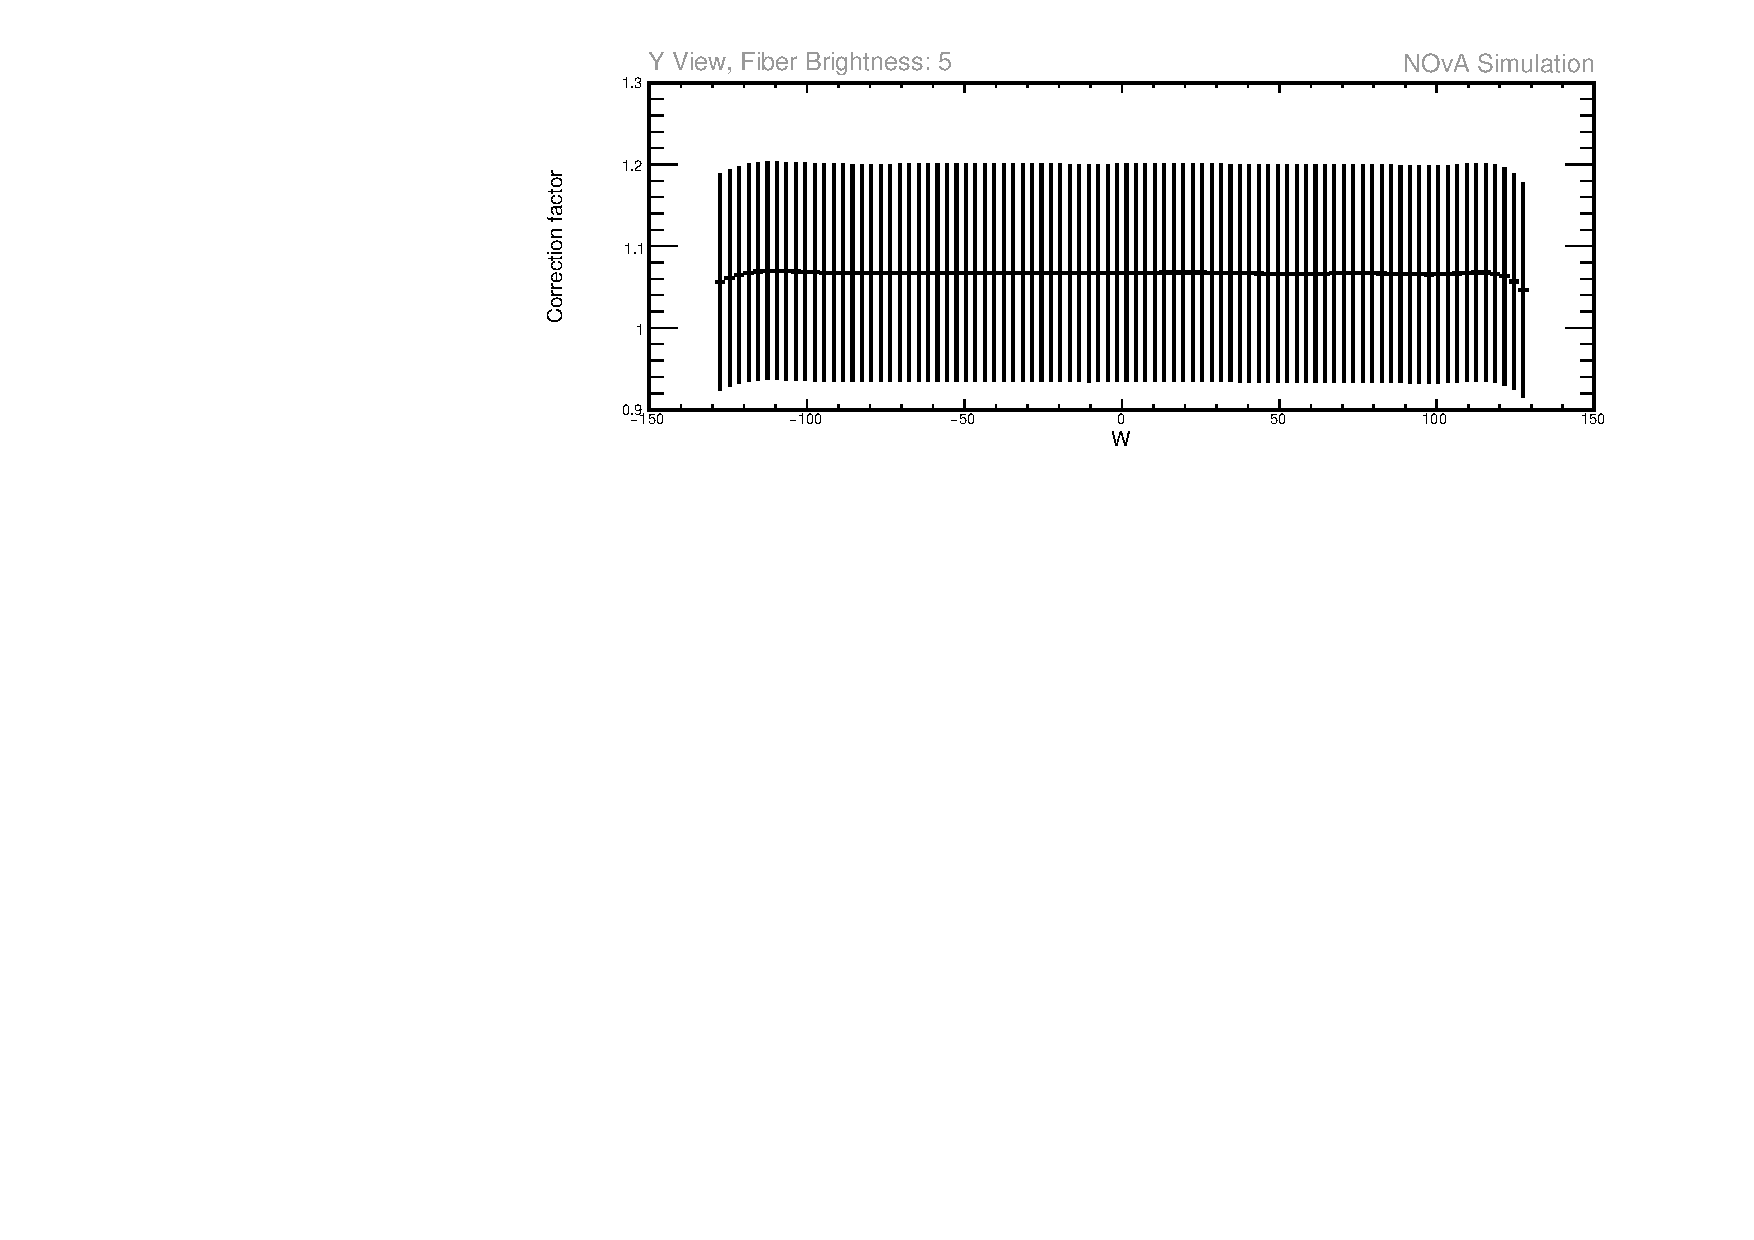
\includegraphics[width=\textwidth]{Plots/TBCalibration/ThresholdCorrectionExample_ayview_fb5_P4DataBasedSim.pdf}
\end{subfigure}
\begin{subfigure}[t]{\textwidth}
\centering
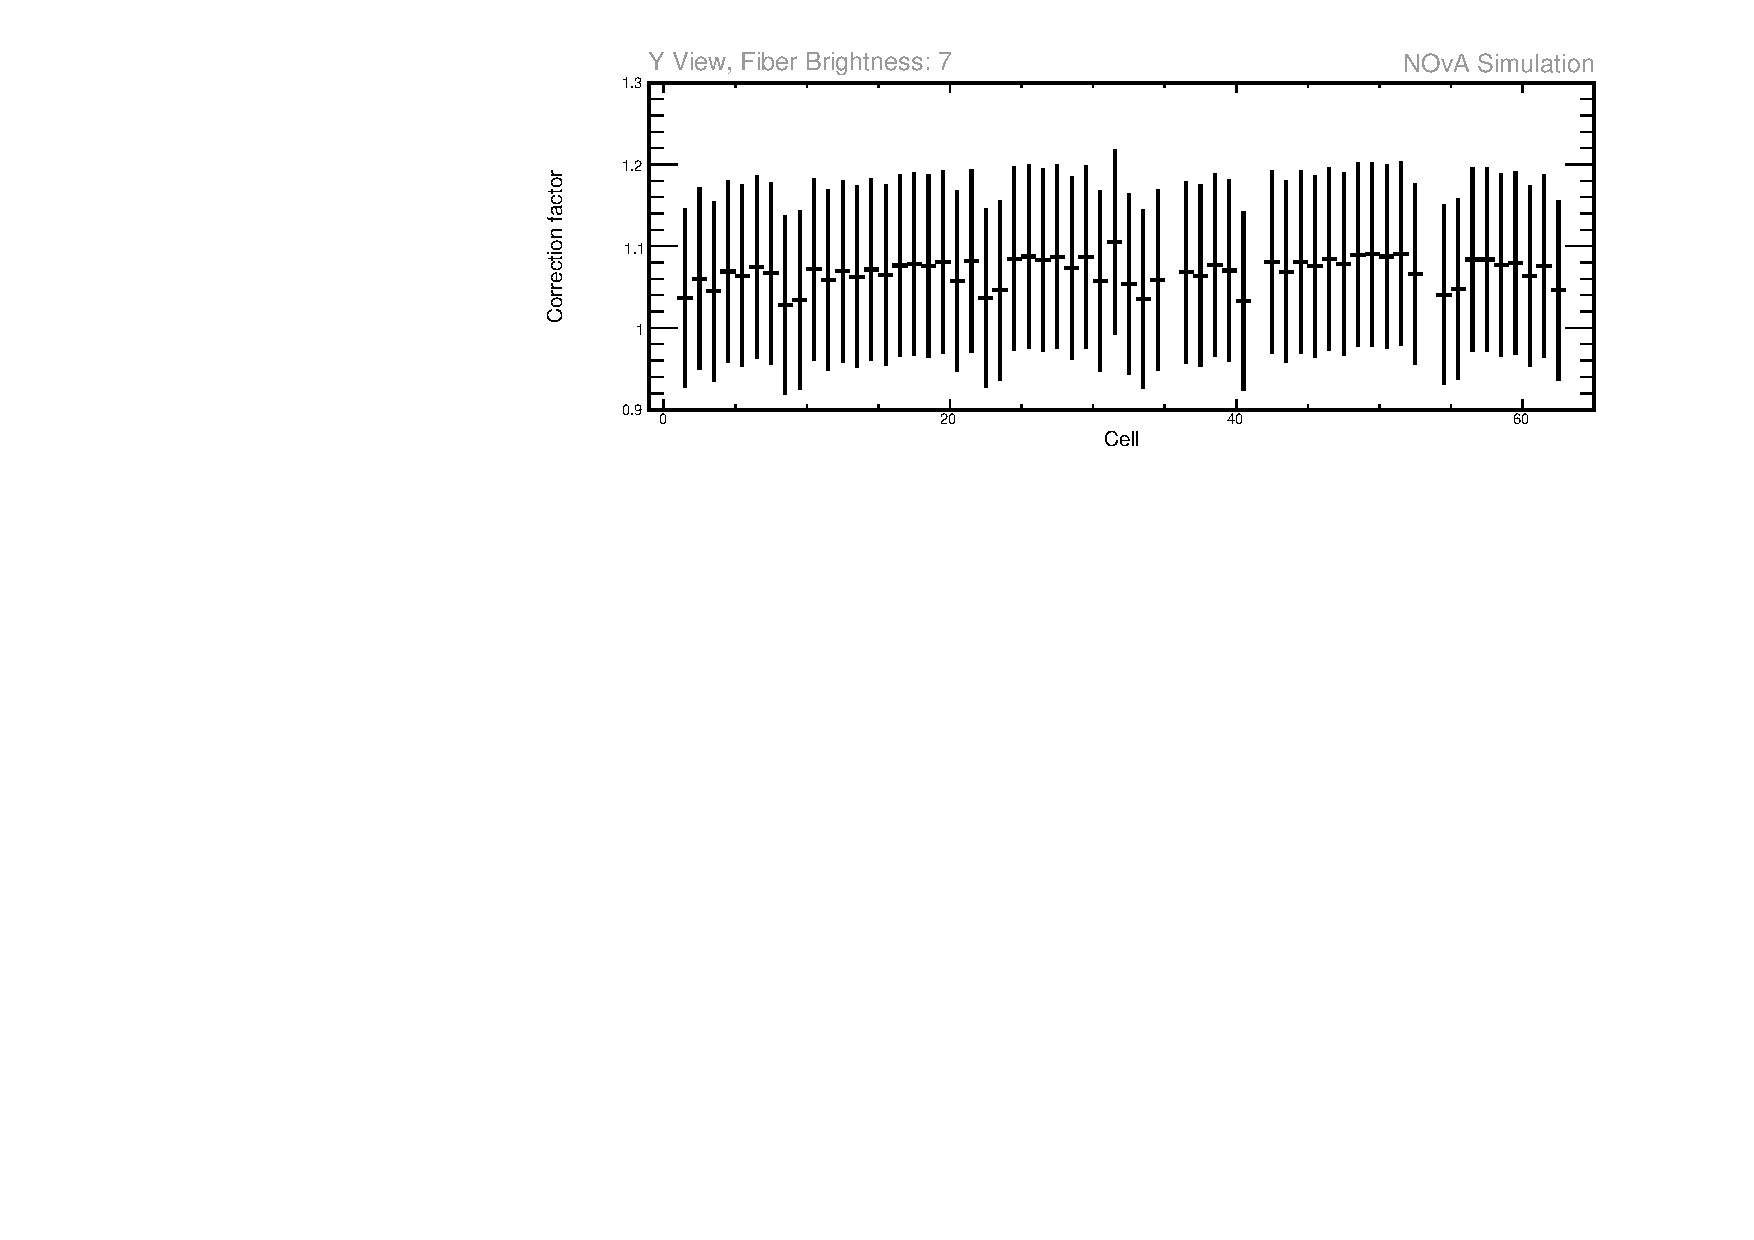
\includegraphics[width=\textwidth]{Plots/TBCalibration/ThresholdCorrectionExample_cyview_fb7_P4DataBasedSim.pdf}
\end{subfigure}
\caption{Examples of threshold and shielding corrections for the Test Beam detector.}
\label{fig:TBThresholdCorrections}
\end{figure}

\subsection{Simulation}\label{sec:SimulationResults}

%Should I talk about the "history" of the simulation of cosmics here, or in the introduction, or not at all?

%We originally used Teresa's calibration MC sample, but after we saw disagreement, we developed a new MC based off of the period 3 data, which we ended up using for both period 2 and period 3. For fibre brightness we are also using the same MC from period 3 data as it represents the detector in its best condition.

We use the data-based simulation described in Sec.~\ref{sec:DataBasedSimulation}. Figure~\ref{fig:CalibhistSim} shows the distribution of the tricell hits from the simulated cosmic muon events selected for calibration. The features on this plot illustrate the distribution of tricell hits in the Test Beam detector in ideal conditions and are present in all the data samples as well. We can clearly see the difference between the number of events in the vertical (even) and the horizontal (odd) planes. This is expected as cosmic muons are generally vertical and a single cosmic track often passes more horizontal planes than vertical planes. We can also see that due to the tricell condition there are no hits in cells 0 and 63, which are on the edge of the detector. The clear horizontal lines are made up by cells (0), 15, 16, 31, 32, 47, 48, (63), or in other words by the first and last cell of each 16 cell-wide extrusion that makes up half of a module (which makes up half of the Test Beam plane). As was mentioned in Sec.~\ref{sec:NOvADetectors}, these cells are $\unit[3]{mm}$ narrower than the rest, which results in fewer hits and lower deposited energy, but consistent deposited energy per path length. Overall, Fig.~\ref{fig:CalibhistSim} shows that the tricell hits are distributed fairly uniformly in the centre of the detector, with the number of hits dropping off towards the front, back and corners of the detector. This is due to the event selection applied to the cosmic tracks to be used in calibration.

\begin{figure}[h]
\centering
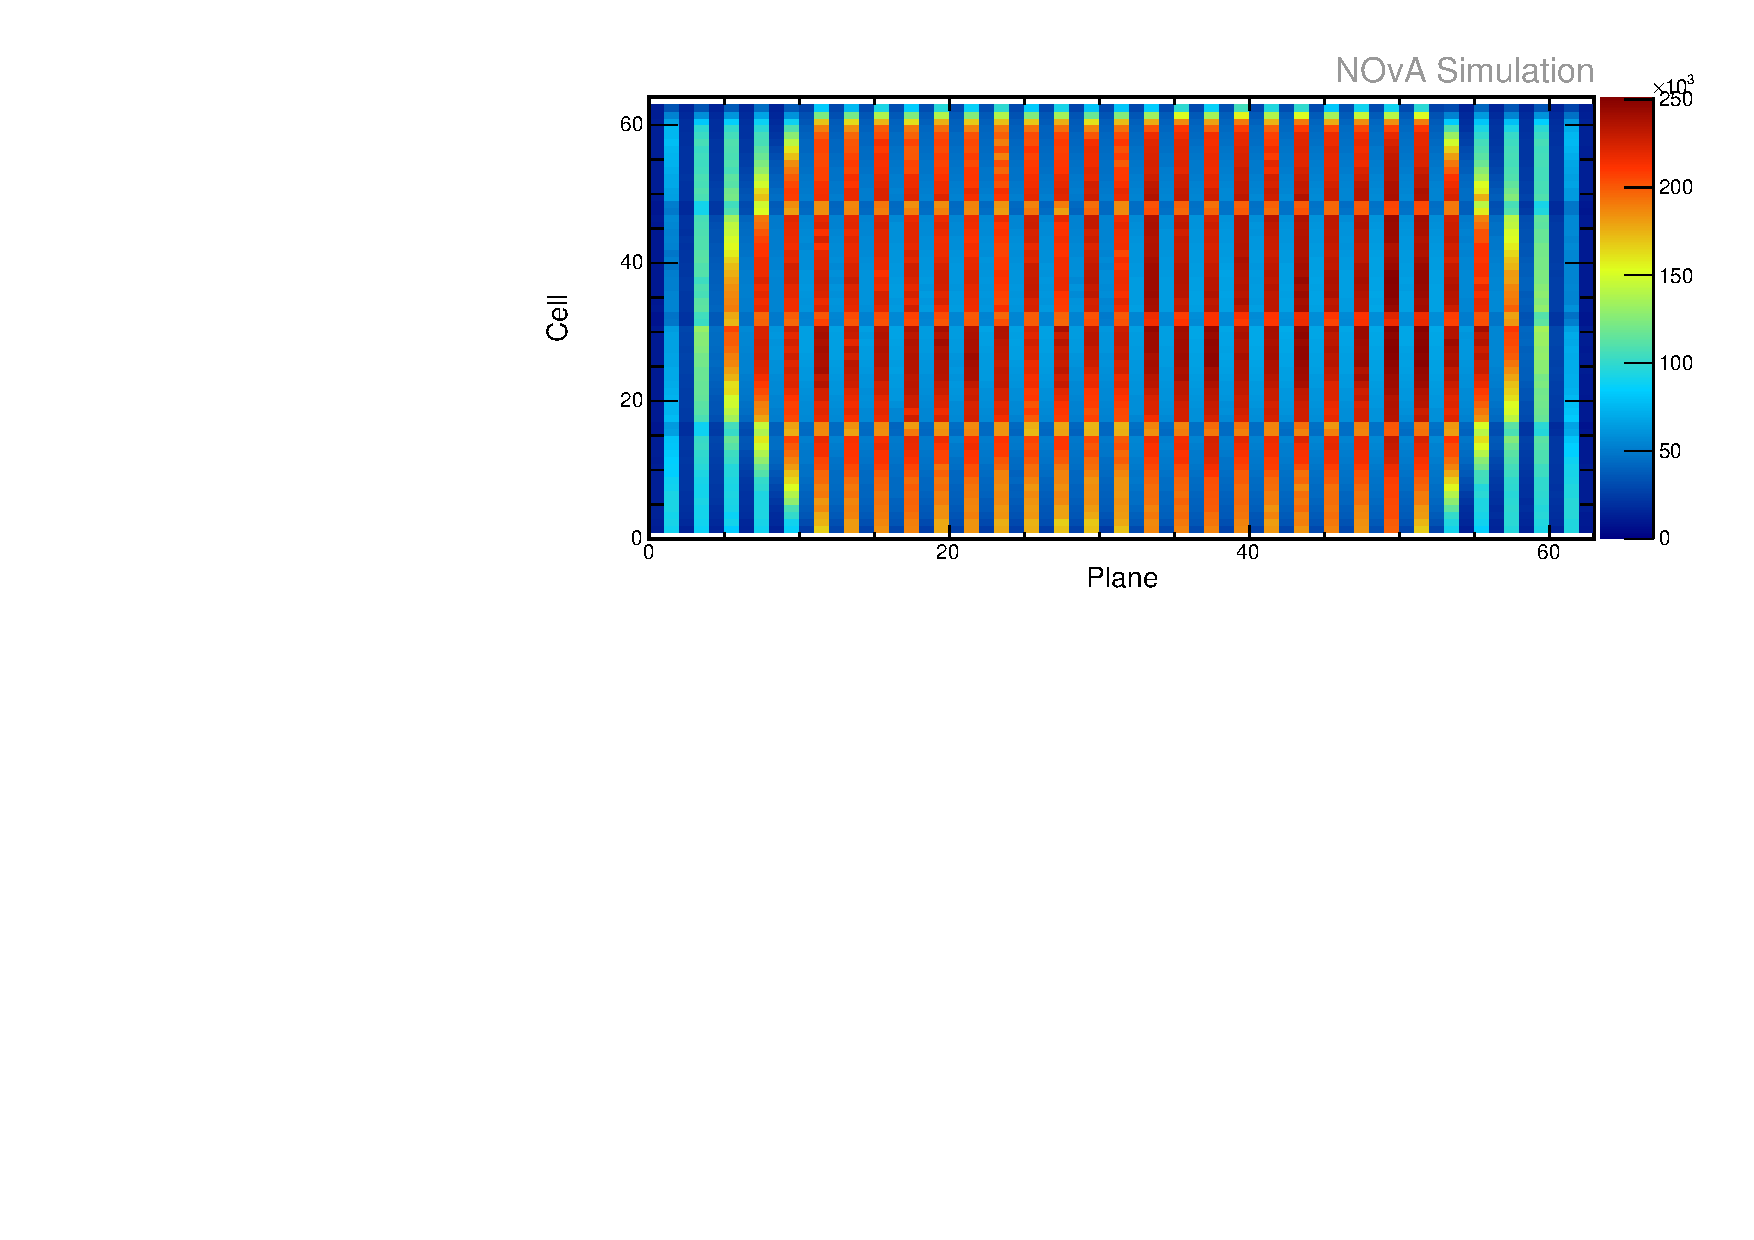
\includegraphics[width=\textwidth]{Plots/TBCalibration/Attenprofs_Simulation_CellPlane.pdf}
\caption[Plane-Cell distribution of hits for the simulation sample]{Distribution of hits used in the calibration for events in the Test Beam simulation calibration sample.}
\label{fig:CalibhistSim}
\end{figure}

The distributions of deposited energy before calibration in units of $\unit{PE/cm}$ are shown in Fig.~\ref{fig:CalibhistWPE_simulation}. We are showing the dependence on the positions within a cell $w$, Cell number and Plane number. These are the distributions that are supposed to be uniform after applying the results of the calibration. We can identify the main features that will need to be corrected for during calibration.

The rise of the energy response along $w$ shown in Fig.~\ref{fig:CalibhistWPE_simulation} is caused by the attenuation of light along the \gls{WLS} fibres. The drop of the response at the edges of the cell is caused by the fibres looping and connecting to the \gls{APD} and the larger uncertainties at the edges of the cell are caused by lower number of hits passing the event selection and the tricell condition.

\begin{figure}[h]
\centering
\begin{subfigure}[b]{0.495\textwidth}
\centering
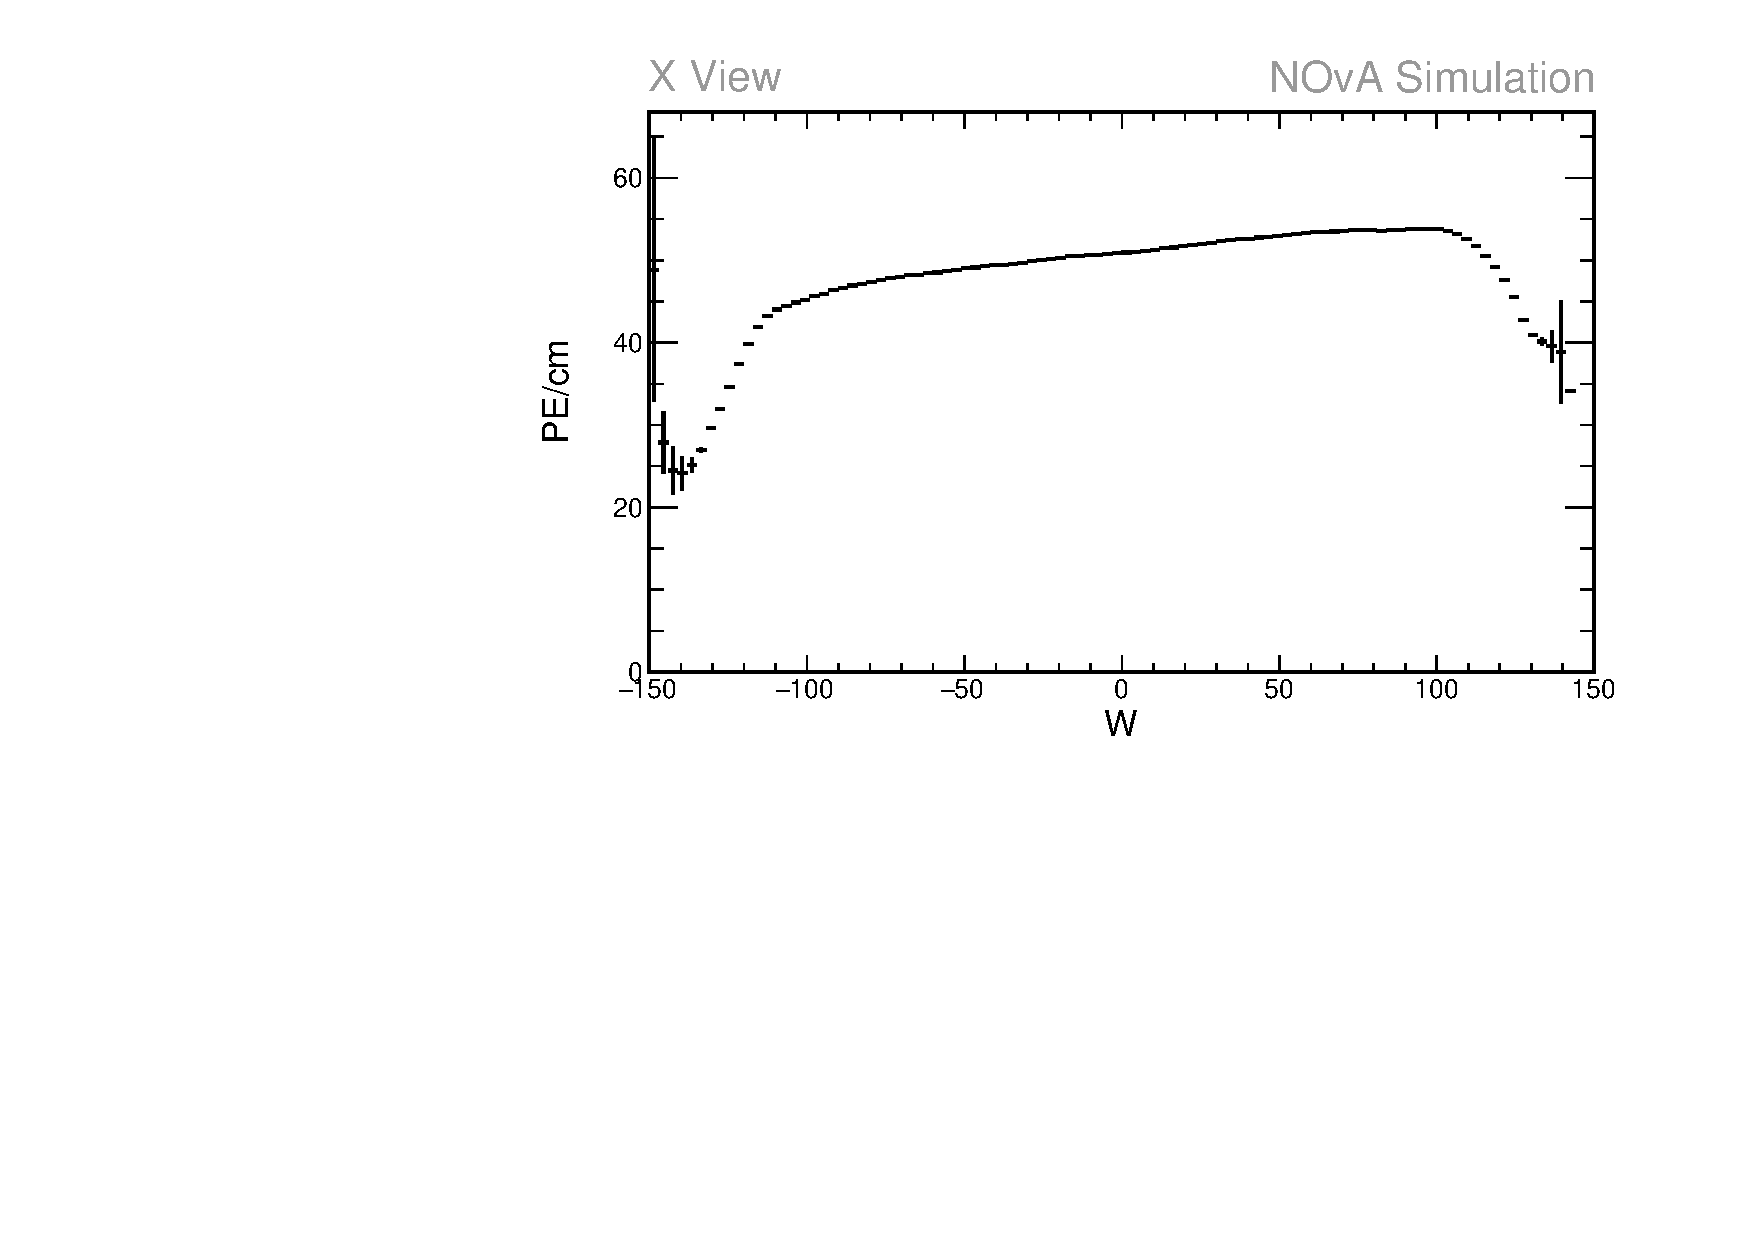
\includegraphics[width=\textwidth]{Plots/TBCalibration/Attenprofs_Simulation_WPE_corr_xy_X_Prof.pdf}
\end{subfigure}
\begin{subfigure}[b]{0.495\textwidth}
\centering
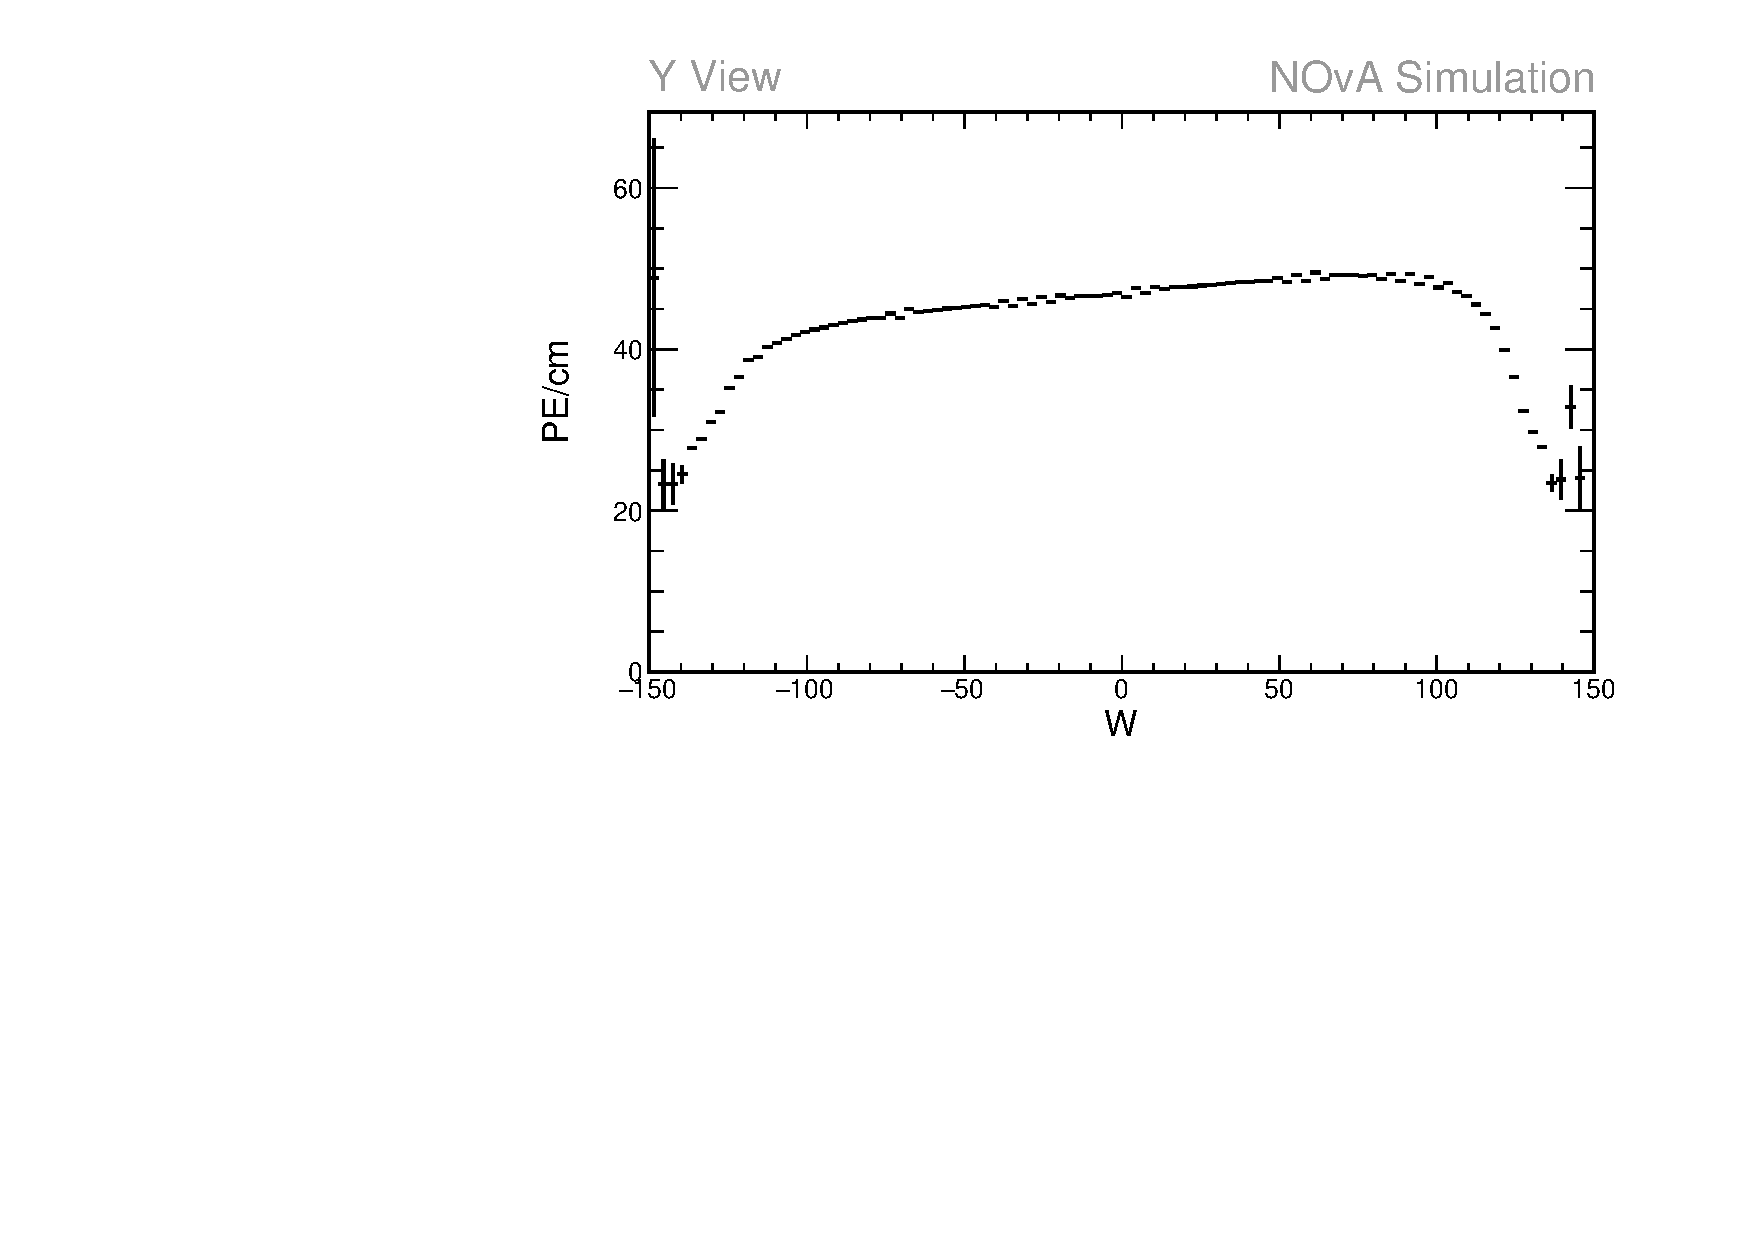
\includegraphics[width=\textwidth]{Plots/TBCalibration/Attenprofs_Simulation_WPE_corr_xy_Y_Prof.pdf}
\end{subfigure}
\caption[Uncorrected energy response along the position within a cell for simulation]{Uncorrected average energy response along the position within a cell ($w$) for simulation. Left side shows distributions for the X view planes and right side for the Y view planes.}
\label{fig:CalibhistWPE_simulation}
\end{figure}

The rise of the response along the cell number shown on the middle plots of Fig.~\ref{fig:CalibhistCellPE_simulation} is due to the varying distance of the cells to the readout. Since the \gls{APD}s are located on a side of each module, the light from the cells on the opposite side has to travel along the \gls{WLS} fibre for the additional width of the module, compared to the cells close to the readout. Light undergoes additional attenuation along these so-called pig tails, causing the difference of the energy response.

We can also see additional drops in the uncorrected energy response for cells 0, 1, 9, 10, 23, 24, 31 and 32 (and the corresponding cells in the second module). These are most likely related to the organization of the \gls{WLS} fibres' connections to the \gls{APD}s. As can be seen in Fig.~\ref{fig:NOvAAPD}, the fibres are connected to the total 32 \gls{APD} pixels in four rows of 8 pixels. Therefore, if one side of each \gls{APD} has a lower response than the rest, this could explain the drop in the energy response for the aforementioned mentioned cells. However, this has not been confirmed yet and the reason for one side of the \gls{APD} having a lower response than the rest is unclear. \note{Also I need to make sure that the pixel organization on the APD is the way I explain it here}

\begin{figure}[h]
\centering
\begin{subfigure}[b]{0.495\textwidth}
\centering
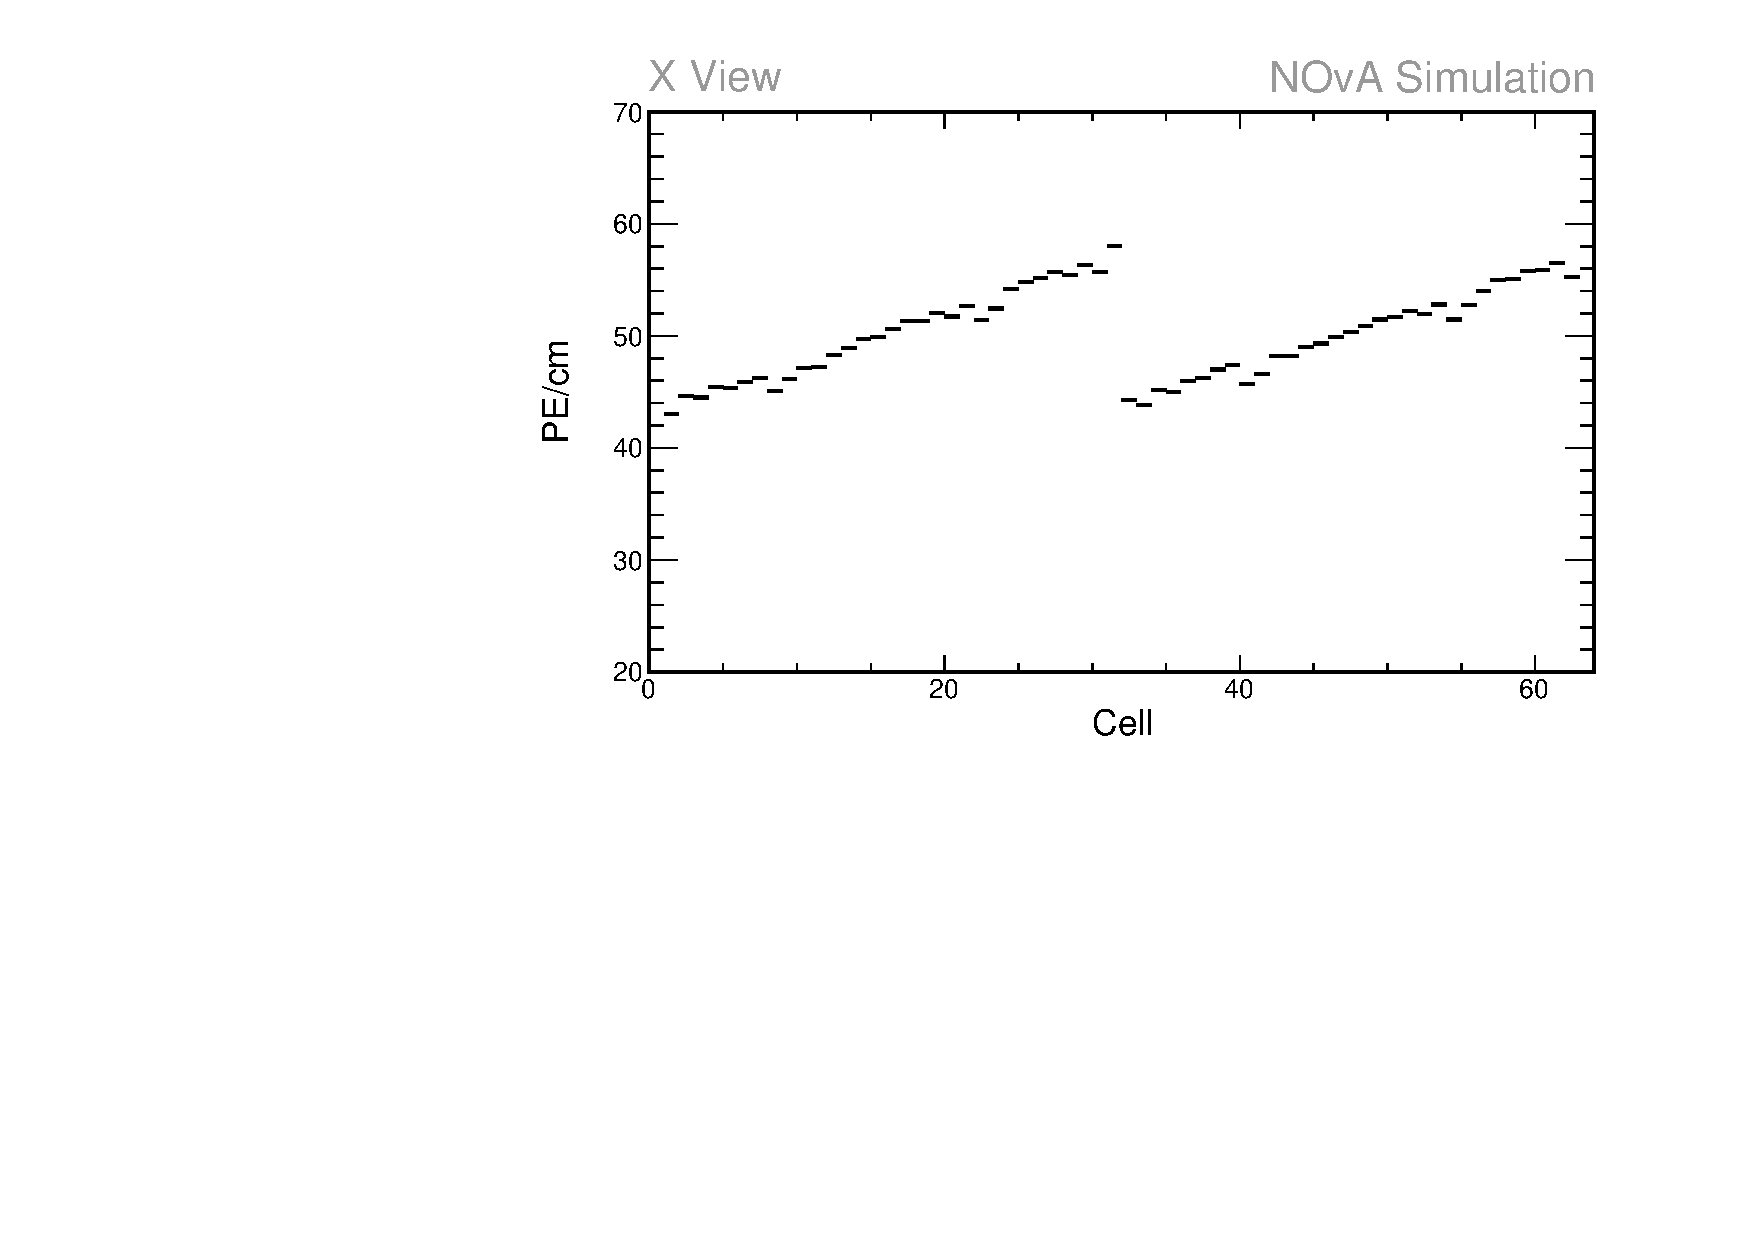
\includegraphics[width=\textwidth]{Plots/TBCalibration/Attenprofs_Simulation_CellPE_X_Prof.pdf}
\end{subfigure}
\begin{subfigure}[b]{0.495\textwidth}
\centering
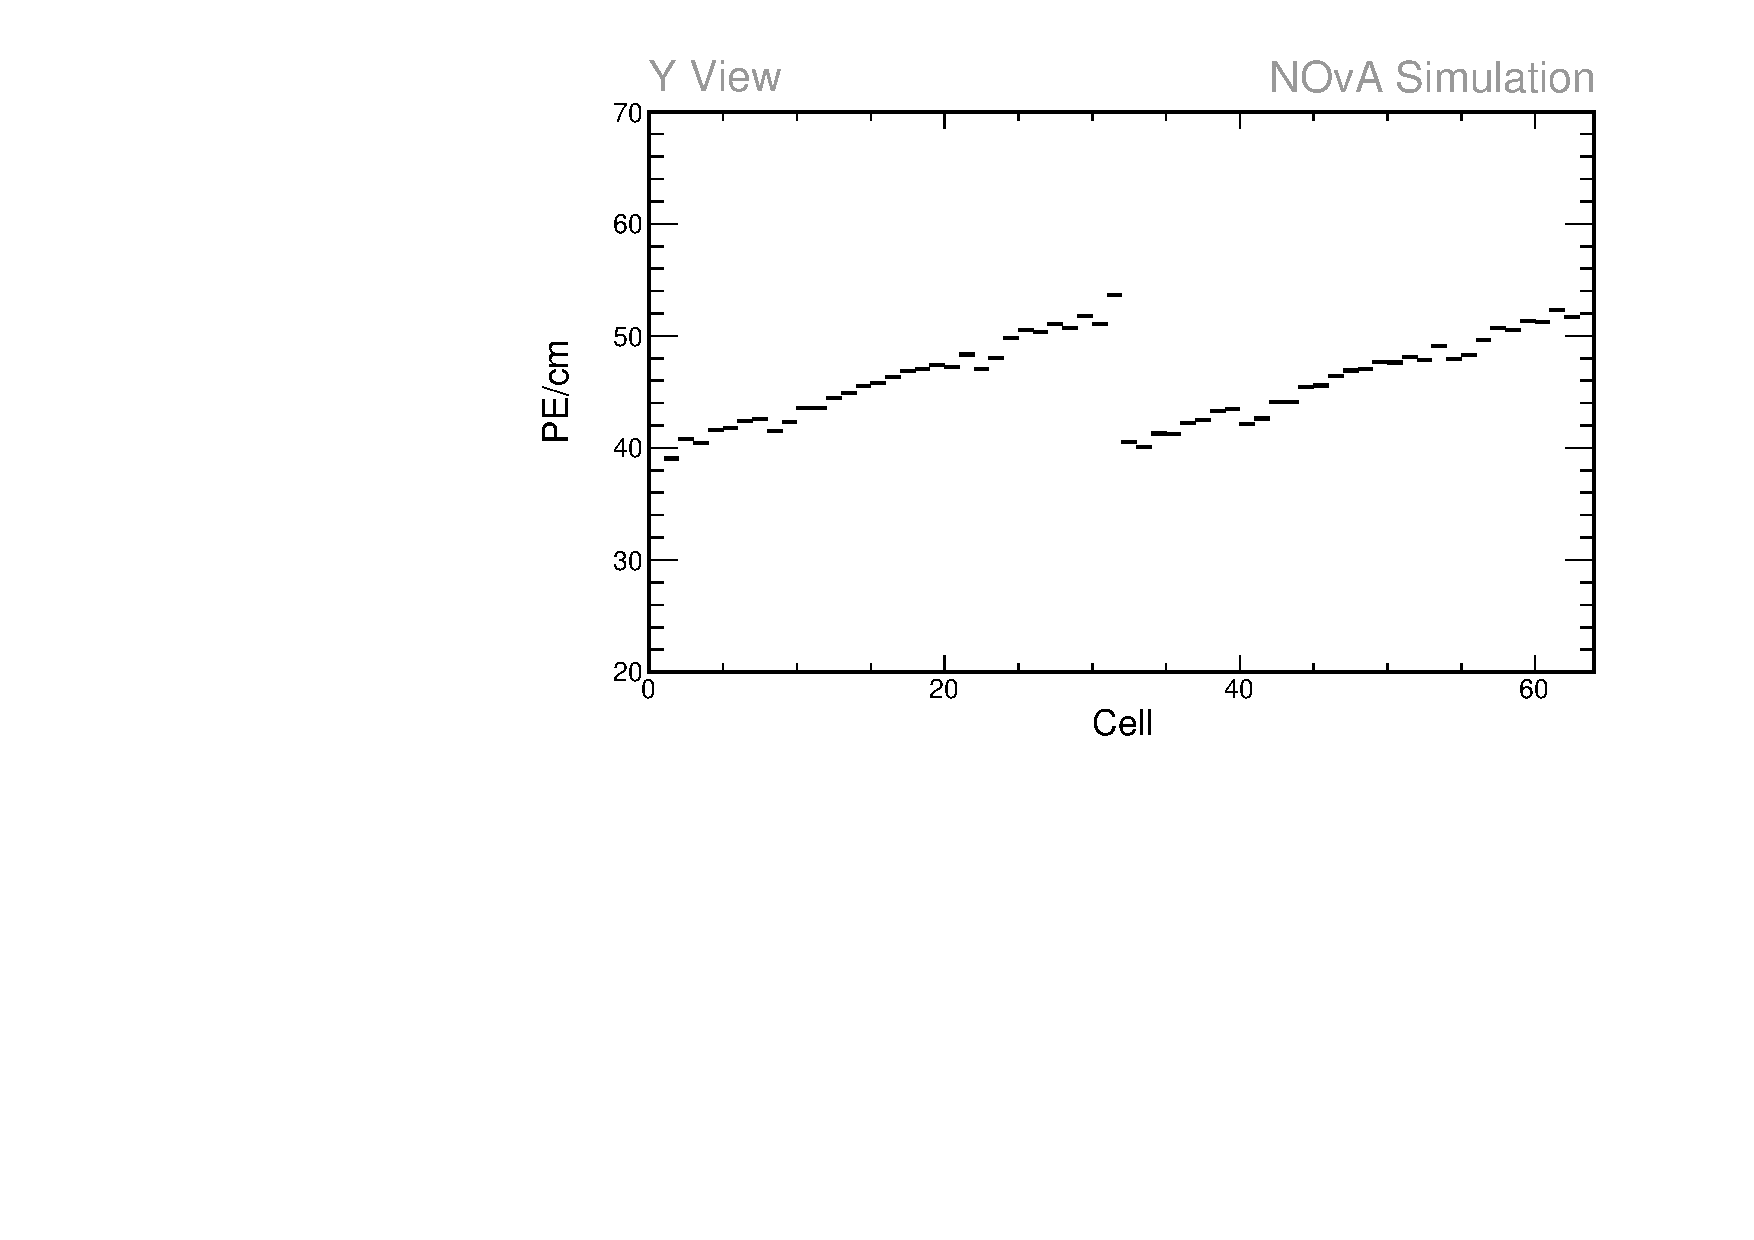
\includegraphics[width=\textwidth]{Plots/TBCalibration/Attenprofs_Simulation_CellPE_Y_Prof.pdf}
\end{subfigure}
\caption{Uncorrected average energy response along cells for simulation.}
\label{fig:CalibhistCellPE_simulation}
\end{figure}

The distribution of the uncorrected response along the planes is shown in Fig.~\ref{fig:CalibhistPlanePE_simulation}. Here we can see large fluctuations in both views, but we can clearly identify the three distinctly different responses corresponding to the various scintillators used, as we described in Sec.\ref{sec:TBExperiment}. Additionally, planes 16, 17, 48 and 49 have a lower response relative to their neighbouring planes due to the different readout electronics used in these planes.

\begin{figure}[h]
\centering
\begin{subfigure}[b]{0.495\textwidth}
\centering
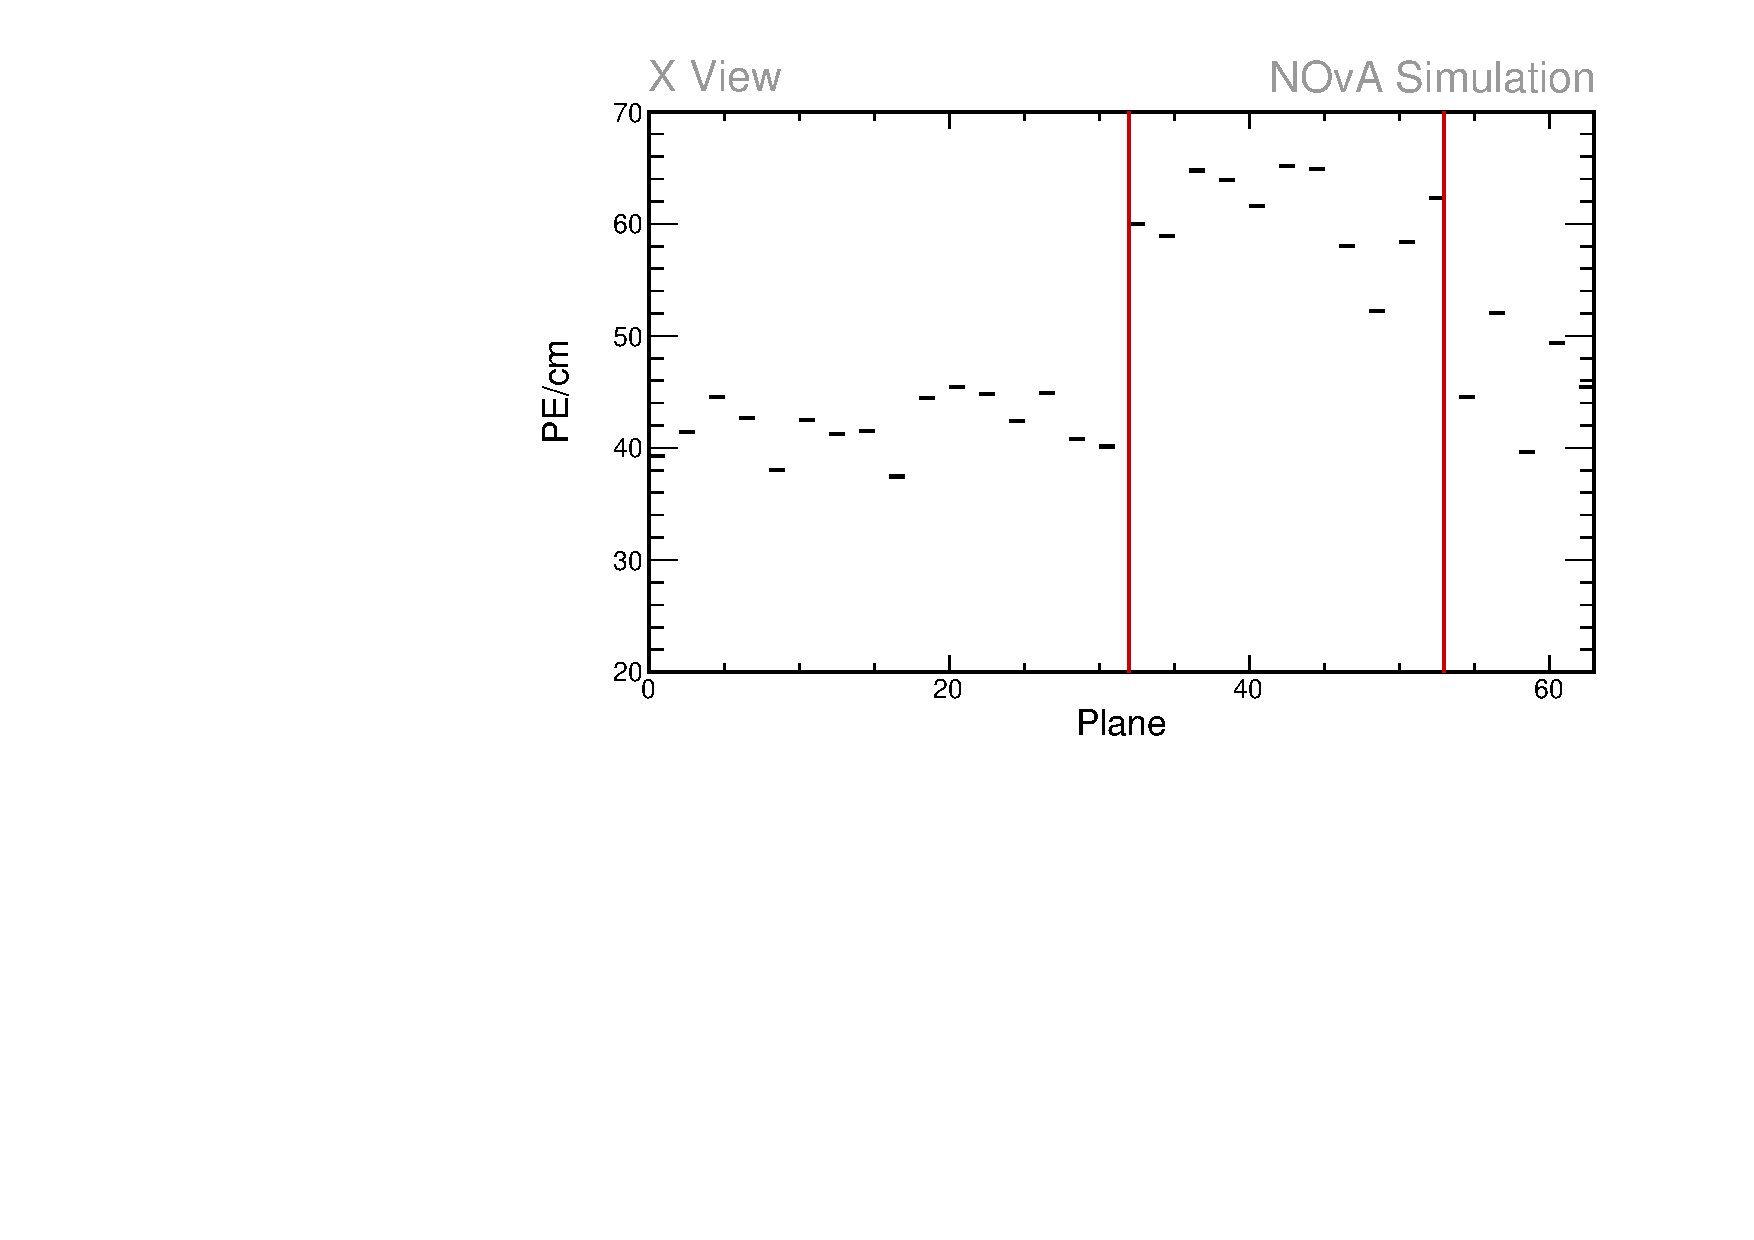
\includegraphics[width=\textwidth]{Plots/TBCalibration/Attenprofs_Simulation_PlanePE_X_Prof.pdf}
\end{subfigure}
\begin{subfigure}[b]{0.495\textwidth}
\centering
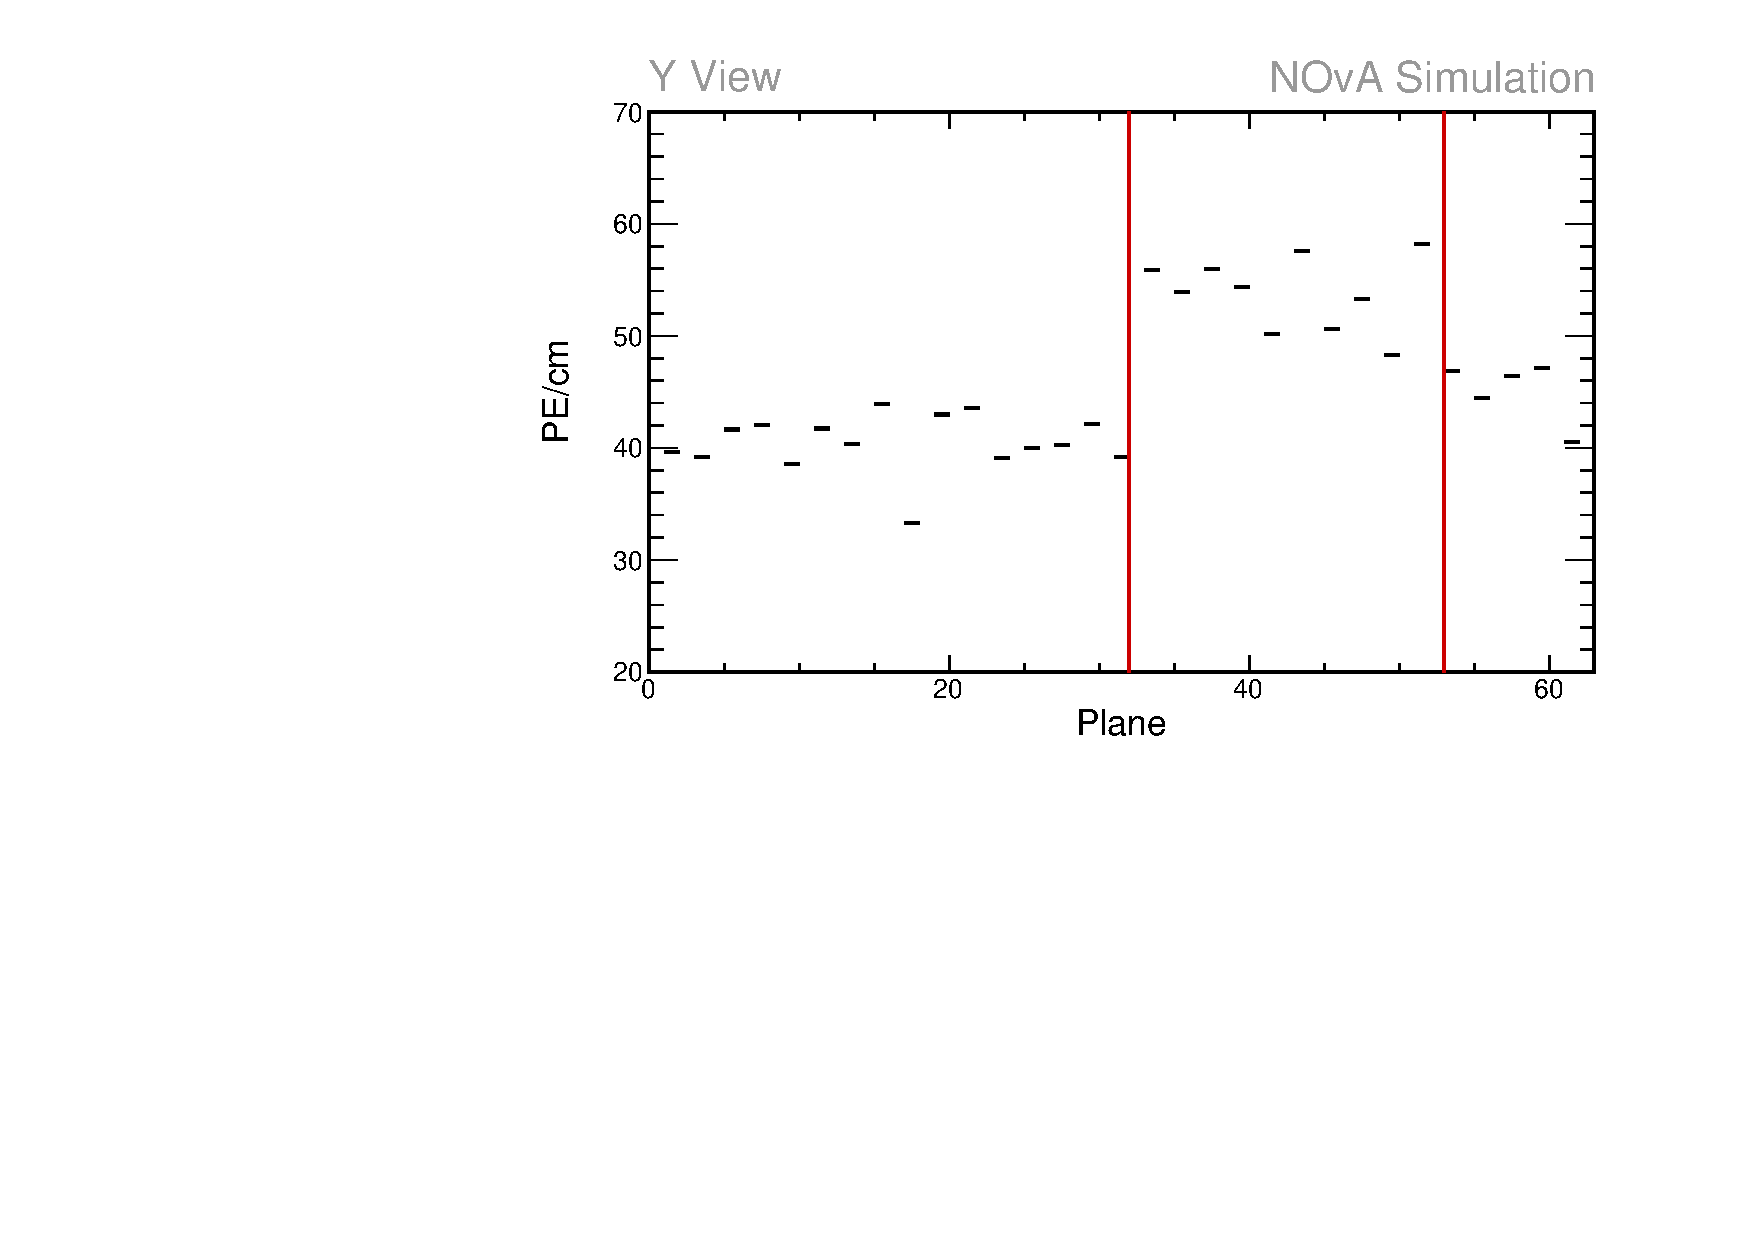
\includegraphics[width=\textwidth]{Plots/TBCalibration/Attenprofs_Simulation_PlanePE_Y_Prof.pdf}
\end{subfigure}
\caption{Uncorrected average energy response along planes for simulation.}
\label{fig:CalibhistPlanePE_simulation}
\end{figure}

\subsubsection*{Simulation Relative Calibration Results}

An overview of the attenuation fit results for simulation are shown in Fig.~\ref{fig:CellCentreResponseSim} as a map of the average fitted response in the centre of each cell. The blank cells show the uncalibrated cells which failed the calibration condition (attenuation fit $\chi^2>0.2$). Most of the uncalibrated cells are on the edges of the detector, which is expected as those have much fewer events that pass the calibration sample selection than the rest. There are a total of 43 uncalibrated cells out of the total 4032 cells, resulting in 1.07\% of the simulated detector uncalibrated.

\begin{figure}[h]
\centering
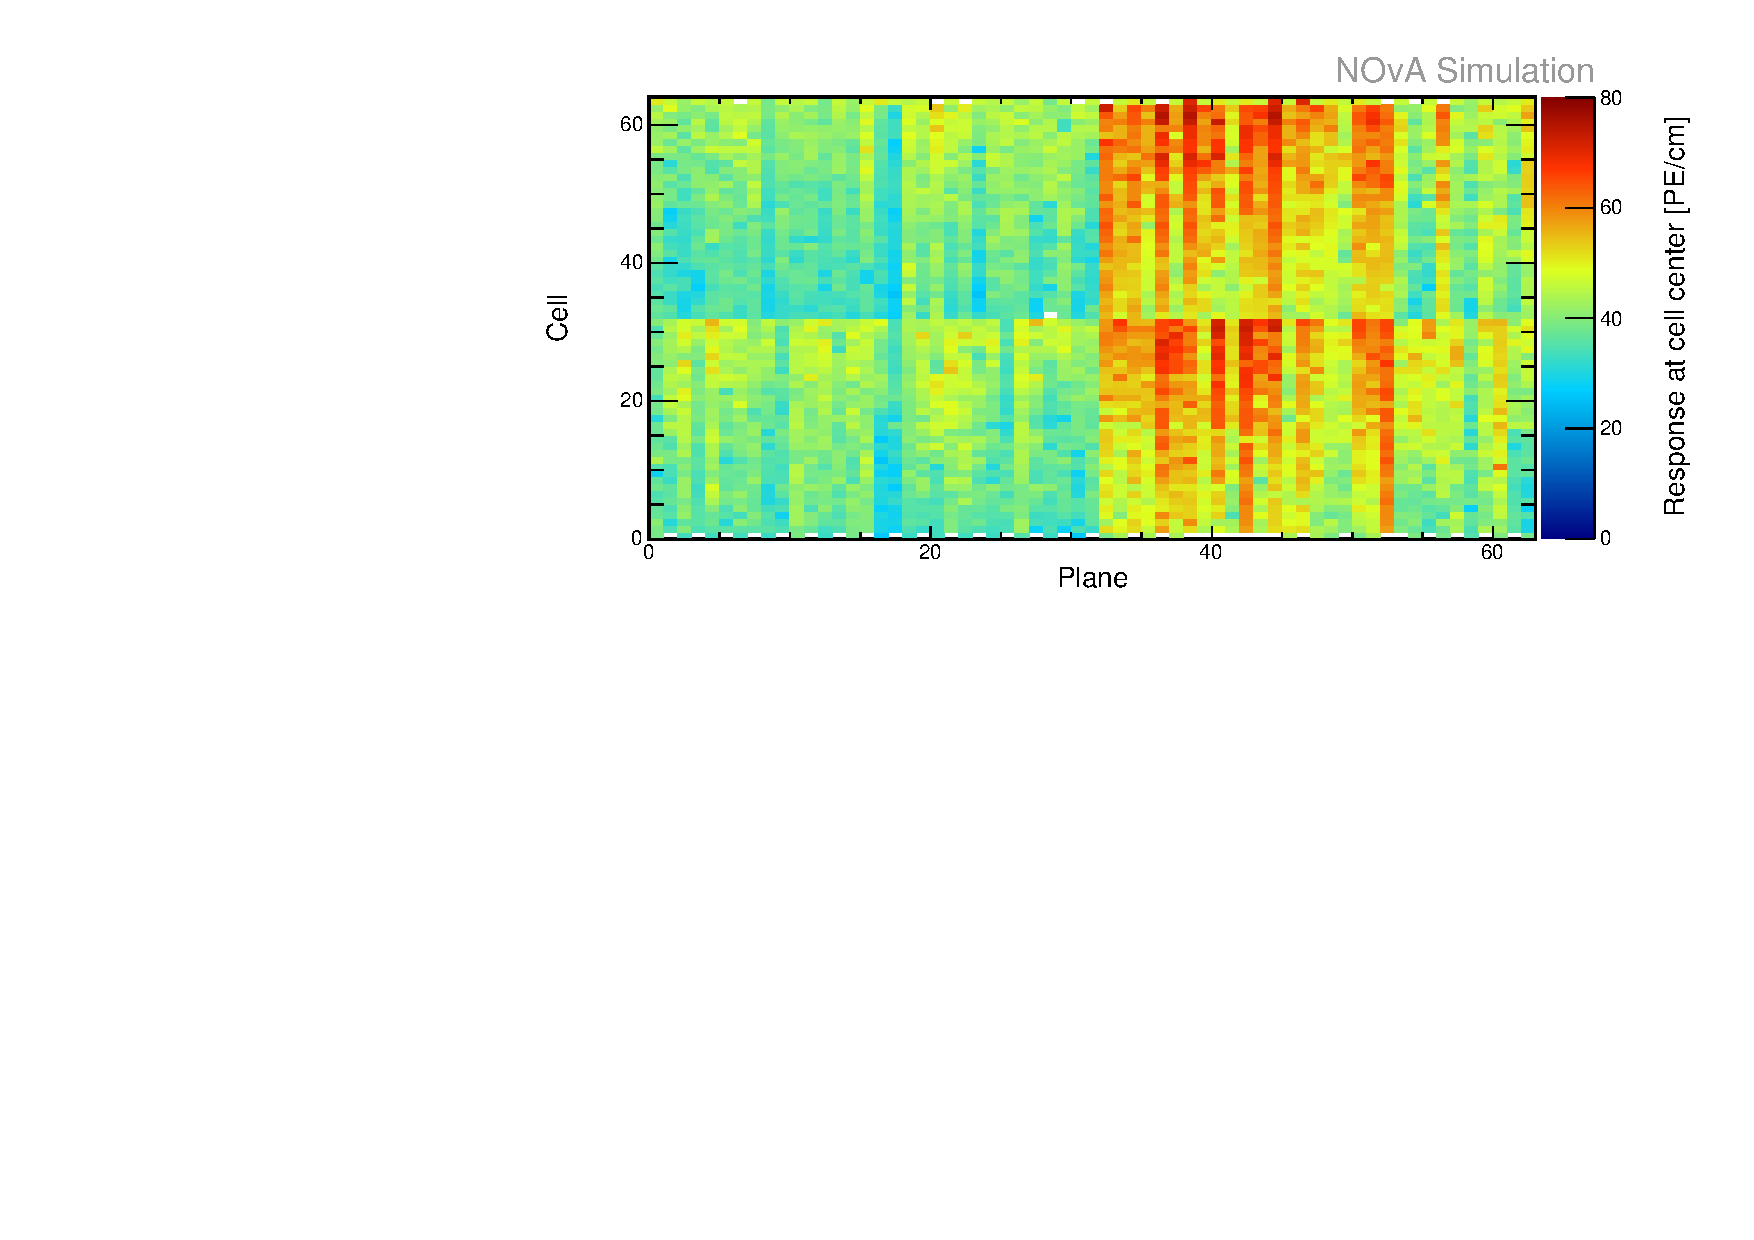
\includegraphics[width=\textwidth]{Plots/TBCalibration/CellResponseAtCentre_Prod4DataBasedSim_Limited_NOvAPlotStyle.pdf}
\caption[Map of fitted response at cell centre for simulation]{Overview of the attenuation fit results for the calibration of the simulated Test Beam detector. Each cell represents the result of the attenuation fit of the energy response in the centre of that cell. The blank cells are uncalibrated as the attenuation fit did not satisfy the calibration condition.}
\label{fig:CellCentreResponseSim}
\end{figure}

Examples of the standard detector response and of the response for cells on the edge of the detector are shown on the top left plot and on the two bottom plots of Fig.~\ref{fig:AttenfitResultsSimulation} respectively. Here the red line shows the initial exponential fit and the blue line the final attenuation fit after the \gls{LOWESS} correction, as described in Sec.~\ref{sec:NOvACalibration}. The cells on the edge of the detector failed the calibration conditions due to the low number of entries causing large fluctuation in the mean response.

There is only one cell in the middle of the detector that is left uncalibrated. This is the cell 32 in a vertical plane in the brightness bin 5, shown on the top right of Fig.~\ref{fig:AttenfitResultsSimulation}, with $\chi^2=0.227$. It seems the reason this cell has a $\chi^2>0.2$ and therefore failed the calibration condition is the unusually high response with a large uncertainty in the right-most bin. It is unclear why this bin has such an elevated mean response, but since this only causes an issue for a single cell, we decided to ignore it.

\begin{figure}[h]
  \begin{subfigure}{0.495\textwidth}
    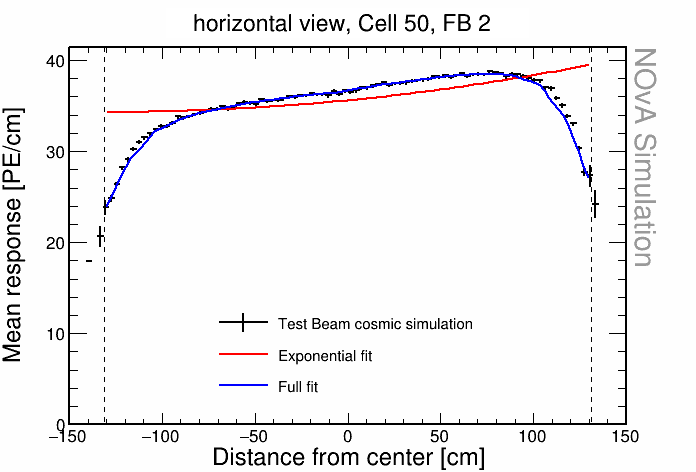
\includegraphics[width=\linewidth]{Plots/RelativeCalibrationResults/sim_fb2_001_050.png}
  \end{subfigure}
  \begin{subfigure}{0.495\textwidth}
    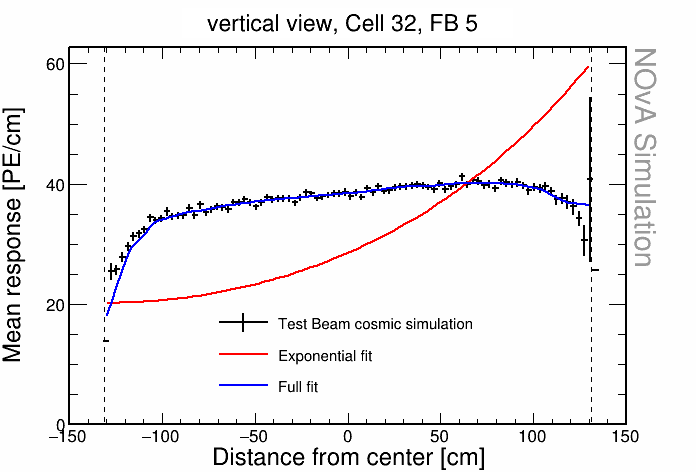
\includegraphics[width=\linewidth]{Plots/RelativeCalibrationResults/sim_fb5_000_032.png}
  \end{subfigure}
  \begin{subfigure}{0.495\textwidth}
    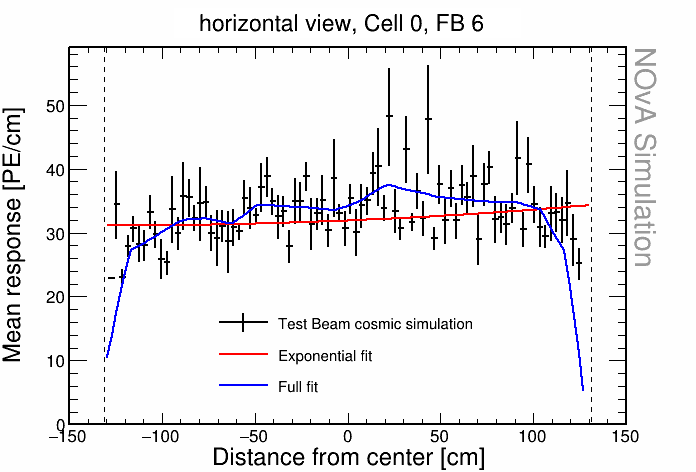
\includegraphics[width=\linewidth]{Plots/RelativeCalibrationResults/sim_fb6_001_000.png}
  \end{subfigure}
  \begin{subfigure}{0.495\textwidth}
    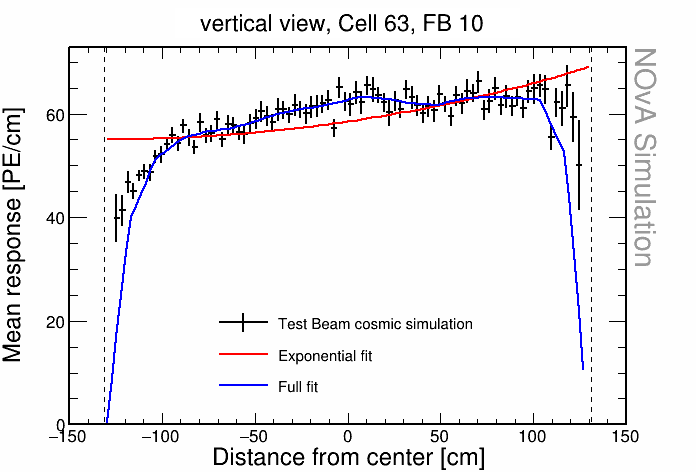
\includegraphics[width=\linewidth]{Plots/RelativeCalibrationResults/sim_fb10_000_063.png}
  \end{subfigure}
  \caption[Example attenuation fits for simulation]{Attenuation fits for a selection of cells in the Test Beam calibration simulation. Top left is an example of a successful attenuation fit, top right is a failed fit due to statistical fluctuation in the last bin and the bottom plots show failed fits for cells on the edges of the detector.}
  \label{fig:AttenfitResultsSimulation}
\end{figure}

\FloatBarrier
\subsection{Period 2 Data}
The issue with underfilled cells described in Sec.~\ref{sec:TBExperiment} was present throughout the period 2 data taking. This can be clearly seen in Fig.~\ref{fig:Calibhist_period2}, represented by the empty cells 31 and 63 in the horizontal planes, which were marked as bad channels and therefore ignored during production of calibration samples. This also affects the neighbouring cells to the underfilled cells, which have fewer events due to the tricell condition (see Sec.~\ref{sec:NOvACalibration}).

\begin{figure}[h]
\centering
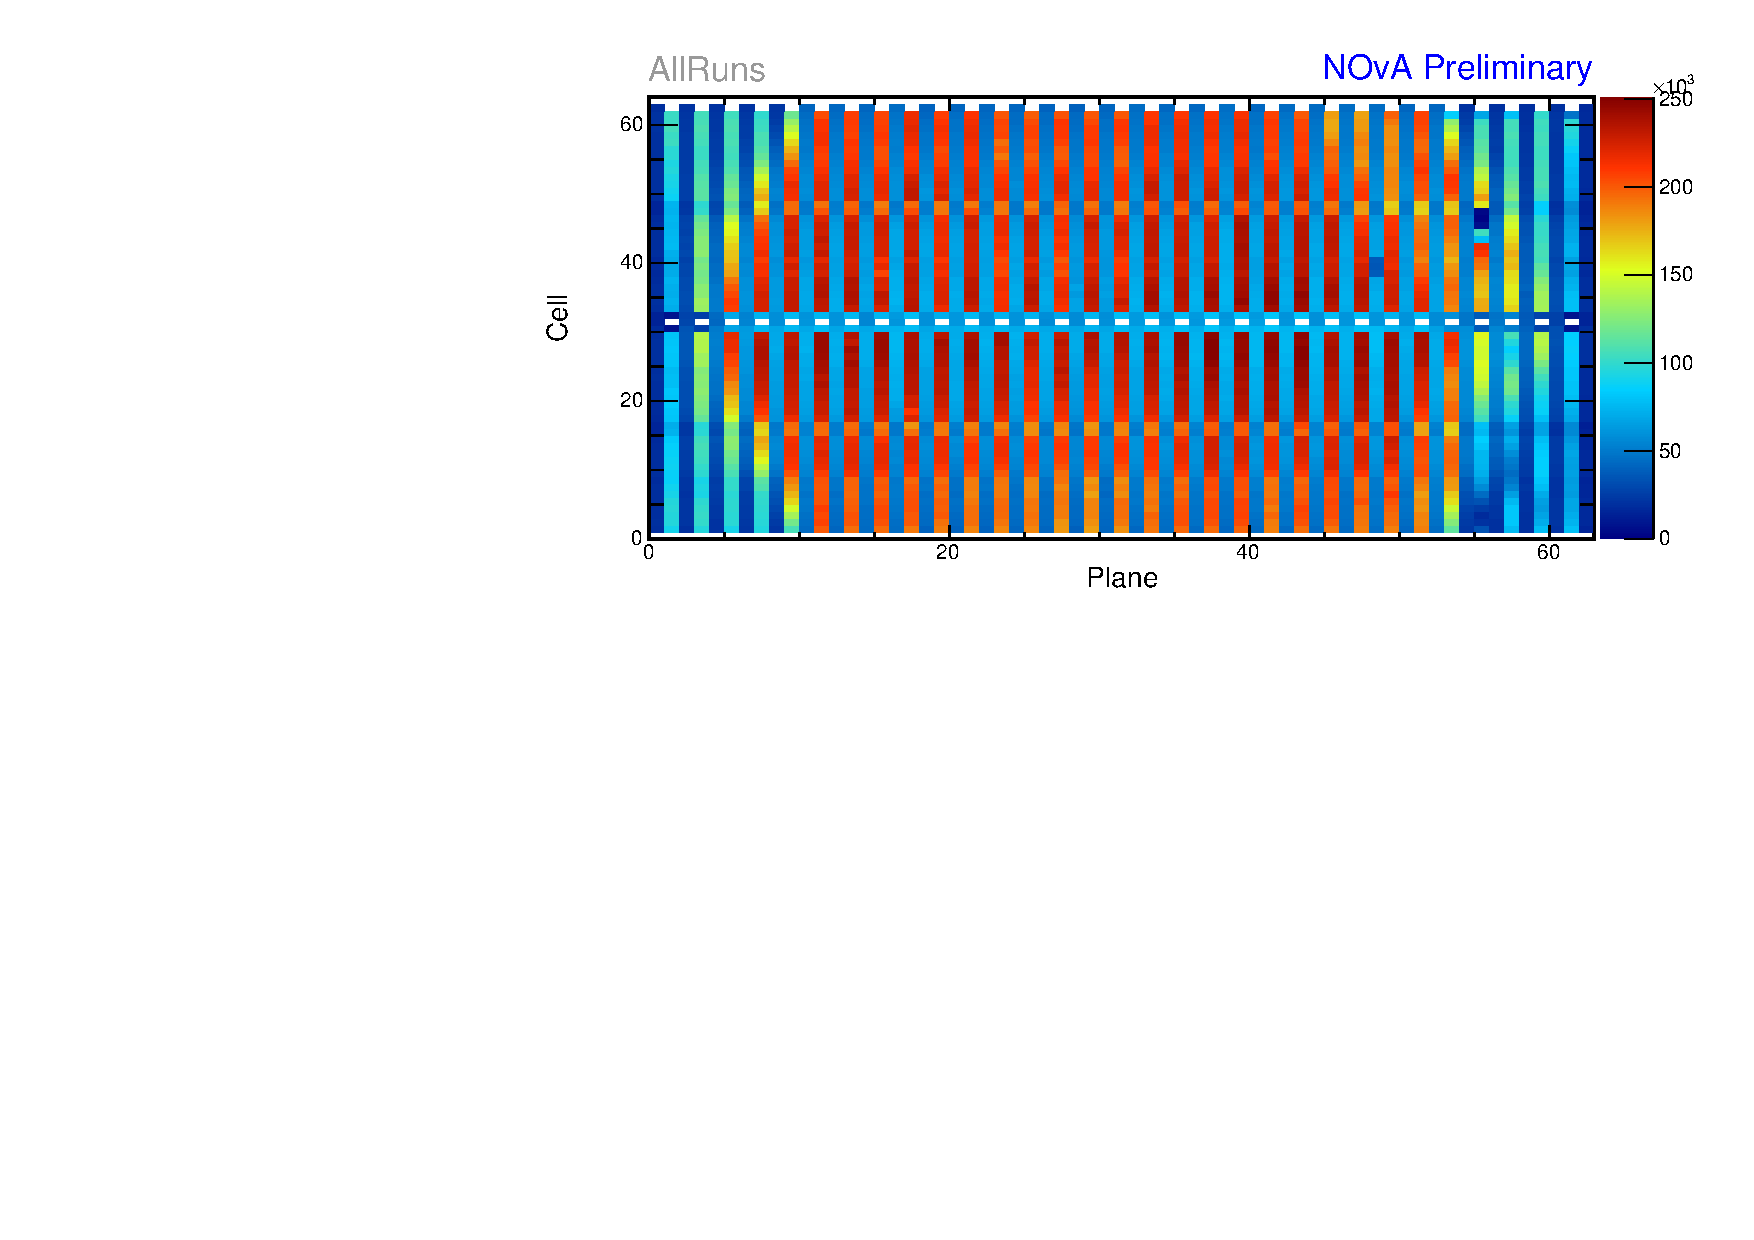
\includegraphics[width=\textwidth]{Plots/TBCalibration/Attenprofs_P2Data_CellPlane_AllRuns.pdf}
\caption[Plane-Cell distribution of hits for the period 2 data sample]{Distribution of events in the period 2 Test Beam data calibration sample.}
\label{fig:Calibhist_period2}
\end{figure}

We can also see three noticeably darker spots than their neighbours. Specifically in plane 48 cells 38-40 and in plane 55 cells 2-4 and 45-47. These are all three cell wide, so it is likely that the issue is only in the middle cells and their immediate neighbours are affected due to the tricell condition. The three affected cells had most likely dead channels for some portion of period 2, with cell 46 in plane 55 being dead the longest. One possible explanation proposed for dead channels in plane 55 is that it is due to switched cables from the readout to the \gls{DAQ} \cite{NOvA-doc-49674}, which is manifested as fewer total number of events in those cells. However, this wouldn't explain the dead channel in cell 39 of plane 48, which was caused by a different issue.

Officially, period 2 is divided into 6 epochs labelled by letters, 2a - 2f, based on the specific running conditions. The epochs mostly differ in the use of various FEB firmwares or trigger studies. We compare the energy deposition in various epochs in Fig.~\ref{fig:CalibhistWPE_period2},\ref{fig:CalibhistCellPE_period2} and \ref{fig:CalibhistPlanePE_period2}. As can be seen, the difference between the energy response across the individual epochs is fairly small and only in normalization. There's also no clear trend of energy response falling or raising with time. The largest outliers seem to be epochs 2a and 2d. Since each individual epoch would not have enough statistics for a successful attenuation fit, we decided to calibrate the entire period 2 together, without splitting it into any smaller samples.

\begin{figure}[h]
\centering
\begin{subfigure}[b]{0.495\textwidth}
\centering
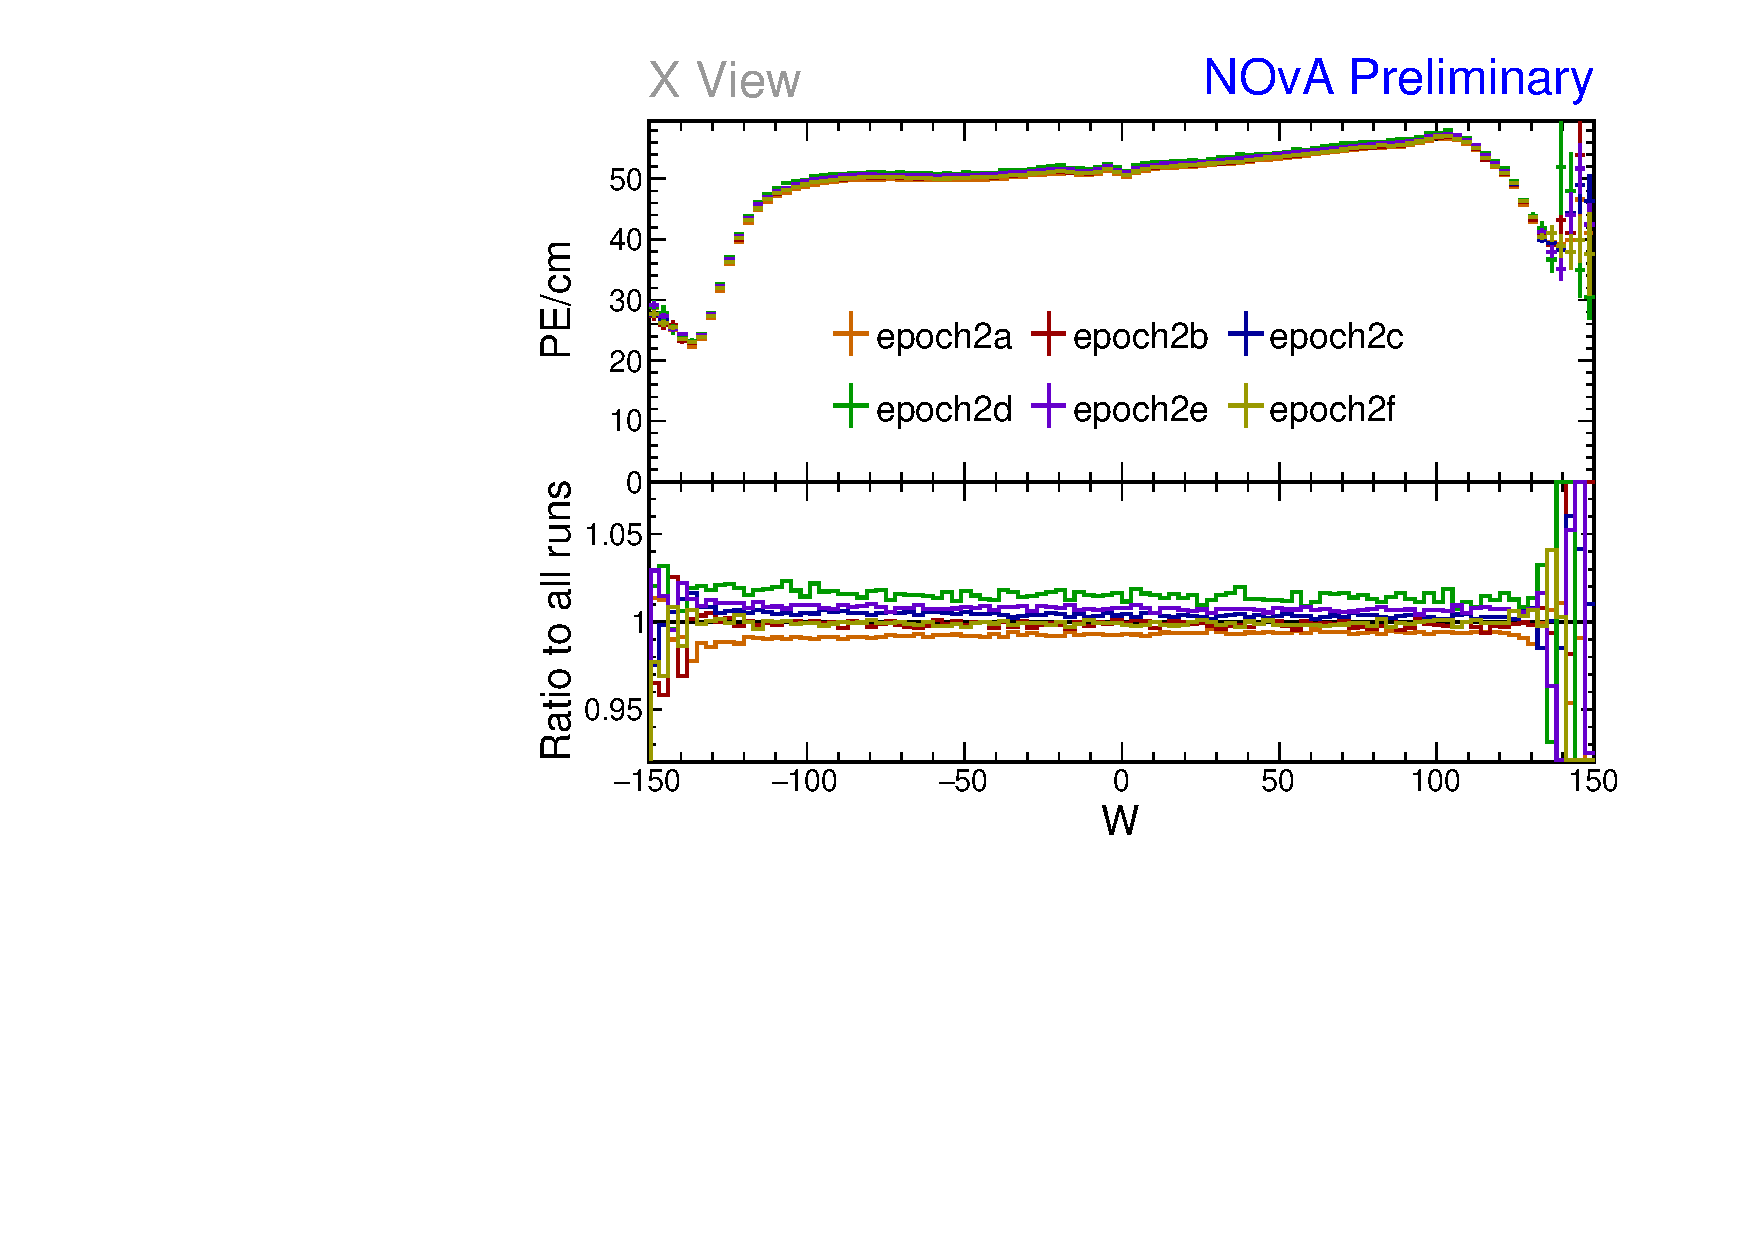
\includegraphics[width=\textwidth]{Plots/TBCalibration/Attenprofs_P2Data_WPE_corr_xy_X_Combined.pdf}
\end{subfigure}
\begin{subfigure}[b]{0.495\textwidth}
\centering
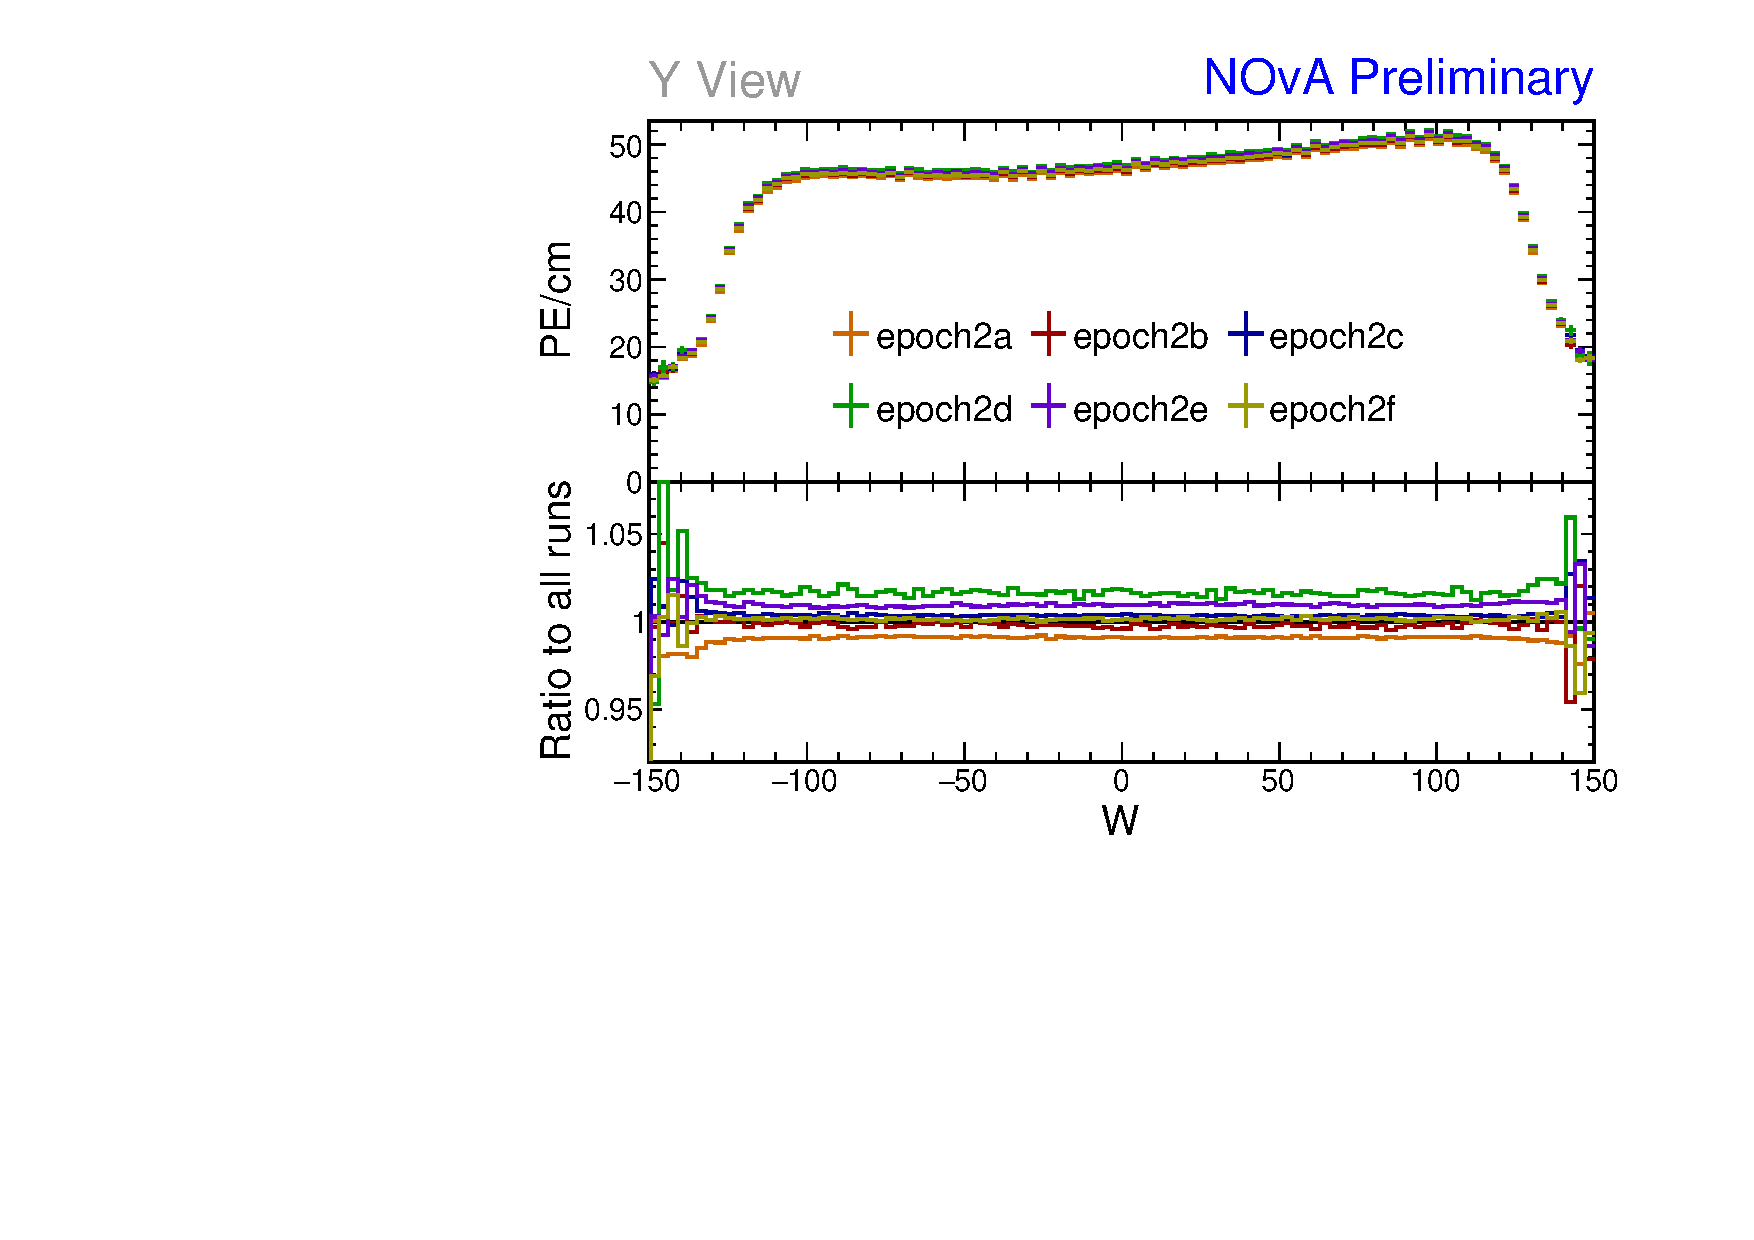
\includegraphics[width=\textwidth]{Plots/TBCalibration/Attenprofs_P2Data_WPE_corr_xy_Y_Combined.pdf}
\end{subfigure}
\caption[Uncorrected energy response along the position within a cell for period 2 data]{Uncorrected average energy response along the position within a cell (w) for epochs in period 2. It is clear that there is no significant difference between the various epochs.}
\label{fig:CalibhistWPE_period2}
\end{figure}

\begin{figure}[h]
\centering
\begin{subfigure}[b]{0.495\textwidth}
\centering
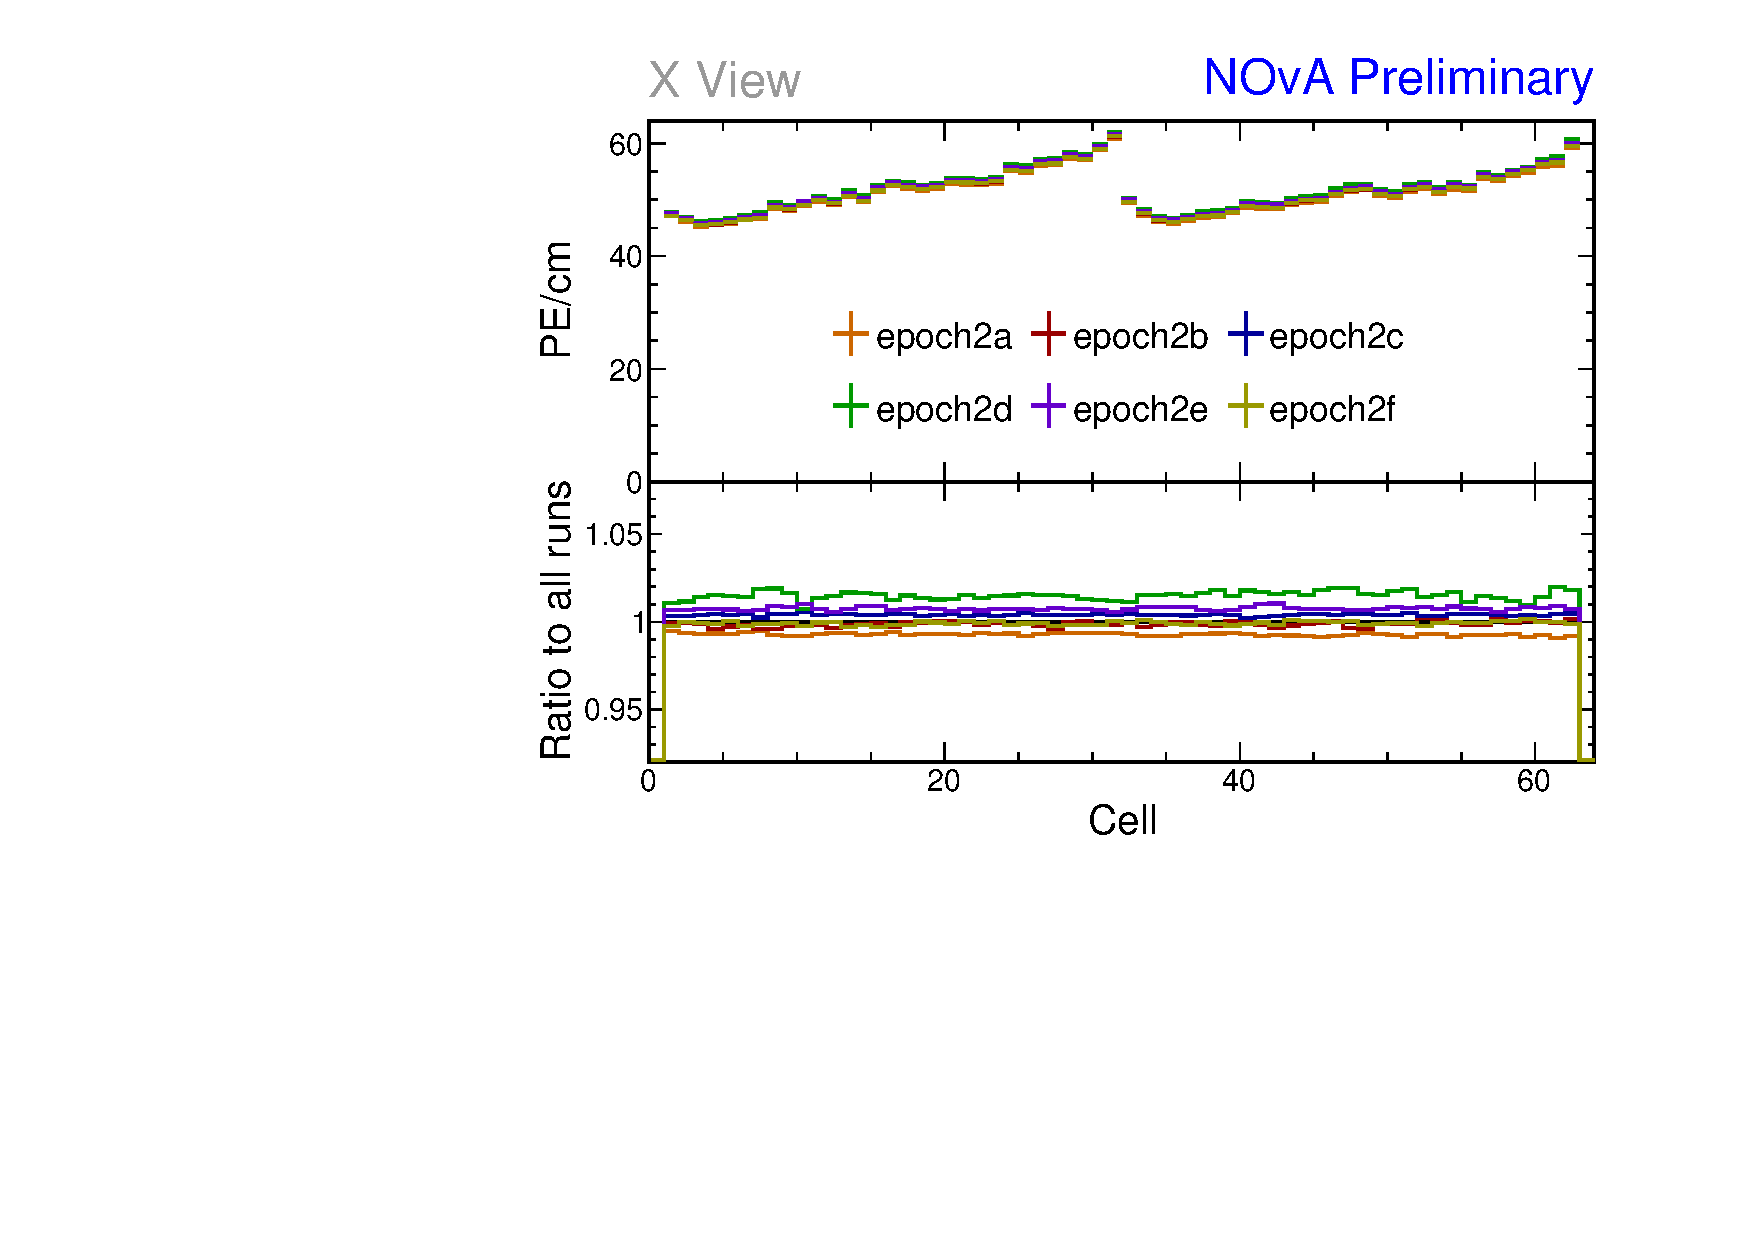
\includegraphics[width=\textwidth]{Plots/TBCalibration/Attenprofs_P2Data_CellPE_X_Combined.pdf}
\end{subfigure}
\begin{subfigure}[b]{0.495\textwidth}
\centering
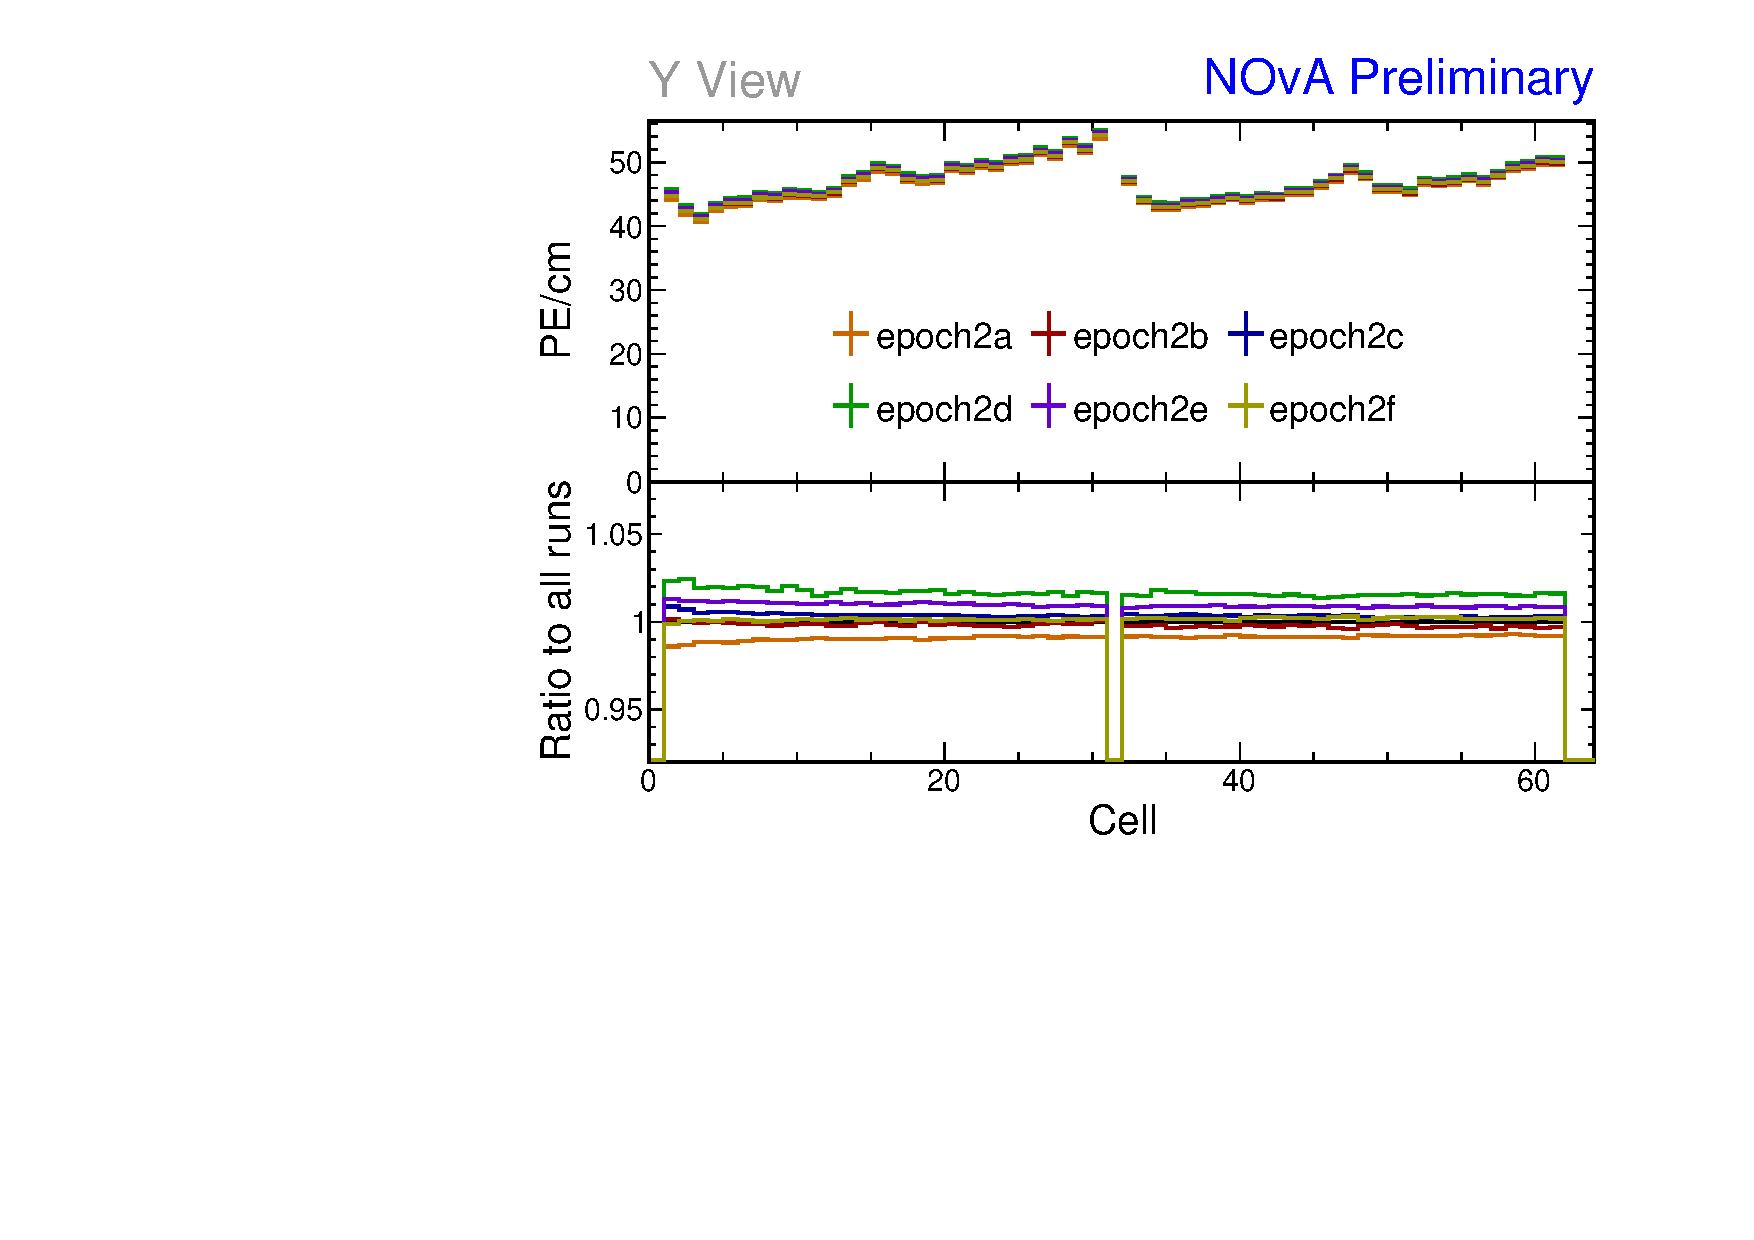
\includegraphics[width=\textwidth]{Plots/TBCalibration/Attenprofs_P2Data_CellPE_Y_Combined.pdf}
\end{subfigure}
\caption{Uncorrected energy response along cells for epochs in period 2 data.}
\label{fig:CalibhistCellPE_period2}
\end{figure}

The only variation of energy response in shape can be seen on the distributions along planes in Fig.~\ref{fig:CalibhistPlanePE_period2}. Here, in the top panel of the right plot, we can see that the uncorrected response in plane 55 is noticeably higher than the rest of the detector. The exact reason for this is unknown, but it is likely caused by a fault in one of the two \gls{FEB}s that make up the plane readout.

\begin{figure}[h]
\centering
\begin{subfigure}[b]{0.495\textwidth}
\centering
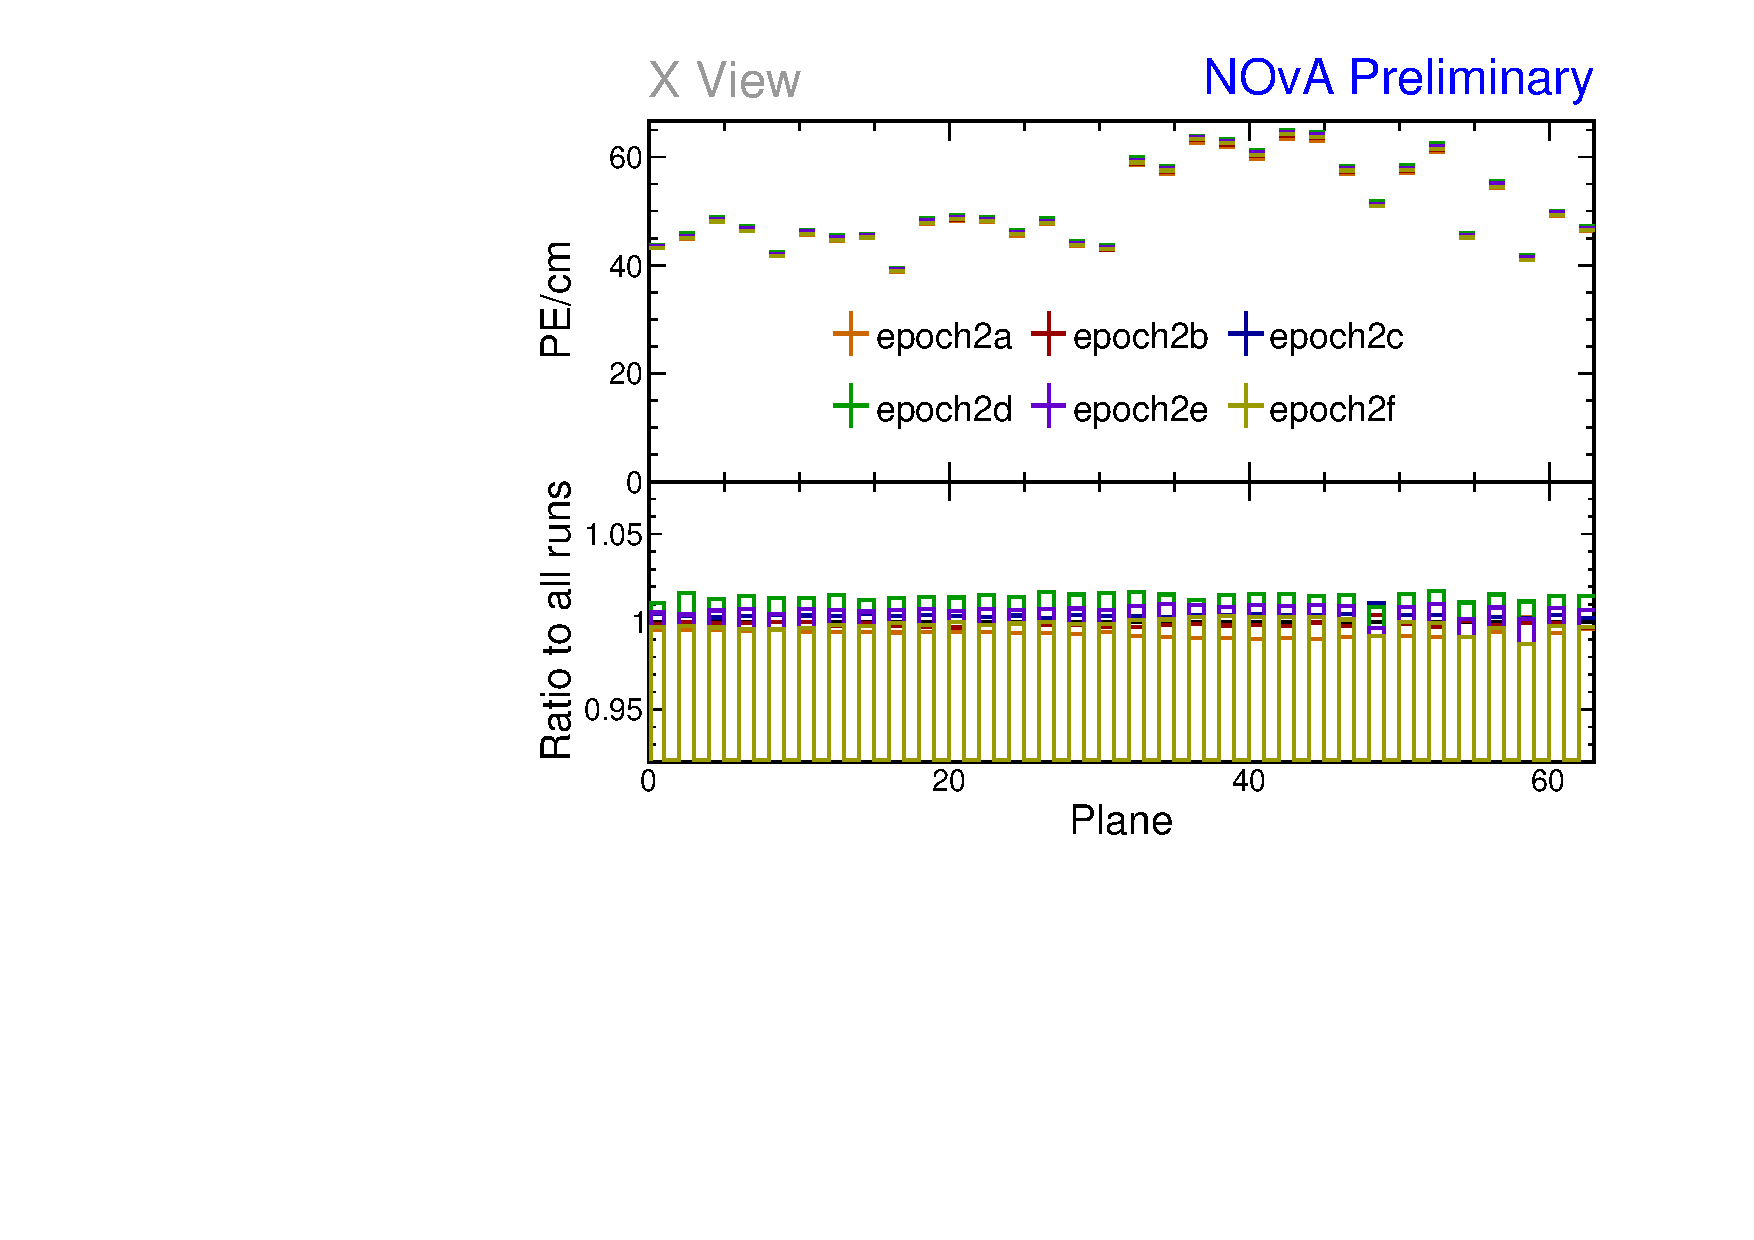
\includegraphics[width=\textwidth]{Plots/TBCalibration/Attenprofs_P2Data_PlanePE_X_Combined.pdf}
\end{subfigure}
\begin{subfigure}[b]{0.495\textwidth}
\centering
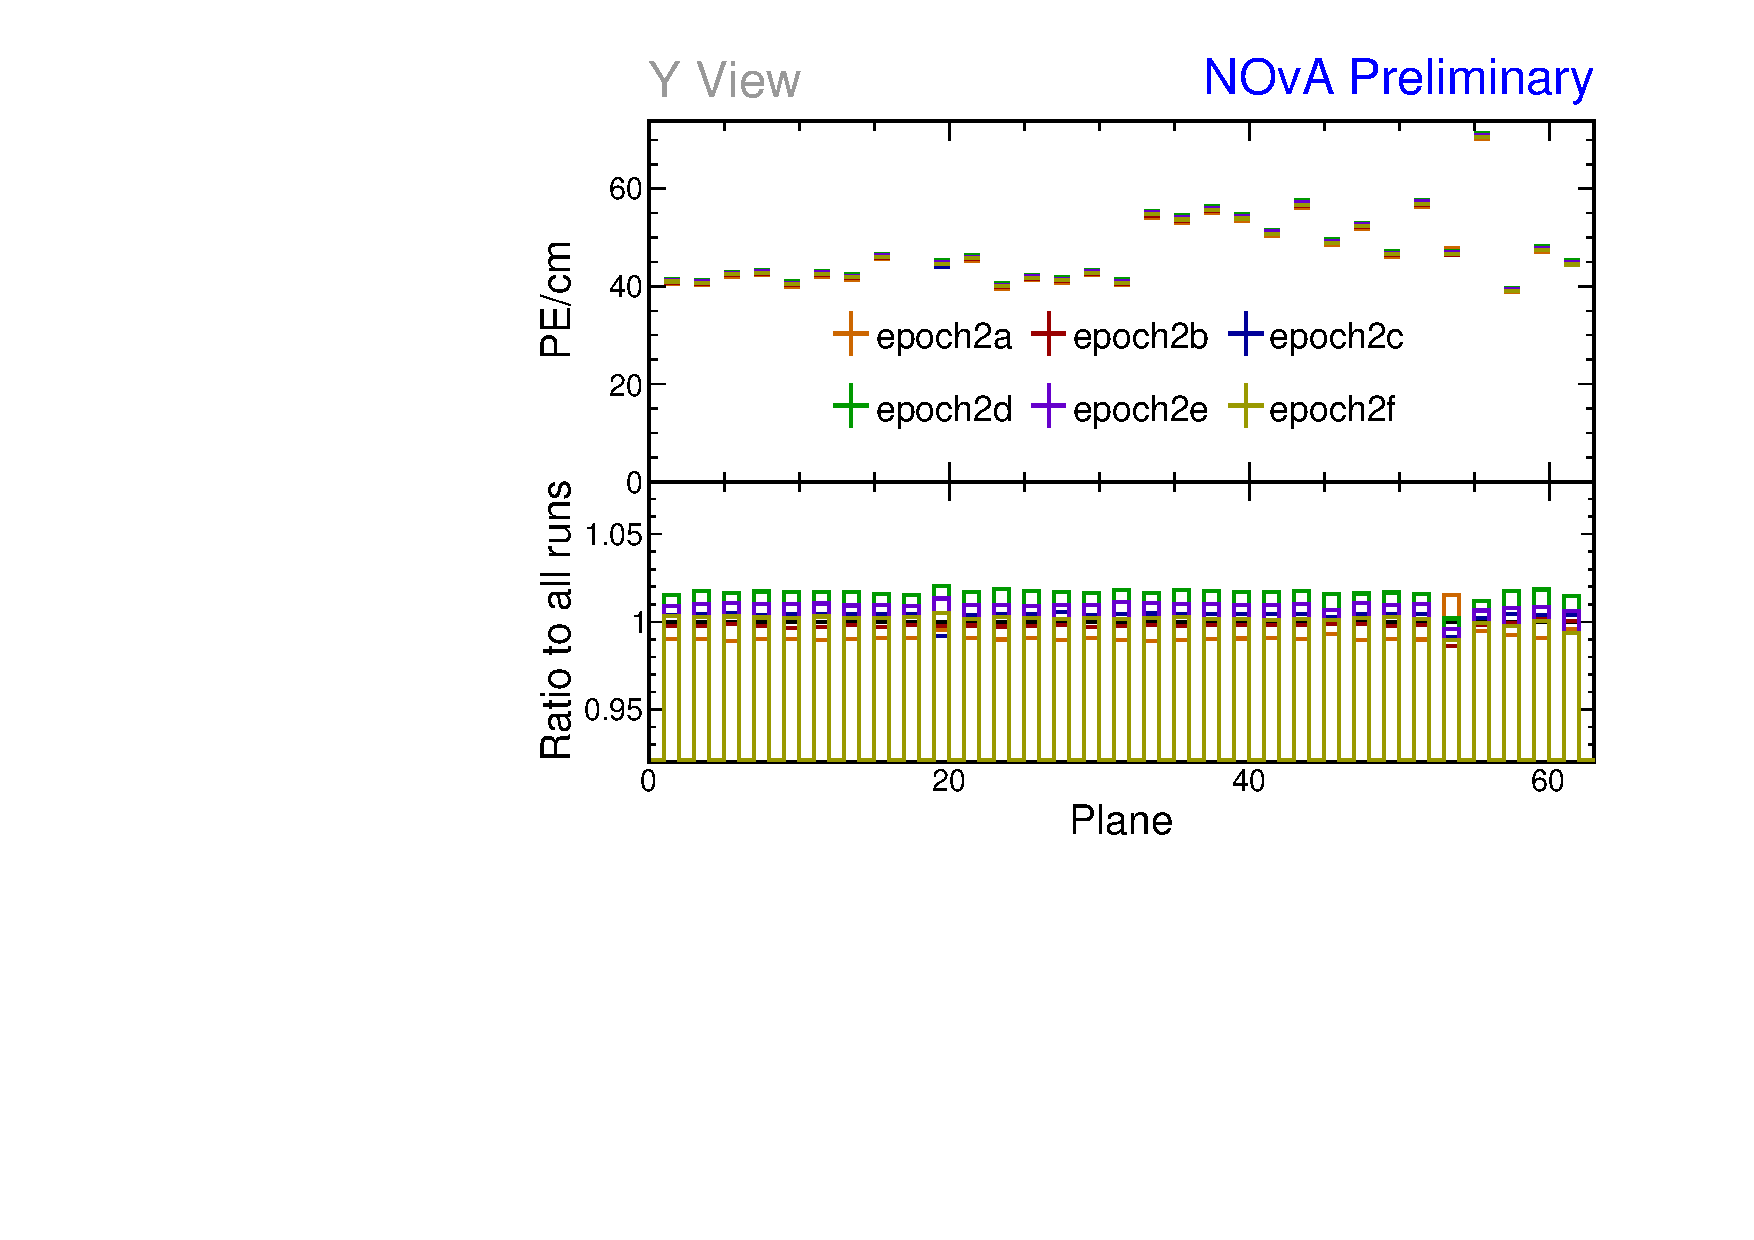
\includegraphics[width=\textwidth]{Plots/TBCalibration/Attenprofs_P2Data_PlanePE_Y_Combined.pdf}
\end{subfigure}
\caption{Uncorrected average energy response along planes for epochs in period 2 data.}
\label{fig:CalibhistPlanePE_period2}
\end{figure}

\subsubsection*{Period 2 Relative Calibration Results}

The results of the attenuation fit for period 2 are summarised in Fig.~\ref{fig:CellCentreResponsePeriod2}, showing the map of the fitted response at the centre of each cell. Same as for simulation, the blank cells failed the calibration condition for the attenuation fit. There are 199 cells that failed the calibration condition out of the total 4032 cells, constituting 4.94\% of the detector left uncalibrated for period 2.

\begin{figure}[h]
\centering
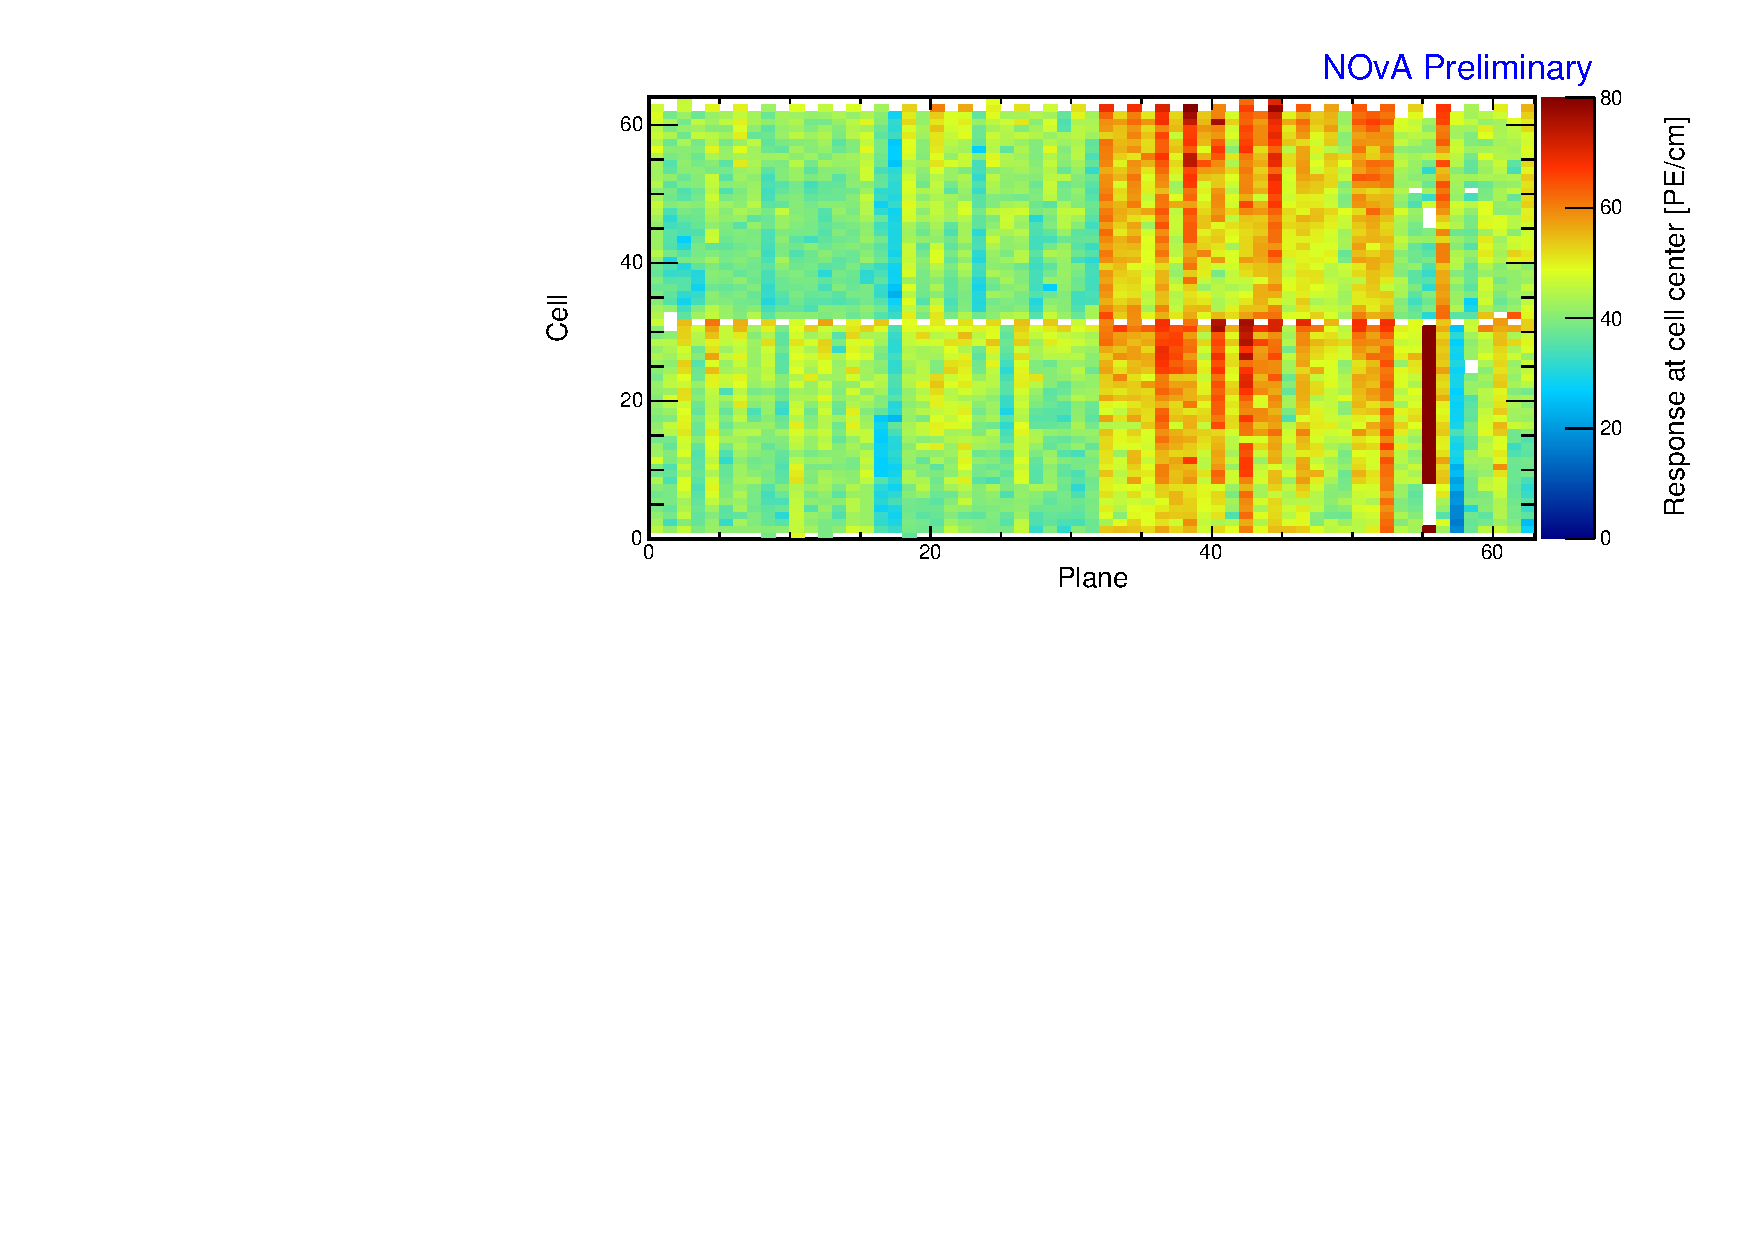
\includegraphics[width=\textwidth]{Plots/TBCalibration/CellResponseAtCentre_period2_Limited_NOvAPlotStyle.pdf}
\caption[Map of fitted response at cell centre for period 2 data]{Overview of the relative calibration results for the Test Beam detector period 2 data. Each cell represents the result of the attenuation fit to the energy response in the centre of that cell. The blank cells are uncalibrated.}
\label{fig:CellCentreResponsePeriod2}
\end{figure}

Most of the cells have an expected response, with steady rise towards the readout and a drop on the edges, as shown on the left plot of Fig.~\ref{fig:AttenfitResultsPerio2_ZippedFibers}. This is the same as was shown for simulation.

\begin{figure}[h]
  \begin{subfigure}{0.495\textwidth}
    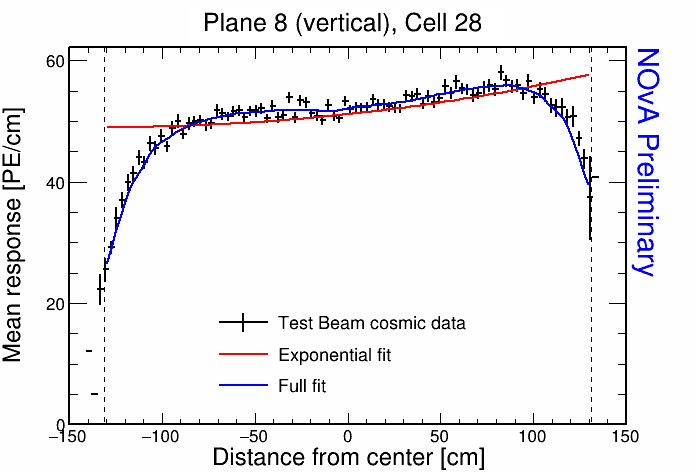
\includegraphics[width=\linewidth]{Plots/RelativeCalibrationResults/p2_008_028.png}
  \end{subfigure}
  \begin{subfigure}{0.495\textwidth}
    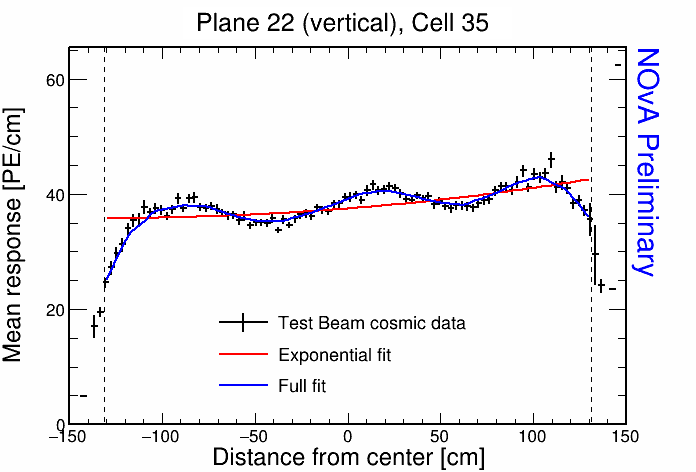
\includegraphics[width=\linewidth]{Plots/RelativeCalibrationResults/p2_022_035.png}
  \end{subfigure}
  \caption[Attenuation fits for standard cells in period 2 data]{Attenuation fits for a selection of cells in period 2. Left plot shows an example of the standard energy deposition in the Test Beam. Right plot shows the effect of zipped fibres.}
  \label{fig:AttenfitResultsPerio2_ZippedFibers}
\end{figure}

Some cells have a non-regular response across the cell, with one or more regions with a drop in the energy response, as shown on the right plot of Fig.~\ref{fig:AttenfitResultsPerio2_ZippedFibers}. These low regions are (almost certainly) a real physical effect caused by zipped, or possibly even twisted, \gls{WLS} fibres \cite{NOvA-doc-43249}. This effect is present in all the \gls{NOvA} detectors. As can be seen, the attenuation fit is capable of fitting this response and therefore the relative calibration corrects for this effect in data. However, zipped fibres are not included in simulation for any of the detectors, which could potentially cause issues with the \gls{ADC} threshold in simulation. It was decided that this is not does not have a significant impact and it would not be worth the amount of work required to include all the zipped fibres into the simulation.

Since the underfilled cells were marked as bad channels, we didn't attempt to calibrate them. Their neighbours have fewer events due to the tricell condition, but majority of them pass the calibration condition, as shown in Fig.~\ref{fig:AttenfitResultsPerio2_UnderfilledCells}. The decision to mark the underfilled cells as bad channel was motivated by the fact that bad channels get skipped by the tricell condition and the neighbouring cells to the underfilled cells can therefore be included in calibration. The fact that majority of the neighbouring cells to the underfilled cells do get calibrated clearly proves that this was a good decision.

\begin{figure}[h]
  \begin{subfigure}{0.495\textwidth}
    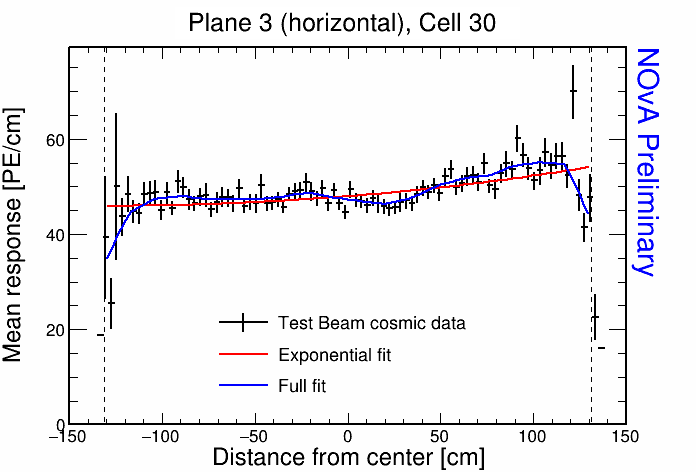
\includegraphics[width=\linewidth]{Plots/RelativeCalibrationResults/p2_003_030.png}
  \end{subfigure}
  \begin{subfigure}{0.495\textwidth}
    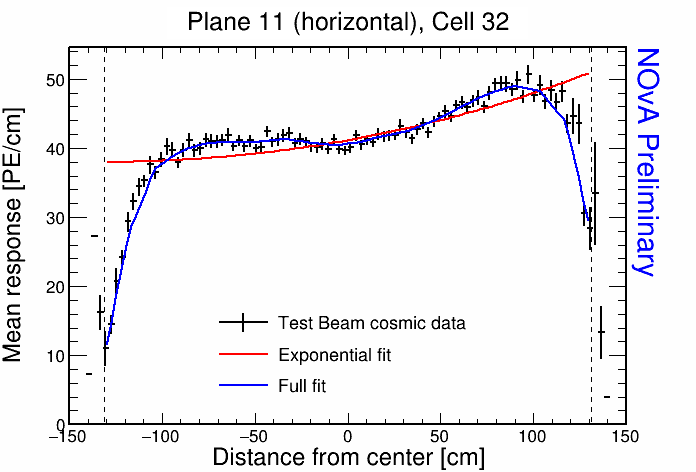
\includegraphics[width=\linewidth]{Plots/RelativeCalibrationResults/p2_011_032.png}
  \end{subfigure}
  \caption[Attenuation fits for underfilled cells in period 2 data]{Fit to the energy response in period 2. The cells neighbouring the underfilled cells have fewer events and therefore larger fluctuations than the `usual' Test Beam cell.}
  \label{fig:AttenfitResultsPerio2_UnderfilledCells}
\end{figure}

The neighbouring cells in plane 1 don't pass the calibration condition due to low statistics and therefore large fluctuations, as shown in Fig.~\ref{fig:AttenfitResultsPerio2_UnderfilledCellsPlane01}. This is likely due to a combination of the tricell condition and plane 1 being on the edge of the detector, which typically has fewer (accepted) hits than the center, as shown in Fig.~\ref{fig:Calibhist_period2}.

\begin{figure}[h]
  \begin{subfigure}{0.495\textwidth}
    \includegraphics[width=\linewidth]{Plots/RelativeCalibrationResults/p2_001_030.png}
  \end{subfigure}
  \begin{subfigure}{0.495\textwidth}
    \includegraphics[width=\linewidth]{Plots/RelativeCalibrationResults/p2_001_032.png}
  \end{subfigure}
  \caption[Attenuation fits for underfilled cells in plane 1 in period 2 data]{Fit to the energy response in period 2. The neighbouring cells to the underfilled cells in plane 1 are uncalibrated due to low statistics.}
  \label{fig:AttenfitResultsPerio2_UnderfilledCellsPlane01}
\end{figure}

The left half of plane 55 has more than $3\times$ larger response than the surrounding planes, as shown on the left plot of Fig.~\ref{fig:AttenfitResultsPerio2_FaultyFEB}. Similarly, the left half of plane 57 has slightly lower response than the surrounding planes, as shown on the right plot of Fig.~\ref{fig:AttenfitResultsPerio2_FaultyFEB}. This is due to the corresponding \gls{APD}s/\gls{FEB}s incorrectly recording a scaled up/down energy response than the real energy deposited in the detector. The cause of this scaled response is not known. Since this effect is present for all data, not only for the cosmic muons used for the calibration, it is important to correctly calibrate it out. A reason for concern is that this issue can arise if these \gls{FEB}s were only affected for a limited time out of the entire calibrated period. Since we are doing the attenuation fit on the average response across the whole calibrated period, if an \gls{FEB} records a standard response for half of the time and $7\times$ larger response for the seconds half, calibration is going to assume the response was $4\times$ larger the entire time, which would be incorrect. However, since both of the affected planes are in the back of the detector, we decided to ignore this effect for period 2.

\begin{figure}[h]
  \begin{subfigure}{0.495\textwidth}
    \includegraphics[width=\linewidth]{Plots/RelativeCalibrationResults/p2_055_011.png}
  \end{subfigure}
  \begin{subfigure}{0.495\textwidth}
    \includegraphics[width=\linewidth]{Plots/RelativeCalibrationResults/p2_057_011.png}
  \end{subfigure}
  \caption[Attenuation fits for cells in planes 55 and 57 in period 2 data]{Fit to the energy response in period 2. Lower halves of planes 55 and 57 have a different scale of energy response than the surrounding planes.}
  \label{fig:AttenfitResultsPerio2_FaultyFEB}
\end{figure}

As was discussed above, there are three dead channels with lower number of hits, possibly caused by swapped cables. These are located in planes 48 and 55. An example of one of the dead channels in plane 55 is shown on the left of Fig.~\ref{fig:AttenfitResultsPerio2_SwappedCables} together with one of the neighbouring cells on the right. As can be seen in Fig.~\ref{fig:CellCentreResponsePeriod2}, the dead channel in plane 48 and its neighbours were successfully calibrated despite the lower number of hits.

\begin{figure}[h]
  \begin{subfigure}{0.495\textwidth}
    \includegraphics[width=\linewidth]{Plots/RelativeCalibrationResults/p2_055_046.png}
  \end{subfigure}
  \begin{subfigure}{0.495\textwidth}
    \includegraphics[width=\linewidth]{Plots/RelativeCalibrationResults/p2_055_045.png}
  \end{subfigure}
  \caption[Attenuation fits for cells with swapped cables in period 2 data]{Fit to the energy response in period 2. Cells with swapped readout cables have almost no recorded events as shown on the left. This also affect their neighbouring cells due to the tricell condition as shown on the right.}
  \label{fig:AttenfitResultsPerio2_SwappedCables}
\end{figure}

Several cells in the end of the Test Beam detector are uncalibrated due to the histogram bins on the edges of the cell having an unusually high response, or no events at all, as shown in Fig.~\ref{fig:AttenfitResultsPerio2_CellEdge}. It is unknown if this is a real physical effect, possibly related to the fibres, or if it is unfiltered noise hits, issue with the binning, or something else entirely. Since these cells are in the end of the detector, we decided to ignore them.

\begin{figure}[h]
  \begin{subfigure}{0.495\textwidth}
    \includegraphics[width=\linewidth]{Plots/RelativeCalibrationResults/p2_054_050.png}
  \end{subfigure}
  \begin{subfigure}{0.495\textwidth}
    \includegraphics[width=\linewidth]{Plots/RelativeCalibrationResults/p2_058_024.png}
  \end{subfigure}
  \begin{subfigure}{0.495\textwidth}
    \includegraphics[width=\linewidth]{Plots/RelativeCalibrationResults/p2_058_025.png}
  \end{subfigure}
  \begin{subfigure}{0.495\textwidth}
    \includegraphics[width=\linewidth]{Plots/RelativeCalibrationResults/p2_060_032.png}
  \end{subfigure}
  \caption[Attenuation fits for cells with large fluctuations in period 2 data]{Fit to the energy response in period 2. Examples of cells that have an unusually high or low energy response at the edge of the cell. These cells are not calibrated.}
  \label{fig:AttenfitResultsPerio2_CellEdge}
\end{figure}

\FloatBarrier
\subsection{Period 3 Data}\label{sec:TBCalibration_period3}
The underfilled cells were refilled (or overfilled) during the period 3 data taking. This was the main motivation for dividing period 3 into individual epochs as shown on Tab.~\ref{tab:TestBeamPeriod3Epochs}. Another major event that could impact the Test Beam data is the replacement of several faulty \gls{FEB}s, which motivated the creation of epoch 3e.

\begin{table}[!ht]
\centering
\caption[Description of Test Beam period 3 epochs]{Test Beam period 3 epochs, their start dates and the reason for their separation.}
\def\arraystretch{1.4}
\begin{tabular}{m{0.11\textwidth} m{0.22\textwidth} m{0.55\textwidth}}
Name & Start date & Reason for creating the epoch\\\hline
Epoch 3a & January $12^{\textsf{th}}$ 2021 & Underfilled cells\\
Epoch 3b & April $21^{\textsf{st}}$ 2021 & Overfilling the back 9 horizontal planes and the 7th horizontal plane from the front\\
Epoch 3c & April $27^{\textsf{th}}$ 2021 & Overfilling of the 15 front horizontal planes (except the 7th, which was already done) and the 14th horizontal plane\\
Epoch 3d & April $30^{\textsf{th}}$ 2021 & Overfilling of the remaining 8 horizontal planes\\
Epoch 3e & May $12^{\textsf{th}}$ 2021 & FEB swaps
\end{tabular}
\label{tab:TestBeamPeriod3Epochs}
\end{table}

The refilling of the underfilled cells can be clearly seen on the cell hits distribution in Fig.~\ref{fig:Calibhist_period3} and on the distribution of energy deposition across horizontal cells (Y view) in Fig.~\ref{fig:CalibhistCellPE_period3}.

\begin{figure}[!hbtp]
\centering
\begin{subfigure}[b]{\textwidth}
\centering
\includegraphics[width=\textwidth]{Plots/TBCalibration/Attenprofs_P3Data_CellPlane_Epoch3a.pdf}
\end{subfigure}
\begin{subfigure}[b]{\textwidth}
\centering
\includegraphics[width=\textwidth]{Plots/TBCalibration/Attenprofs_P3Data_CellPlane_Epoch3de.pdf}
\end{subfigure}
\caption[Plane-Cell distribution of hits for the period 3 data sample]{Distribution of events in the period 3 Test Beam data calibration sample. Comparison of Epoch 3a data before the refilling of the underfilled cells and Epoch 3de (combination of Epochs 3d and 3e) after the full refilling.}
\label{fig:Calibhist_period3}
\end{figure}

\begin{figure}[hbtp]
\centering
\begin{subfigure}[b]{0.495\textwidth}
\centering
\includegraphics[width=\textwidth]{Plots/TBCalibration/Attenprofs_P3Data_WPE_corr_xy_X_Combined.pdf}
\end{subfigure}
\begin{subfigure}[b]{0.495\textwidth}
\centering
\includegraphics[width=\textwidth]{Plots/TBCalibration/Attenprofs_P3Data_WPE_corr_xy_Y_Combined.pdf}
\end{subfigure}
\caption{Uncorrected average energy response along the position within a cell for epochs in period 3 data.}
\label{fig:CalibhistWPE_period3}
\end{figure}

\begin{figure}[hbtp]
\centering
\begin{subfigure}[b]{0.495\textwidth}
\centering
\includegraphics[width=\textwidth]{Plots/TBCalibration/Attenprofs_P3Data_CellPE_X_Combined.pdf}
\end{subfigure}
\begin{subfigure}[b]{0.495\textwidth}
\centering
\includegraphics[width=\textwidth]{Plots/TBCalibration/Attenprofs_P3Data_CellPE_Y_Combined.pdf}
\end{subfigure}
\caption{Uncorrected average energy response along cells for epochs in period 3 data.}
\label{fig:CalibhistCellPE_period3}
\end{figure}

\begin{figure}[hbtp]
\centering
\begin{subfigure}[b]{0.495\textwidth}
\centering
\includegraphics[width=\textwidth]{Plots/TBCalibration/Attenprofs_P3Data_PlanePE_X_Combined.pdf}
\end{subfigure}
\begin{subfigure}[b]{0.495\textwidth}
\centering
\includegraphics[width=\textwidth]{Plots/TBCalibration/Attenprofs_P3Data_PlanePE_Y_Combined.pdf}
\end{subfigure}
\caption{Uncorrected average energy response along planes for epochs in period 3 data.}
\label{fig:CalibhistPlanePE_period3}
\end{figure}

From the cell hits distributions in Fig.~\ref{fig:Calibhist_period3} we can also see there are a few channels (cells) that were likely dead for a certain time and weren't recording the same number of events as the surrounding cells. This is specifically plane 48, cell 39 in all of period 3 and plane 18, cell 31 in epochs 3d and 3e. Cell 39 in plane 48 was also affected in period 2.

The energy distributions across cells and planes in the X view (vertical) in Fig.~\ref{fig:CalibhistCellPE_period3} and \ref{fig:CalibhistPlanePE_period3} shows, that the top half of plane 58 has a very distinctly different energy deposition compared to the rest of the cells. Specifically, that the energy response in this module was larger in epoch 3a, then got lower in epochs 3b and 3c, until getting significantly lower for epochs 3d and 3e. However, Fig.~\ref{fig:Calibhist_period3} shows that module has the same number of events as the surrounding modules. This is one of the \gls{FEB} that got replaced between epochs 3d and 3e. and as will be shown below this is the \gls{FEB} with the largest impact on the calibration out of the faulty \gls{FEB}s replaced before the start of epoch 3e.

From the aforementioned considerations, we decided to calibrate epochs 3a, 3b and 3c together, which are all the epochs containing any underfilled cells, and to separately calibrate epochs 3d and 3e together. The faulty \gls{FEB} in the top of plane 58 is far enough in the back of the detector, that we didn't find it necessary to calibrate epochs 3d and 3e separately. Also epochs 3b and 3c only contain a few days worth of data, therefore they wouldn't have enough statistics for a successful attenuation fit.

\subsubsection*{Combined Epochs 3a, 3b and 3c Relative Calibration Results}

The results of the attenuation fit for the combined epochs 3a, 3b and 3c are summarised in Fig.~\ref{fig:CellCentreResponseEp3abc}, showing the map of the fitted response at the centre of each cell. There are 182 uncalibrated cells out of 4032, constituting 4.51\% of the detector.

\begin{figure}[!hbtp]
\centering
\includegraphics[width=\textwidth]{Plots/TBCalibration/CellResponseAtCentre_epoch3abc_Limited_NOvAPlotStyle.pdf}
\caption[Map of fitted response at cell centre for epochs 3a, 3b and 3c data]{Overview of the relative calibration results for the Test Beam detector period 3, combined epochs 3a, 3b and 3c data. Each cell represents the result of the attenuation fit to the energy response in the centre of that cell. The blank cells are uncalibrated.}
\label{fig:CellCentreResponseEp3abc}
\end{figure}

We can see that some of the underfilled cells that have been refilled for epochs 3b or 3c, but were underfilled for epoch 3a which makes up the majority of this calibrated data, are now calibrated thanks to including these two short epochs into the same attenuation fit. An example of energy deposition in such a cell is on the left side of Fig.~\ref{fig:AttenfitResultsEpoch3abc_UnderfilledCellsNeighbours}.

\begin{figure}[h]
  \begin{subfigure}{0.495\textwidth}
    \includegraphics[width=\linewidth]{Plots/RelativeCalibrationResults/ep3abc_005_031.png}
  \end{subfigure}
  \begin{subfigure}{0.495\textwidth}
    \includegraphics[width=\linewidth]{Plots/RelativeCalibrationResults/ep3abc_001_032.png}
  \end{subfigure}
  \caption[Attenuation fits for re-filled cells in period 3 data]{Fit to the energy response in epochs 3a, 3b and 3c. Some underfilled cells that have been refilled in epochs 3b and 3c are now calibrated as shown on the left plot. Cell 32 in plane 1 is the only neighbouring cell to the underfilled cell that didn't manage to get calibrated due to low number of events.}
  \label{fig:AttenfitResultsEpoch3abc_UnderfilledCellsNeighbours}
\end{figure}

Same as in period 2, most of the neighbouring cells to the underfilled cells are calibrated, except for cell 32 in plane 1, shown on the right of Fig.~\ref{fig:AttenfitResultsEpoch3abc_UnderfilledCellsNeighbours}. This is due to the low statistics at the edges of the detector, same as in period 2.

There is a couple of notably faulty \gls{FEB}s with a different energy response than their neighbours. Besides the expected top half of plane 58, which has about $5\times$ larger response than the usual, there is also the top half of plane 36, which has about $2.5\times$ larger response as its neighbours. This could mean that the \gls{FEB} in plane 36 was faulty only for a limited time compared to the \gls{FEB} in plane 58. This is a reason for concern, as this could mean that using the results of this attenuation fit for hits in this module when the \gls{FEB} wasn't faulty would give an incorrectly large correction (and therefore small `corrected response'), whereas hits during the period when the \gls{FEB} was faulty would have smaller than required correction (and therefore larger corrected response). Given that plane 36 is in the middle of the detector, this might affect some Test Beam analysis results. It is possible this might have to be mitigated in the future, whether with an additional uncertainty, or by improving the calibration. \note{Should I talk about this further? We decided not to correct this since it would take more time and it might not be a huge problem. But this is probably the most problematic part of the calibration}. The energy deposition for these cells is shown in Fig.~\ref{fig:AttenfitResultsEpoch3abc_FaultyFEBs}. As plane 58 is in the end of the detector and its readout was likely faulty for the majority of the calibrated period, we decided to ignore this \gls{FEB}.

\begin{figure}[h]
  \begin{subfigure}{0.495\textwidth}
    \includegraphics[width=\linewidth]{Plots/RelativeCalibrationResults/ep3abc_036_054.png}
  \end{subfigure}
  \begin{subfigure}{0.495\textwidth}
    \includegraphics[width=\linewidth]{Plots/RelativeCalibrationResults/ep3abc_058_048.png}
  \end{subfigure}
  \caption[Attenuation fits for cells with faulty readout in period 3 data]{Fit to the energy response in epochs 3a, 3b and 3c. The most obvious faulty FEBs that have a significantly larger energy response than their neighbours.}
  \label{fig:AttenfitResultsEpoch3abc_FaultyFEBs}
\end{figure}

Similarly to period 2, there are a few cell in the back of the detector that have a sharp rise in the energy response at the edge of the cell, which causes thee attenuation fit to fail the calibration condition. This can be seen in Fig.~\ref{fig:AttenfitResultsEpoch3abc_CellEdges} with significantly different mean responses at the edge bins pulling the attenuation fit to incorrect values. Given this is happening only in the end of the detector, we decided it should be safe to ignore this effect.

\begin{figure}[h]
  \begin{subfigure}{0.495\textwidth}
    \includegraphics[width=\linewidth]{Plots/RelativeCalibrationResults/ep3abc_058_002.png}
  \end{subfigure}
  \begin{subfigure}{0.495\textwidth}
    \includegraphics[width=\linewidth]{Plots/RelativeCalibrationResults/ep3abc_060_032.png}
  \end{subfigure}
  \caption[Attenuation fits for cells with large fluctuations in period 3 data]{Fit to the energy response in epochs 3a, 3b and 3c. Some cells are not calibrated due to large fluctuations at one edge of the cells.}
  \label{fig:AttenfitResultsEpoch3abc_CellEdges}
\end{figure}

\subsubsection*{Combined Epochs 3d and 3e Relative Calibration Results}

The results of the attenuation fits for epochs 3d and 3e are shown in Fig.~\ref{fig:CellCentreResponseEp3de}. There are 182 uncalibrated cells out of 4032 total cells, making up 4.51\% of the detector. The uncalibrated are now however almost entirely concentrated at the edges and at the end of the detector.

\begin{figure}[!hbtp]
\centering
\includegraphics[width=\textwidth]{Plots/TBCalibration/CellResponseAtCentre_epoch3de_original_Limited_NOvAPlotStyle.pdf}
\caption[Map of fitted response at cell centre for epochs 3d and 3e data]{Overview of the relative calibration results for the Test Beam detector period 3, combined epochs 3d and 3e data. Each cell represents the result of the attenuation fit to the energy response in the centre of that cell. The blank cells are uncalibrated.}
\label{fig:CellCentreResponseEp3de}
\end{figure}

Figure~\ref{fig:CellCentreResponseEp3de} shows the expected uncalibrated cells in plane 17 surrounding the dead channel discussed above (or possible still an underfilled cell). The energy deposition for this cell and one of its neighbours is shown in Fig.~\ref{fig:AttenfitResultsEpoch3de_LeftoverUnderfilledCell}.

\begin{figure}[h]
  \begin{subfigure}{0.495\textwidth}
    \includegraphics[width=\linewidth]{Plots/RelativeCalibrationResults/ep3de_017_031.png}
  \end{subfigure}
  \begin{subfigure}{0.495\textwidth}
    \includegraphics[width=\linewidth]{Plots/RelativeCalibrationResults/ep3de_017_032.png}
  \end{subfigure}
  \caption[Attenuation fits for dead channels cells in period 3 data]{Fit to the energy response in epochs 3d and 3e. Possibly dead channel or still underfilled cell.}
  \label{fig:AttenfitResultsEpoch3de_LeftoverUnderfilledCell}
\end{figure}

Epochs 3d and 3e should have all the previously underfilled cells now refilled, but as can be seen in Fig. \ref{fig:CellCentreResponseEp3de}, there's several of these cells that are still uncalibrated. The energy deposition in these cells is shown in Fig.~\ref{fig:AttenfitResultsEpoch3de_RefilledDiscrepancy}. Here we can see, that these cells have a fairly large discrepancy between the left and right side of the cells. This is caused by using different scintillator oils for the initial filling of the cells and for the refilling. Specifically, as was described in Sec.~\ref{sec:TBExperiment}, these cells have been initially filled with the Ash River and the Texas oils, which have higher energy depositions compared to the \gls{NDOS} oil that was used for the refilling during period 3. These oils clearly didn't mix properly, which caused a difference in energy deposition in different parts of the cells.

\begin{figure}[h]
  \begin{subfigure}{0.495\textwidth}
    \includegraphics[width=\linewidth]{Plots/RelativeCalibrationResults/ep3de_033_031.png}
  \end{subfigure}
  \begin{subfigure}{0.495\textwidth}
    \includegraphics[width=\linewidth]{Plots/RelativeCalibrationResults/ep3de_059_031.png}
  \end{subfigure}
  \caption[Attenuation fits for cells with mixed scintillators in period 3 data]{Fit to the energy response in epochs 3d and 3e. The scintillator oil used for refilling of the underfilled cells has lower energy response than the oil used for the initial filling. These oils didn't mix properly causing a different energy response in the left and right side of the cell.}
  \label{fig:AttenfitResultsEpoch3de_RefilledDiscrepancy}
\end{figure}

This is a physical effect that should be accounted for in the calibration and as we can see, the attenuation fits are actually performing reasonably well. Additionally, these cells are in the middle of the detector and leaving them uncalibrated would almost certainly have an impact on the Test Beam analyses. The large $\chi^2$ value of the attenuation fit is most likely caused only by the unusual shape of the distribution, which the fit is not designed for. We have therefore decided to manually change the $\chi^2$ values for these cells inside the cvs tables (which hold the results of the attenuation fits), so that their $\chi^2<0.2$ and these cells are officially considered calibrated, even if they originally weren't. The `corrected' distribution of the attenuation fit results for epochs 3d and 3e is shown in Fig.~\ref{fig:CellCentreResponseEp3de_updated}. The number of uncalibrated cells was reduced by 8 to 174, or 4.32\% of the detector.

\begin{figure}[!hbtp]
\centering
\includegraphics[width=\textwidth]{Plots/TBCalibration/CellResponseAtCentre_epoch3de_Limited_NOvAPlotStyle.pdf}
\caption[Corrected map of fitted response at cell centre for epochs 3d and 3e data]{Overview of the relative calibration results for the Test Beam detector period 3, combined epochs 3d and 3e data. Each cell represents the result of the attenuation fit to the energy response in the centre of that cell. The blank cells are uncalibrated. The previously uncalibrated cells in the middle of the detector were artificially marked as calibrated after careful considerations.}
\label{fig:CellCentreResponseEp3de_updated}
\end{figure}

Some of the cells in the back of the detector have a rise, or drop in energy deposition at the edge of the cell, as can be seen in Fig.~\ref{fig:AttenfitResultsEpoch3de_CellEdges}. This is similar to the effect seen in period 2 and epochs 3a+3b+3c and since it's again concentrated in the end of the detector, we ignored these cells and left them uncalibrated.

\begin{figure}[h]
  \begin{subfigure}{0.495\textwidth}
    \includegraphics[width=\linewidth]{Plots/RelativeCalibrationResults/ep3de_050_018.png}
  \end{subfigure}
  \begin{subfigure}{0.495\textwidth}
    \includegraphics[width=\linewidth]{Plots/RelativeCalibrationResults/ep3de_062_006.png}
  \end{subfigure}
  \caption[Attenuation fits for cells with large fluctuations in period 3 data]{Fit to the energy response in epochs 3d and 3e. Some cells have a drop, or a rise of energy response at the edge of the cell. This can be cause by low statistics.}
  \label{fig:AttenfitResultsEpoch3de_CellEdges}
\end{figure}

\FloatBarrier
\subsection{Period 4 Data}\label{sec:TBPeriod4}

The period 4 Test Beam data taking period is the best data we managed to collect with almost ideal detector conditions. There are a few commissioning runs in the very beginning of period 4, which uncovered some dead channels or faulty \gls{FEB}s that were immediately fixed. These runs constitute epoch 4a, shown on the top of Fig.~\ref{fig:Calibhist_period4}. There is also a few runs during which we performed studies in which we masked parts of the detector to help with the \gls{FEB} saturation \cite{NOvA-doc-53658}, which can clearly be seen in the middle of Fig.~\ref{fig:Calibhist_period4}. Bottom part of Fig.~\ref{fig:Calibhist_period4} shows that the rest of the period 4 data does not have any noticeable faults in the distribution of hits across the detector.

\begin{figure}[!hbtp]
\centering
\begin{subfigure}[b]{\textwidth}
\centering
\includegraphics[width=\textwidth]{Plots/TBCalibration/Attenprofs_P4Data_CellPlane_Epoch4a.pdf}
\end{subfigure}
\begin{subfigure}[b]{\textwidth}
\centering
\includegraphics[width=\textwidth]{Plots/TBCalibration/Attenprofs_P4Data_CellPlane_CellMasking.pdf}
\end{subfigure}
\begin{subfigure}[b]{\textwidth}
\centering
\includegraphics[width=\textwidth]{Plots/TBCalibration/Attenprofs_P4Data_CellPlane_GoodRuns.pdf}
\end{subfigure}
\caption[Plane-Cell distribution of hits for the period 4 data sample]{Distribution of events in the Test Beam period 4 data calibration sample. The top plot shows the first three commissioning runs, the middle plot the status of the detector during the Cell Masking studies and the bottom plot shows the rest.}
\label{fig:Calibhist_period4}
\end{figure}

Figures \ref{fig:CalibhistWPE_period4}, \ref{fig:CalibhistCellPE_period4} and \ref{fig:CalibhistPlanePE_period4} show that the epoch 4a and the cell masking study did have a noticeable impact on the energy deposition across the detector. Both of these special periods only span a short time and contain a very limited number of hits. We therefore decided to ignore these runs and only calibrate the rest of the period 4 data, using these results for all runs in period 4. \note{I assume here that the runs from the cell masking studies will not be used in the TB analyses. Is that correct?}

\begin{figure}[!hbtp]
\centering
\begin{subfigure}[b]{0.495\textwidth}
\centering
\includegraphics[width=\textwidth]{Plots/TBCalibration/Attenprofs_P4Data_WPE_corr_xy_X_Combined.pdf}
\end{subfigure}
\begin{subfigure}[b]{0.495\textwidth}
\centering
\includegraphics[width=\textwidth]{Plots/TBCalibration/Attenprofs_P4Data_WPE_corr_xy_Y_Combined.pdf}
\end{subfigure}
\caption{Uncorrected average energy response along the position within a cell (w) for epochs in period 4 data.}
\label{fig:CalibhistWPE_period4}
\end{figure}

\begin{figure}[!hbtp]
\centering
\begin{subfigure}[b]{0.495\textwidth}
\centering
\includegraphics[width=\textwidth]{Plots/TBCalibration/Attenprofs_P4Data_CellPE_X_Combined.pdf}
\end{subfigure}
\begin{subfigure}[b]{0.495\textwidth}
\centering
\includegraphics[width=\textwidth]{Plots/TBCalibration/Attenprofs_P4Data_CellPE_Y_Combined.pdf}
\end{subfigure}
\caption{Uncorrected average energy response along cells for epochs in period 4 data.}
\label{fig:CalibhistCellPE_period4}
\end{figure}

\begin{figure}[!hbtp]
\centering
\begin{subfigure}[b]{0.495\textwidth}
\centering
\includegraphics[width=\textwidth]{Plots/TBCalibration/Attenprofs_P4Data_PlanePE_X_Combined.pdf}
\end{subfigure}
\begin{subfigure}[b]{0.495\textwidth}
\centering
\includegraphics[width=\textwidth]{Plots/TBCalibration/Attenprofs_P4Data_PlanePE_Y_Combined.pdf}
\end{subfigure}
\caption{Uncorrected average energy response along planes for epochs in period 4 data.}
\label{fig:CalibhistPlanePE_period4}
\end{figure}

\subsubsection*{Period 4 Relative Calibration Results}

Results of the attenuation fits for period 4 are summarised in Fig.~\ref{fig:CellCentreResponsePeriod4}. We can see that almost the entire detector is now calibrated. The only exceptions consists of cells on the edge of the detector, 7 formerly underfilled cells (left plot in Fig.~\ref{fig:AttenfitResultsPeriod4}), and one cell 47 in plane 54 with an unusually high response at the edge of the cell (right plot in Fig.~\ref{fig:AttenfitResultsPeriod4}).

\begin{figure}[!hbtp]
\centering
\includegraphics[width=\textwidth]{Plots/TBCalibration/CellResponseAtCentre_period4_original_Limited_NOvAPlotStyle.pdf}
\caption[Map of fitted response at cell centre for period 4 data]{Overview of the relative calibration results for the Test Beam detector period 4 data. Each cell represents the result of the attenuation fit to the energy response in the centre of that cell. The blank cells are uncalibrated.}
\label{fig:CellCentreResponsePeriod4}
\end{figure}

\begin{figure}[h]
  \begin{subfigure}{0.495\textwidth}
    \includegraphics[width=\linewidth]{Plots/RelativeCalibrationResults/p4_035_031.png}
  \end{subfigure}
  \begin{subfigure}{0.495\textwidth}
    \includegraphics[width=\linewidth]{Plots/RelativeCalibrationResults/p4_054_047.png}
  \end{subfigure}
  \caption[Attenuation fits for cells with in period 4 data]{Fit to the energy response in period 4. Previously underfilled cells refilled with a scintillator of a different quality causing an unusual distribution of energy deposition (left). Unusually high energy response at the edge of the cell 47 (right).}
  \label{fig:AttenfitResultsPeriod4}
\end{figure}

We treated the formerly underfilled cells the same way as in epochs 3d and 3e, by manually changing the $\chi^2$ of their attenuation fits inside the csv files to be $<0.2$ and therefore making them officially calibrated. The `corrected' distribution of the relative calibration results is shown in Fig.~\ref{fig:CellCentreResponsePeriod4_updated}. There are 108 uncalibrated cells out of 4032, totalling 2.68\% of the detector, almost exclusively on the edges.

\begin{figure}[!hbtp]
\centering
\includegraphics[width=\textwidth]{Plots/TBCalibration/CellResponseAtCentre_period4_Limited_NOvAPlotStyle.pdf}
\caption[Corrected map of fitted response at cell centre for period 4 data]{Overview of the relative calibration results for the Test Beam detector period 4 data. Each cell represents the result of the attenuation fit to the energy response in the centre of that cell. The blank cells are uncalibrated. The previously uncalibrated cells in the middle of the detector were artificially marked as calibrated after careful considerations.}
\label{fig:CellCentreResponsePeriod4_updated}
\end{figure}

\FloatBarrier

\newpage

\begin{center}
\begin{Huge}
\vspace*{3cm}
End of the current version of the thesis!\\[2cm]
Anything after this point was simply copied from the technote and hasn't been review yet
\end{Huge}
\end{center}

\newpage

%%%%%%%%%%%%%%%%%%%%%%%%%%%%%%%%%%%%%%%%%%%%%%%%%%%%%%%%%%%%%%%%%%%%%%%%%%%%%%%
%%%%%%%%%%%%%%%%%%%%%%%%%%%%%%%%%%%%%%%%%%%%%%%%%%%%%%%%%%%%%%%%%%%%%%%%%%%%%%%
%%%
%%%                        Absolute calibration results
%%%
%%%%%%%%%%%%%%%%%%%%%%%%%%%%%%%%%%%%%%%%%%%%%%%%%%%%%%%%%%%%%%%%%%%%%%%%%%%%%%%
\subsection{Absolute Calibration Results}
As was described in Sec.~\ref{sec:NOvACalibration}, we apply the relative calibration results on the stopping muon sample and use the absolute calibration cuts to select only well-understood minimum ionising muons. These events represent a very well understood source of energy deposition we use as a standard candle to calculate the absolute energy scale. The absolute calibration cuts are mostly the same as for the other \gls{NOvA} detectors, selecting hits $1-\unit[2]{m}$ from the end of their tracks and removing uncalibrated and wrongly reconstructed hits by requiring non-zero pathlength, $\gls{PE}>0$, and $\gls{PECorr} > 0$, as well as $\gls{PECorr}\unit{/cm} < 100$. To remove hits at the edge of the cells, we require that $-80<w<\unit[80]{cm}$, therefore removing hits approximately $\unit[0.5]{m}$ from each side of the detector.

The distributions of the reconstructed and true energy responses, for both views, and for each data and simulation sample, are shown in Fig.~\ref{fig:AbsCalibNHitsMEU}. The means of these distributions are the $\gls{MEU}_{Reco}$ and $\gls{MEU}_{True}$ values for each view. The uncertainty on the means are calculated as the standard deviation of the distributions divided by the square root of the number of entries. We average the two \gls{MEU} values from both views and combine the uncertainties in the sum of squares. The total number of entries, the \gls{MEU} values for each sample and view, and the combined \gls{MEU} values with corresponding uncertainties are shown in Tab.~\ref{tab:calib_summary_table}. Given the large number of entries in the energy response distributions, the total uncertainties on the \gls{MEU} values are negligible (around $0.05\%$). This are however not the final uncertainties of the absolute energy scale used in \gls{NOvA}. Instead, we use comparison to other standard candles, as was explained in Sec.~\ref{sec:NOvASystematics}.

\begin{figure}[ht!]
  \begin{subfigure}{\textwidth}
    \centering
    \includegraphics[height=0.2\linewidth]{essentialsec_tb/legend.pdf}
  \end{subfigure}
  \vspace*{2mm}

  \begin{subfigure}{0.495\textwidth}
    \includegraphics[width=\linewidth]{essentialsec_tb/nhits_meu_x.pdf}
  \end{subfigure}
  \begin{subfigure}{0.495\textwidth}
    \includegraphics[width=\linewidth]{essentialsec_tb/nhits_meu_y.pdf}
  \end{subfigure}
  \begin{subfigure}{0.495\textwidth}
    \includegraphics[width=\linewidth]{essentialsec_tb/nhits_mev_x.pdf}
  \end{subfigure}
  \begin{subfigure}{0.495\textwidth}
    \includegraphics[width=\linewidth]{essentialsec_tb/nhits_mev_y.pdf}
  \end{subfigure}
  \caption[Reconstructed and true energy response of stopping muons]{Distributions of the reconstructed (top) and true (bottom) energy response of stopping muons in the X (left) and Y (right) view within a $1-\unit[2]{m}$ track window from the end of their tracks. The mean of the reconstructed and true distributions of the response are the reconstructed and true MEU values respectively for the corresponding views.}
  \label{fig:AbsCalibNHitsMEU}
\end{figure}

\begin{table}[h!]
\centering
\caption[Summary of absolute calibration results]{Summary of absolute calibration results. \acrshort{MEU}$_{Reco}$ values (top table) are in units of $\gls{PECorr}\unit{/cm}$ and \acrshort{MEU}$_{True}$ values (bottom table) are in units of $\unit{MeV/cm}$}
\begin{tabular}{|c|c|c|c|c|c|c|c|}
\hline
\multicolumn{2}{|c|}{\multirow{2}{*}{Sample}} & \multicolumn{2}{c|}{X view} & \multicolumn{2}{c|}{Y view} & \multicolumn{2}{c|}{Combined}\\\cline{3-8}
\multicolumn{2}{|c|}{} & NHits & MEU & NHits & MEU & \cellcolor[HTML]{F8A102}MEU$_{Reco}$ & $\sigma_{\textsf{MEU}_{Reco}}$\\ \hline
 \parbox[t]{2mm}{\multirow{4}{*}{\rotatebox[origin=c]{90}{Data}}}
 & Period 2 & 2.322e+05 & 38.70 & 1.413e+06 & 39.40 & \cellcolor[HTML]{F8A102}39.05 & 0.02\\ \cline{2-8} 
 & Epochs 3abc & 2.638e+05 & 38.49 & 1.621e+06 & 39.40 & \cellcolor[HTML]{F8A102}38.94 & 0.02\\ \cline{2-8}
 & Epochs 3de & 1.049e+05 & 38.63 & 6.725e+05 & 39.42 & \cellcolor[HTML]{F8A102}39.02 & 0.03\\ \cline{2-8}
 & Period 4 & 5.268e+05 & 38.63 & 3.316e+06 & 39.40 & \cellcolor[HTML]{F8A102}39.01 & 0.01\\ \hline
\multicolumn{2}{|c|}{Simulation} & 2.829e+05 & 40.17 & 1.842e+06 & 39.93 & \cellcolor[HTML]{F8A102}40.05 & 0.02\\ \hline
\end{tabular}

\vspace*{2mm}
\begin{tabular}{|c|c|}
\hline
\cellcolor[HTML]{F8A102}MEU$_{True}$ = 1.7722 $\unit{MeV/cm}$ & $\sigma_{\textsf{MEU}_{True}}$ = 0.0003 $\unit{MeV/cm}$\\ \hline
\end{tabular}
\label{tab:calib_summary_table}
\end{table}

%%%%%%%%%%%%%%%%%%%%%%%%%%%%%%%%%%%%%%%%%%%%%%%%%%%%%%%%%%%%%%%%%%%%%%%%%%%%%%%
%%%%%%%%%%%%%%%%%%%%%%%%%%%%%%%%%%%%%%%%%%%%%%%%%%%%%%%%%%%%%%%%%%%%%%%%%%%%%%%
%%%
%%%                      Final results and conclusions
%%%
%%%%%%%%%%%%%%%%%%%%%%%%%%%%%%%%%%%%%%%%%%%%%%%%%%%%%%%%%%%%%%%%%%%%%%%%%%%%%%%
\subsection{Discussion}
To validate the results of the Test Beam calibration we look at the stopping muon sample used for the absolute calibration, since these events have the most consistent and reliable energy deposition.

In plots in Fig. \ref{fig:AbsCalibW1}-\ref{fig:AbsCalibDrift2} we look at distributions of variables used during the calibration, namely $PE$, $PECorr$, $Pathlength$, $PE/cm$ and $PECorr/cm$. Their distributions are over a range of variables we tried to correct the energy deposition in, namely position within a cell $w$, cell number, plane number, track angles and time.

The most important validation plots are the distributions of $PECorr/cm$, which should be completely flat. This would mean that all the deposited energy results in an equivalent recorded energy wherever and whenever in the Test Beam detector it occurred. As can be seen on the validation plots, this was successfully achieved and the $PECorr/cm$ distributions are mostly flat across all studied variables.

The distribution of $PECorr/cm$ across cells in X view in Fig. \ref{fig:AbsCalibPlane1} seems fairly scattered, however this is mostly due to the better resolution of this plot and the dispersion of the energy deposition across cells isn't large enough to constitute further investigation.

The distributions of $PECorr/cm$ across planes in the X view (Fig. \ref{fig:AbsCalibPlane1}) shows a noticeable smaller corrected energy response of stopping muons in plane 36. This means that the relative calibration over-corrected the energy response due to the through-going muons having unusually high energy response (as shown in Fig. \ref{fig:AttenfitResultsEpoch3abc_FaultyFEBs}), but not the selected stopping muons. The most likely cause is that the impacted FEB was `faulty' only for a certain period of time. In that case the corrected energy response would be correct for the period when the FEB was faulty, but would be under-estimated for the period when the FEB behaved `normally'. The $PECorr/cm$ over Plane plot shows the average over these responses.

The corrected response across planes in Y view (Fig. \ref{fig:AbsCalibPlane1}) shows a slight incline in the first half of the detector. We do not know where does this slope come from, but it is not big enough to be of concern and we decided to ignore it.

The distributions of energy deposition in time (Fig. \ref{fig:AbsCalibDrift1} and \ref{fig:AbsCalibDrift2}) show a non-trivial dependency. The detector response could be influenced by environmental factors (temperature and humidity) and by scintillator or readout ageing. Neither of these factors are well understood within NOvA and Test Beam detector could be potentially used to shine more light on this issue. However this is a topic for a separate study and is out of scope of this technical note.

Technically, we would expect the distributions of $PECorr/cm$ to also have the same \textbf{scale} for all data samples and for simulation. As can be seen on all the validation plots, the data samples have a reasonably similar scale of $PECorr/cm$, but this is noticeably different for simulation. This is caused due to the data-based simulation we are using does not have a correct energy estimation for through-going muons, which have generally underestimated energies \cite{NOVA-doc-60026}. This results in an over-estimated correction from the relative calibration. However, this is not an issue, since we only use stopping muons to calculate the absolute energy scale and stopping muons have correct energies in the new simulation.

\begin{figure}[!ht]
  \begin{subfigure}{\textwidth}
  \centering
    \includegraphics[height=0.2\linewidth]{essentialsec_tb/legend.pdf}
  \end{subfigure}
  \vspace*{2mm}
  
  \begin{subfigure}{0.495\textwidth}
    \includegraphics[width=\linewidth]{essentialsec_tb/pecm_w_x.pdf}
  \end{subfigure}
  \begin{subfigure}{0.495\textwidth}
    \includegraphics[width=\linewidth]{essentialsec_tb/pecm_w_y.pdf}
  \end{subfigure}
  \begin{subfigure}{0.495\textwidth}
    \includegraphics[width=\linewidth]{essentialsec_tb/pecorrcm_w_x.pdf}
  \end{subfigure}
  \begin{subfigure}{0.495\textwidth}
    \includegraphics[width=\linewidth]{essentialsec_tb/pecorrcm_w_y.pdf}
  \end{subfigure}
  \caption{Distributions of stopping muons within a 1-2 m track window from the end of their tracks across the position within a cell.}
  \label{fig:AbsCalibW1}
\end{figure}

\begin{figure}[!ht]
  \begin{subfigure}{\textwidth}
  \centering
    \includegraphics[height=0.2\linewidth]{essentialsec_tb/legend.pdf}
  \end{subfigure}
  \vspace*{2mm}

  \begin{subfigure}{0.495\textwidth}
    \includegraphics[width=\linewidth]{essentialsec_tb/pecm_cell_x.pdf}
  \end{subfigure}
  \begin{subfigure}{0.495\textwidth}
    \includegraphics[width=\linewidth]{essentialsec_tb/pecm_cell_y.pdf}
  \end{subfigure}
  \begin{subfigure}{0.495\textwidth}
    \includegraphics[width=\linewidth]{essentialsec_tb/pecorrcm_cell_x.pdf}
  \end{subfigure}
  \begin{subfigure}{0.495\textwidth}
    \includegraphics[width=\linewidth]{essentialsec_tb/pecorrcm_cell_y.pdf}
  \end{subfigure}
  \caption{Distributions of stopping muons within a 1-2 m track window from the end of their tracks across the cells of the detector.}
  \label{fig:AbsCalibCell1}
\end{figure}

\begin{figure}[!ht]
  \begin{subfigure}{\textwidth}
  \centering
    \includegraphics[height=0.2\linewidth]{essentialsec_tb/legend.pdf}
  \end{subfigure}
  \vspace*{2mm}

  \begin{subfigure}{0.495\textwidth}
    \includegraphics[width=\linewidth]{essentialsec_tb/pecm_plane_x.pdf}
  \end{subfigure}
  \begin{subfigure}{0.495\textwidth}
    \includegraphics[width=\linewidth]{essentialsec_tb/pecm_plane_y.pdf}
  \end{subfigure}
  \begin{subfigure}{0.495\textwidth}
    \includegraphics[width=\linewidth]{essentialsec_tb/pecorrcm_plane_x.pdf}
  \end{subfigure}
  \begin{subfigure}{0.495\textwidth}
    \includegraphics[width=\linewidth]{essentialsec_tb/pecorrcm_plane_y.pdf}
  \end{subfigure}
  \caption{Distributions of stopping muons within a 1-2 m track window from the end of their tracks across the planes of the detector.}
  \label{fig:AbsCalibPlane1}
\end{figure}

\begin{figure}[!ht]
  \begin{subfigure}{\textwidth}
    \centering
    \includegraphics[height=0.2\linewidth]{essentialsec_tb/legend.pdf}
  \end{subfigure}
  \vspace*{2mm}
  
  \begin{subfigure}{0.495\textwidth}
    \includegraphics[width=\linewidth]{driftsec_tb/pecm_time_x.pdf}
  \end{subfigure}
  \begin{subfigure}{0.495\textwidth}
    \includegraphics[width=\linewidth]{driftsec_tb/pecm_time_y.pdf}
  \end{subfigure}
  \begin{subfigure}{0.495\textwidth}
    \includegraphics[width=\linewidth]{driftsec_tb/pecorrcm_time_x.pdf}
  \end{subfigure}
  \begin{subfigure}{0.495\textwidth}
    \includegraphics[width=\linewidth]{driftsec_tb/pecorrcm_time_y.pdf}
  \end{subfigure}
  \caption{Distributions of stopping muons within a 1-2 m track window from the end of their tracks across the event UNIX time.}
  \label{fig:AbsCalibDrift1}
\end{figure}

\section{Conclusion}
The results of the relative and the absolute calibration, in form of the csv files, are stored in and are applied within NOvASoft in the calibration tag v15.09 and higher.

\todo{Include a table with the percentages of calibrated cells}

We have successfully calibrated the NOvA Test Beam detector for all the Test Beam run periods in both data and simulation. The calibration results are implemented in the v15.09 version of the NOvASoft calibration tag. We haven't attempted to estimate the uncertainty of the calibration, which is a separate task out of scope of this technical note.